\documentclass[UFT8]{ctexart}%\setcounter{page}{1}
\setCJKmainfont[BoldFont=STHeiti,ItalicFont=STKaiti]{STSong}%\fangsong \songti  \heiti \kaishu \wuhao \small \large \LARGE
\usepackage{graphicx} % 导入插图功能
\usepackage{float}
\usepackage{threeparttable}
\usepackage{caption}
\usepackage{subfigure}
\usepackage{amsmath}
\usepackage{diagbox} % \diagbox[斜线方形]{分区1内容}{分区2内容}{分区3内容}...
\usepackage{ulem}
\usepackage{ctex}
\usepackage{booktabs}% \toprule \midrule \bottomrule
\usepackage{multirow}% \multicolumn{}{}{}
\usepackage{ulem}%\xout 斜删除线 \sout 删除线 \uline下划线 \uuline 双下划线 \uwave 波浪线 
 \usepackage{geometry} \geometry{a4paper}
\usepackage{graphicx}

\newcommand\mydot[1]{\scalebox{#1}{.}}
%\renewcommand\cftdot{\mydot{0.8}} % change the size of dots
%\renewcommand\cftdotsep{3} % change the space between dots


\usepackage{pdfpages}%\includepdf[pages=-]{插入的文件.pdf} 
%\usepackage[final]{pdfpages} %\includepdf{figure.pdf} 

\usepackage{color}
\def\red{\textcolor{red}}
\def\blue{\textcolor{blue}}
\definecolor{green}{RGB}{0,153,51}
\def\green{\textcolor{green}}

\def\bi{\begin{itemize}}
\def\ei{\end{itemize}}
\def\be{ \begin{enumerate}}
\def\ee{ \end{enumerate}}

\def\nh{\noindent\hangindent=0.45truecm\hangafter=1}

\usepackage{hyperref}% \url \href
\hypersetup{
    colorlinks=true,
    linkcolor=black,
    filecolor=blue,
    urlcolor=blue,
    pdftitle={Overleaf Example},
%    pdfpagemode=FullScreen,
    }
\urlstyle{same}
\def\link{\hyperlink}
\def\target{\hypertarget}

% 控制目录的宏包
\usepackage{titletoc}
% 按清华标准, 缩小目录中各级标题之间的缩进
\dottedcontents{section}[2cm]{\bfseries\vspace{0.4em}}{1.5em}{5pt}
\dottedcontents{subsection}[3.00cm]{}{2.7em}{5pt}
\dottedcontents{subsubsection}[4.30cm]{}{3.4em}{5pt}

%\headsep 0.5 true cm \topmargin 0pt \oddsidemargin 0pt
%\evensidemargin -10pt \textheight 297mm \textwidth 210mm

\begin{document}
%\pagestyle{empty}%全部页码为空
\thispagestyle{empty} %该页页码为空
\vspace*{3cm}
\begin{center}
{{\LARGE\heiti 湖南大学附属中学自荐材料}\\[0.6cm]
{\normalsize 唐\ 洁}\\[0.1cm]
{\small(广西师范大学数学与统计学院, 广西桂林, 541004)}}
\end{center}

\clearpage%新的一页
\tableofcontents%输出目录
\thispagestyle{empty} % 当前页不显示页码

\clearpage%新的一页
\setcounter{page}{1}%设置首页

%\section{报名表及简历}
%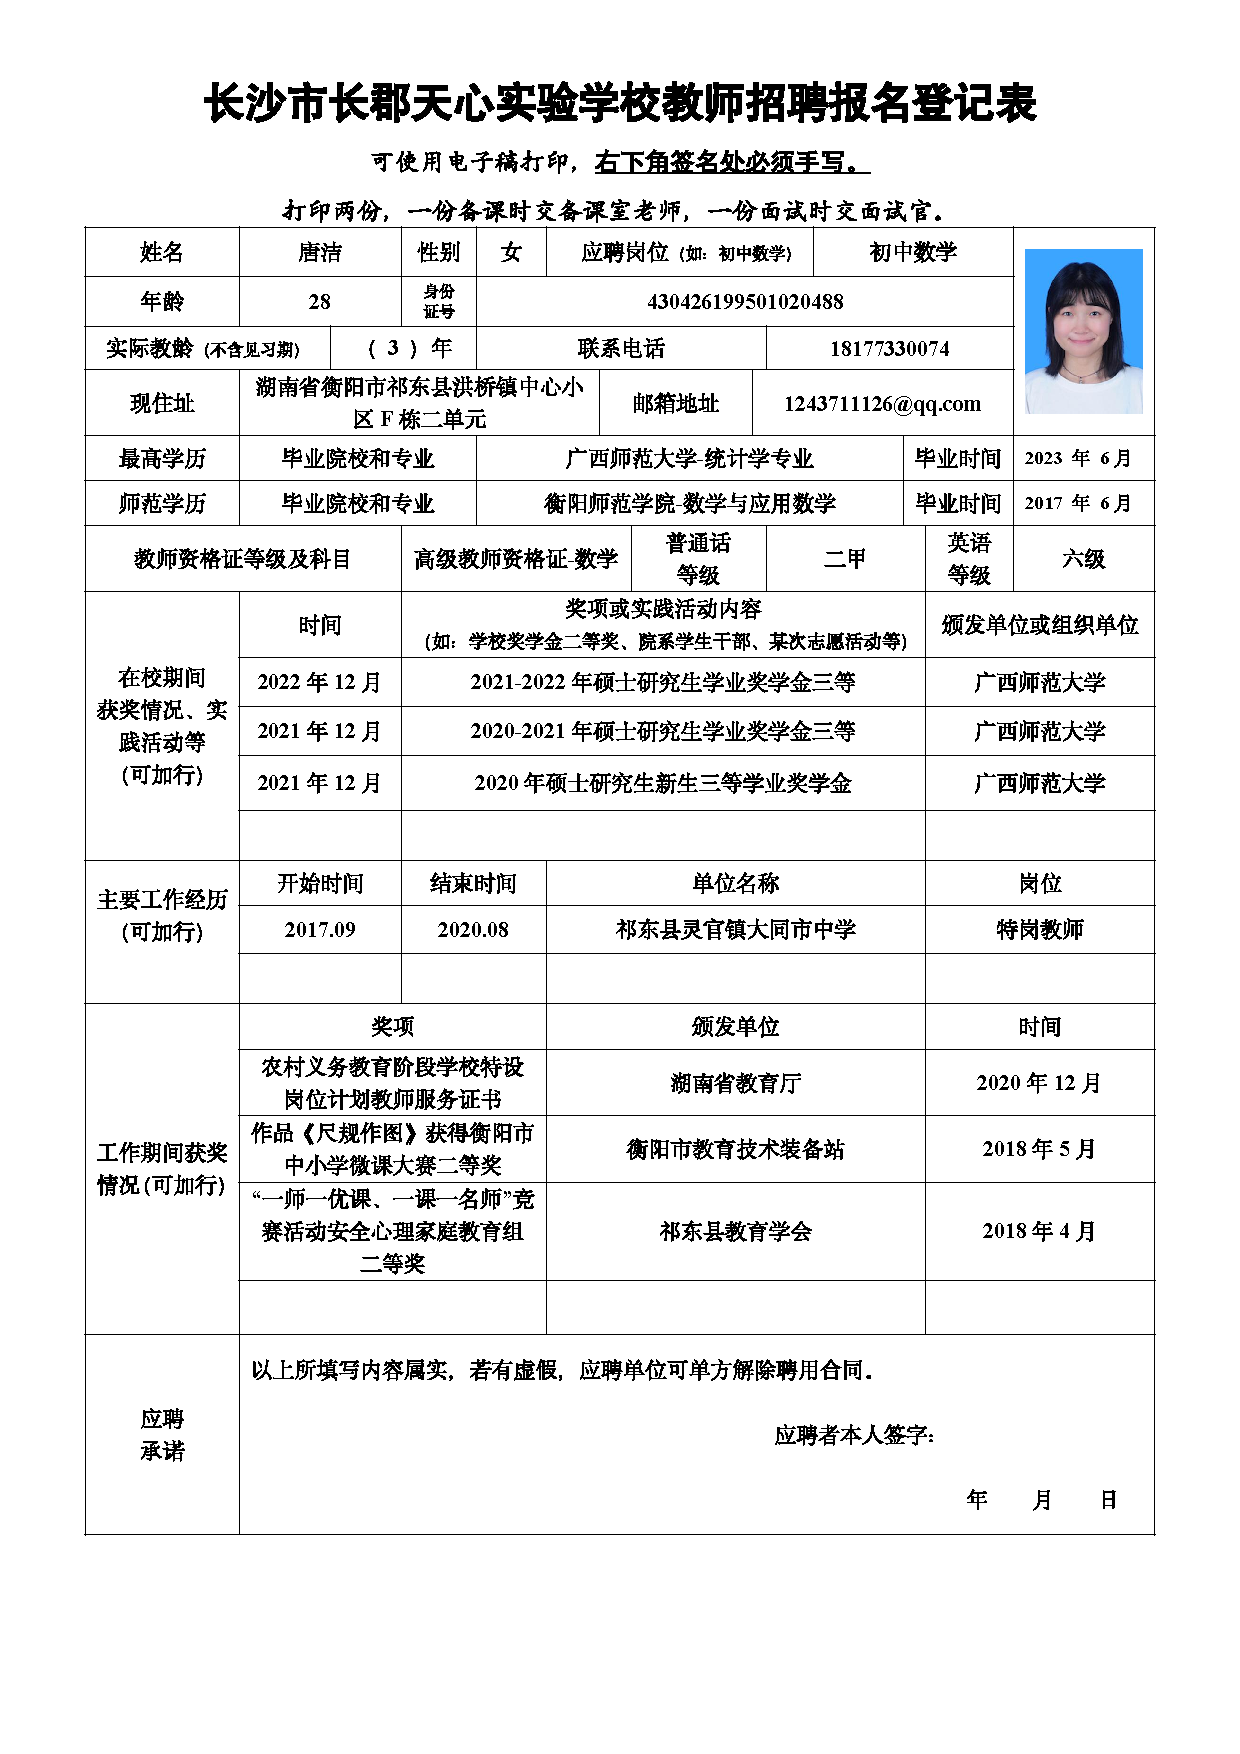
\includepdf[pages=1]{docs/6.29长沙市长郡天心实验学校教师招聘报名登记表.pdf}
%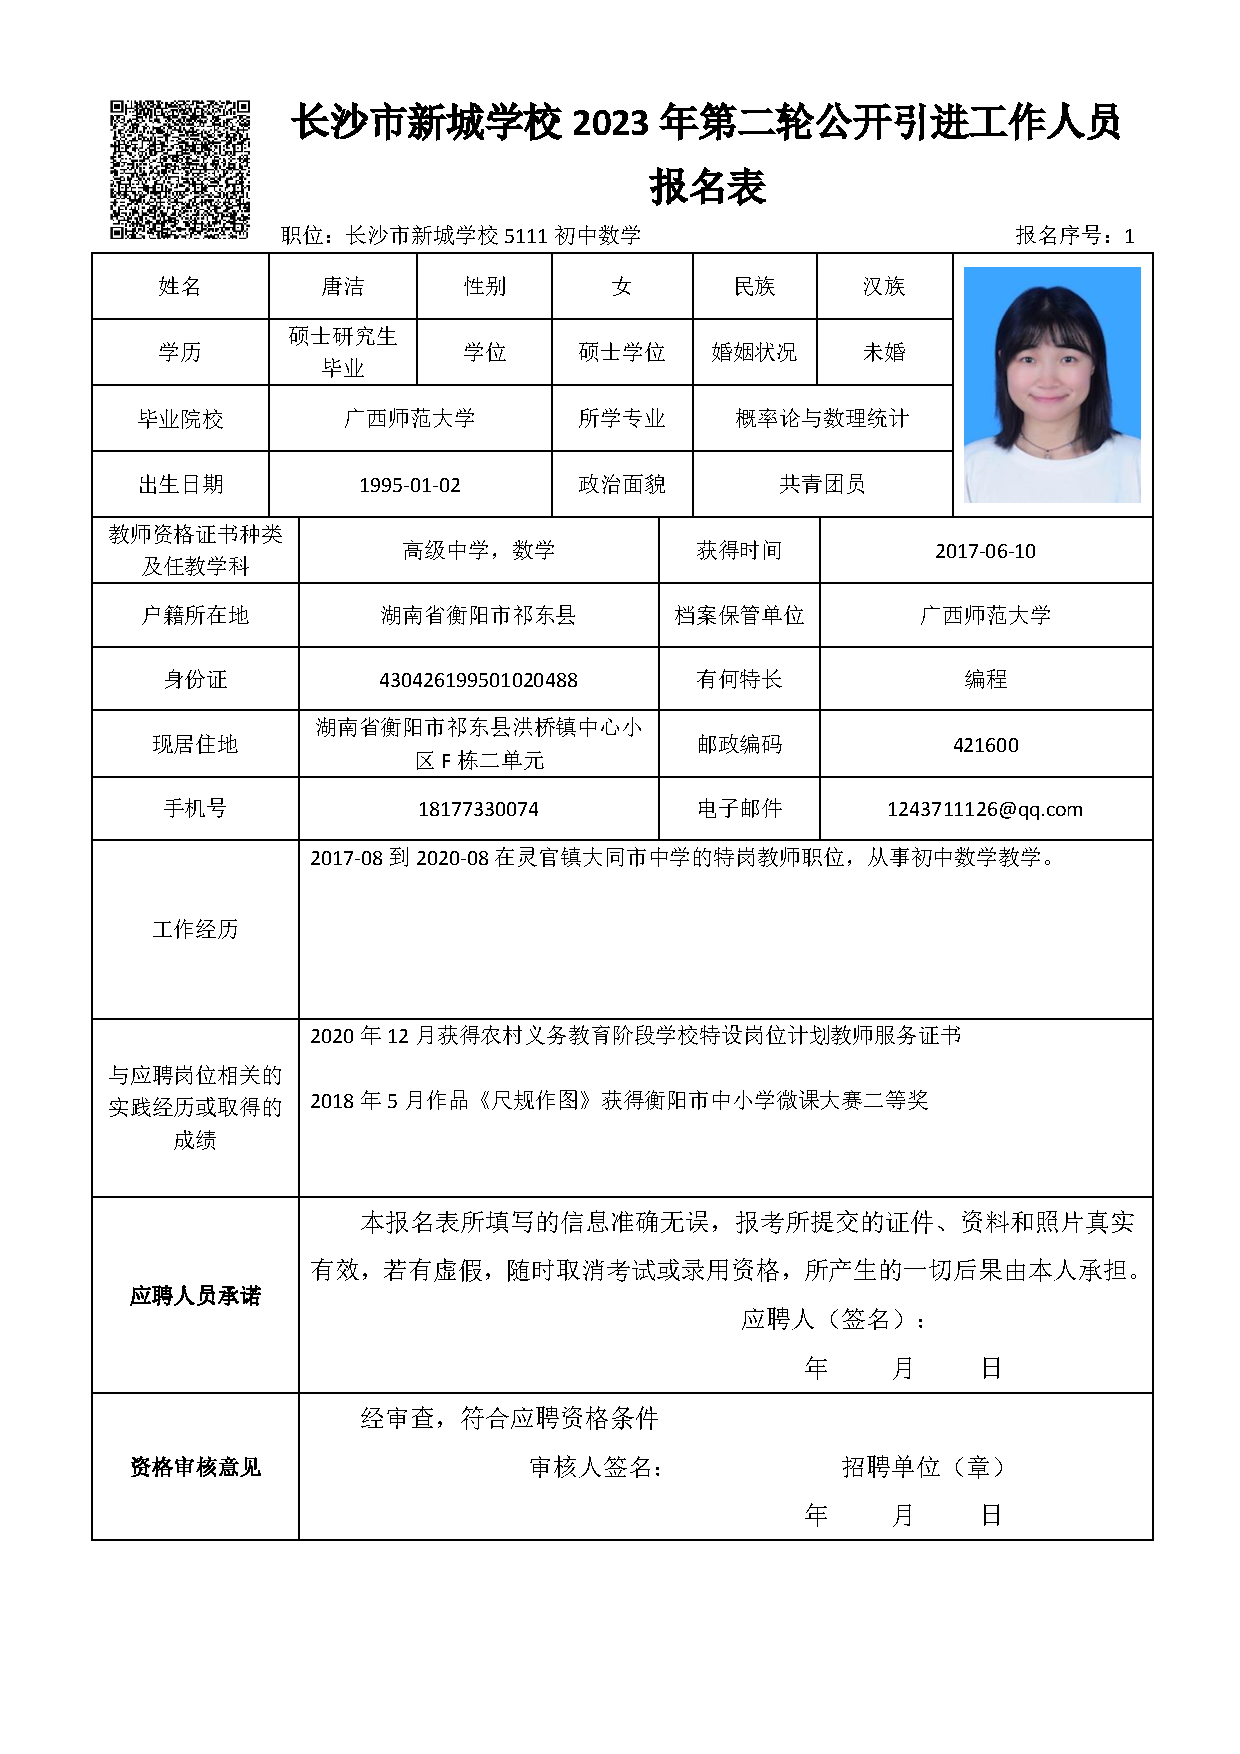
\includepdf[pages=1]{figs/二引/报名成功/5111长沙市新城学校报名表.pdf}
%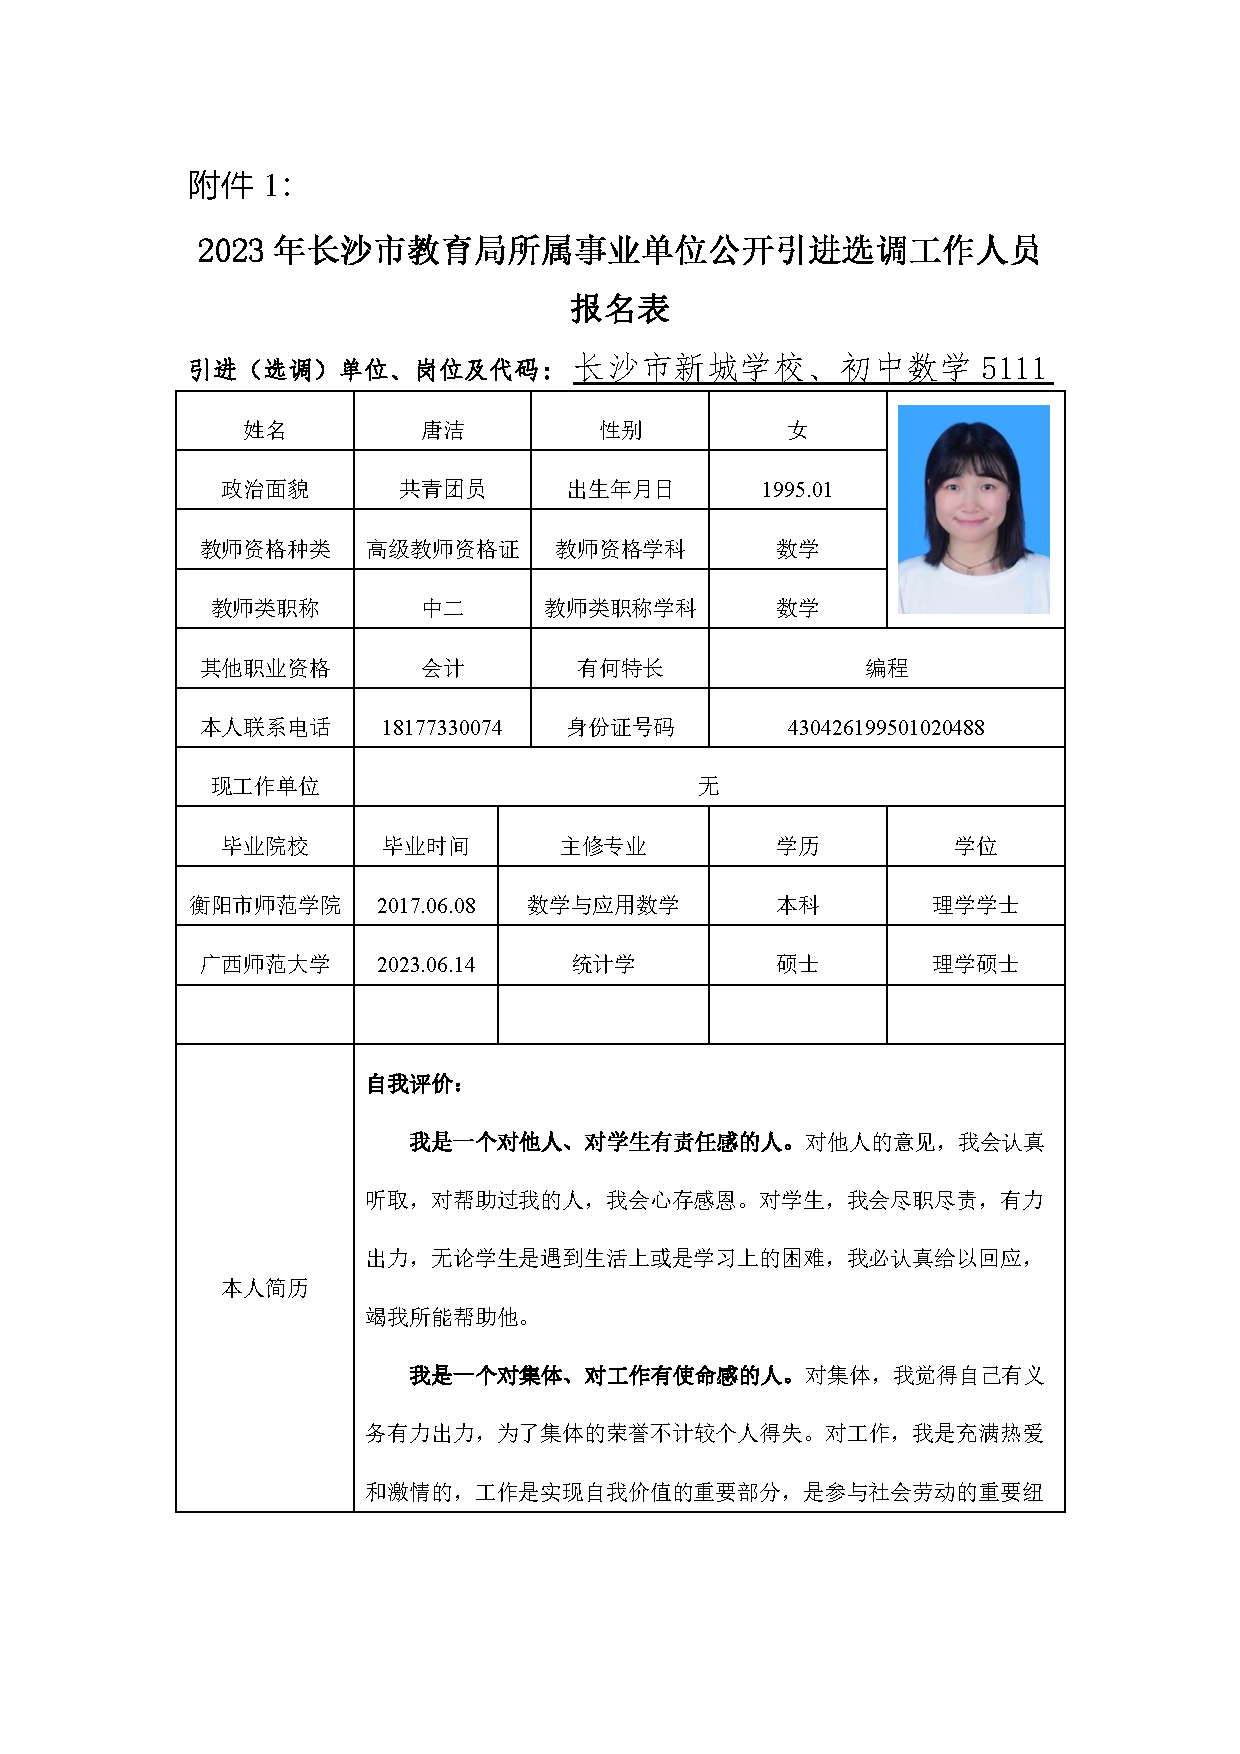
\includepdf[pages=1-2]{figs/二引/5111长沙市新城学校.pdf}
%
\includepdf[pages=1]{figs/二引/长沙二引承诺书.pdf}
%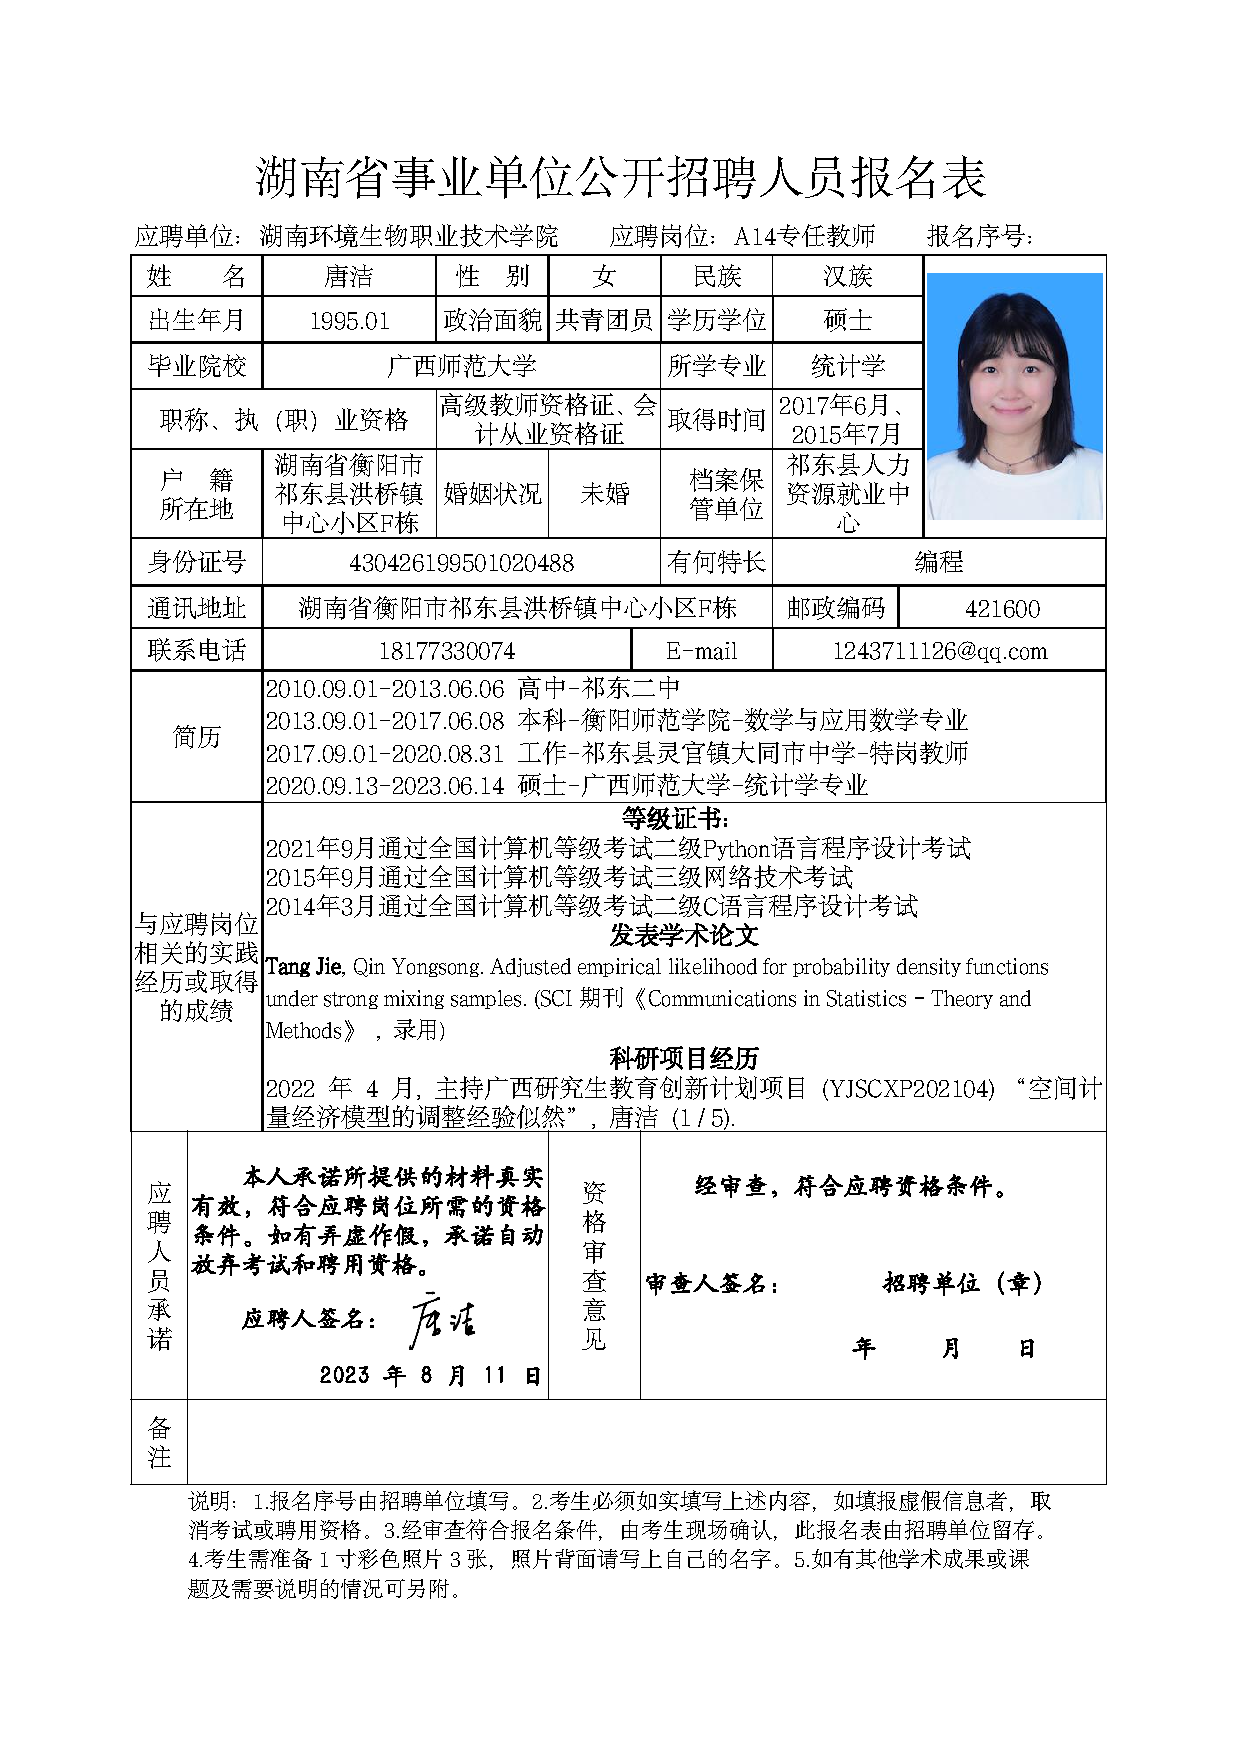
\includepdf[pages=1]{docs/湖南省事业单位公开招聘人员报名表.pdf}
%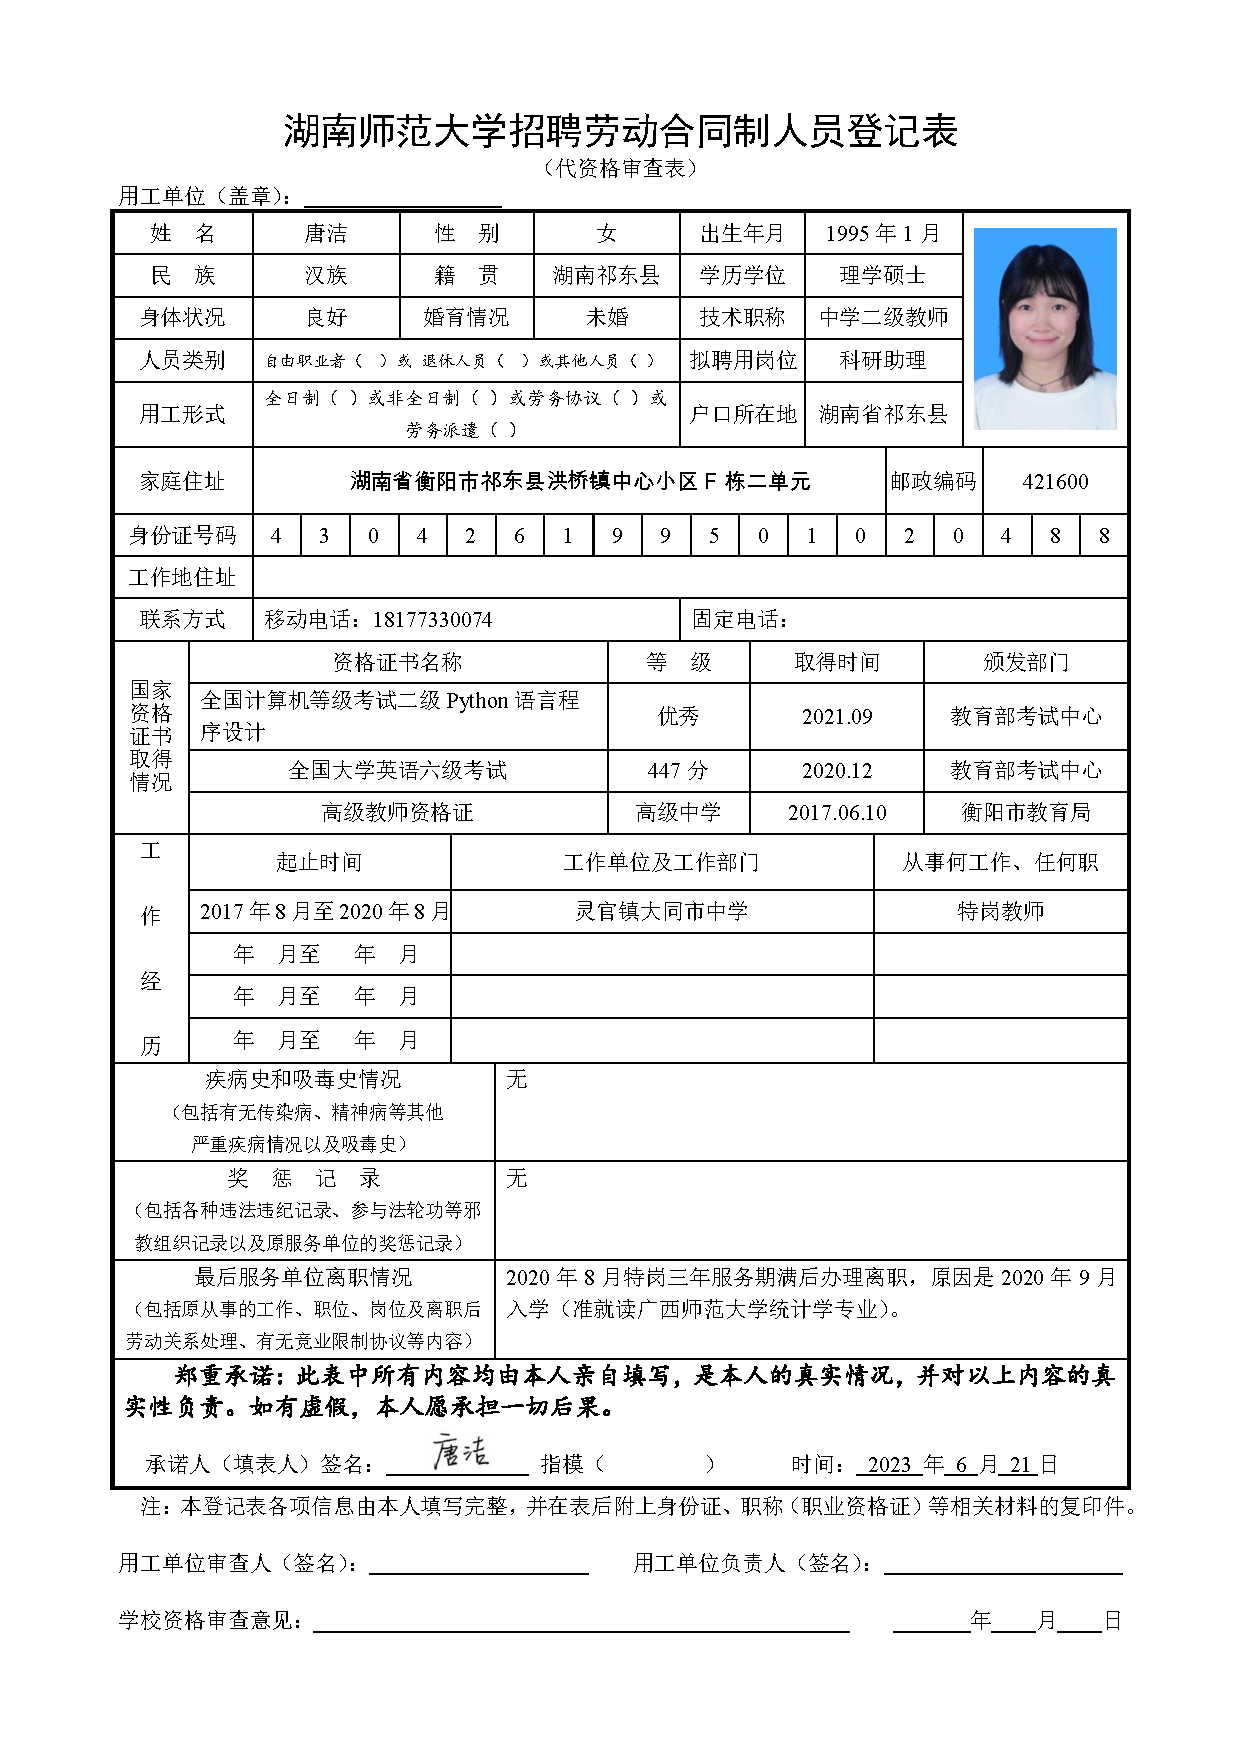
\includepdf[pages=1]{pdfs/湖南师范大学招聘劳动合同制人员登记表.pdf}
%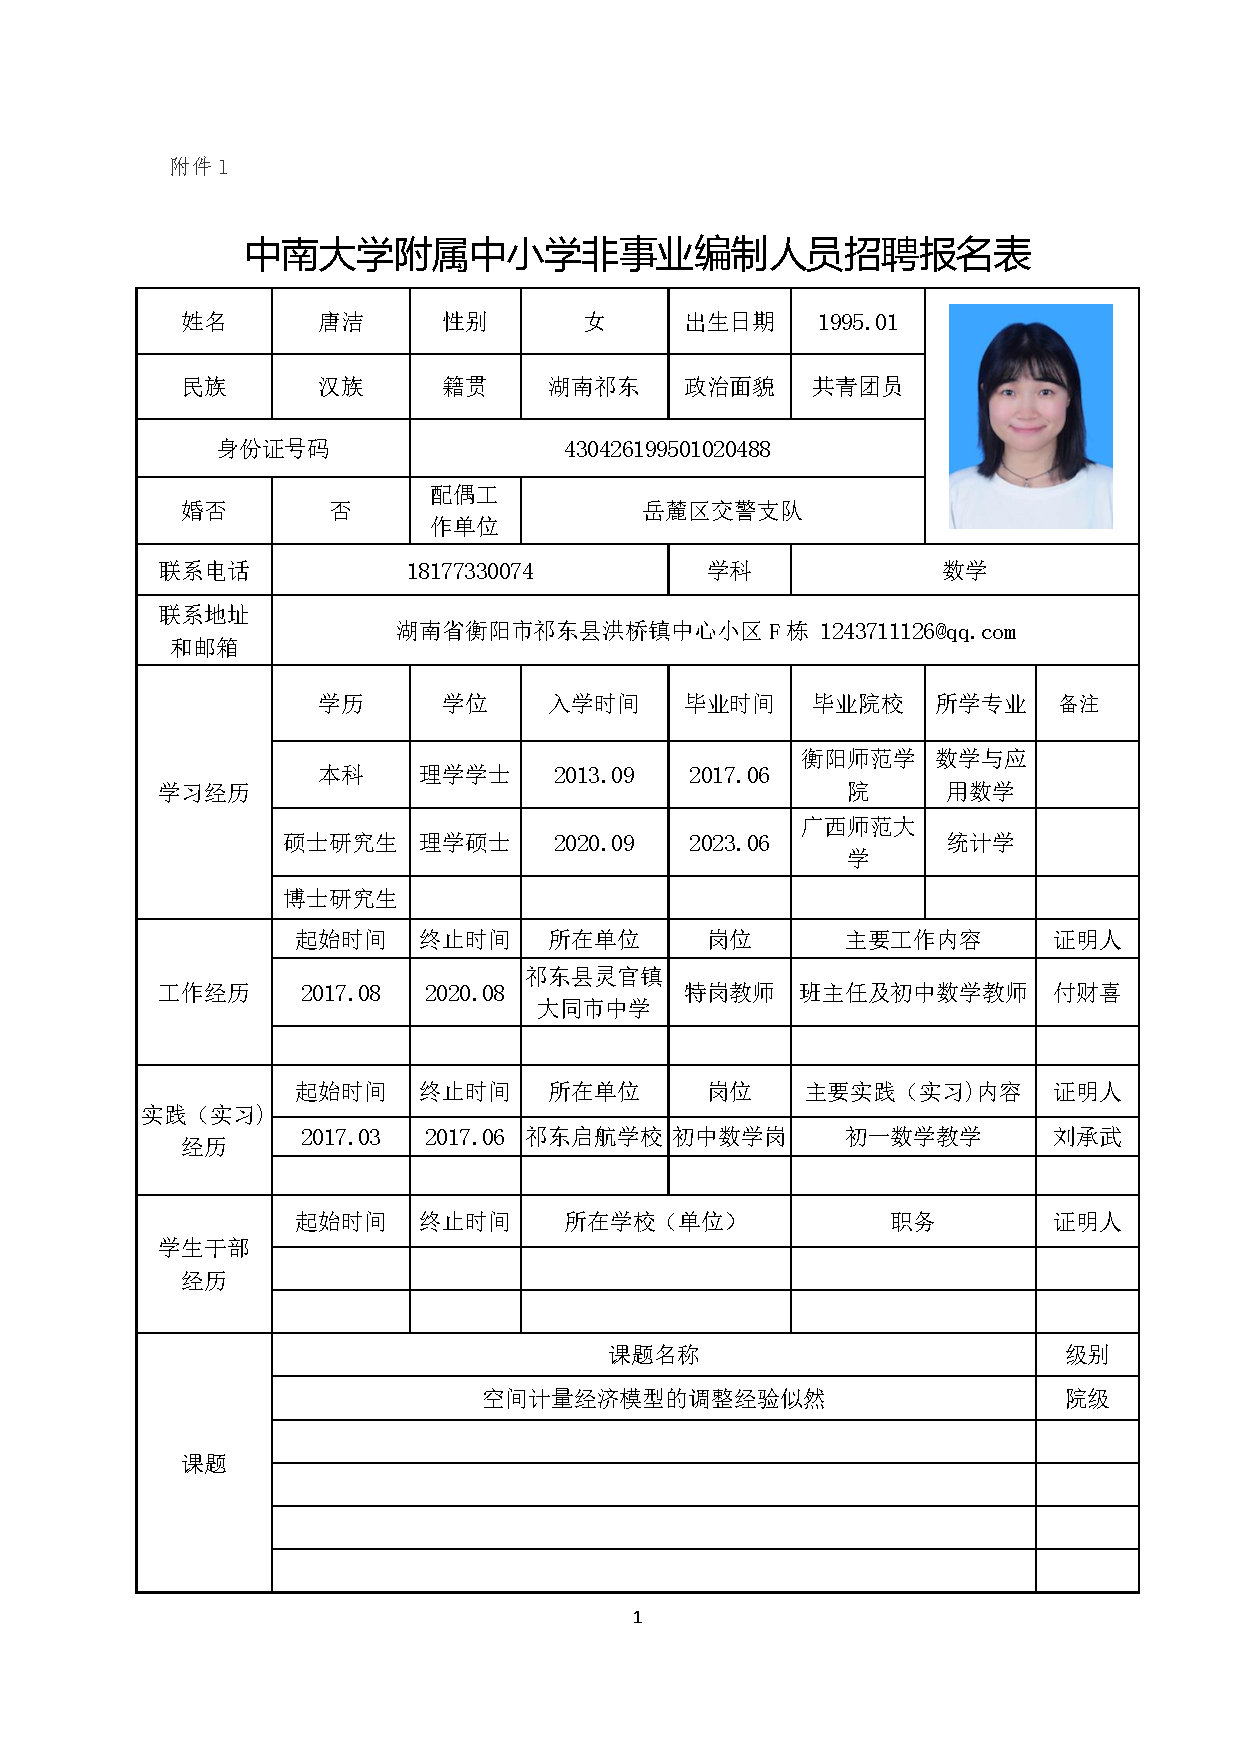
\includepdf[pages=1-2]{pdfs/中南大学附属中小学非事业编人员报名登记表.pdf}

\section{个人简历}
%%%
\includepdf[pages=2-3]{pdfs/简历2023-1.pdf}
%%%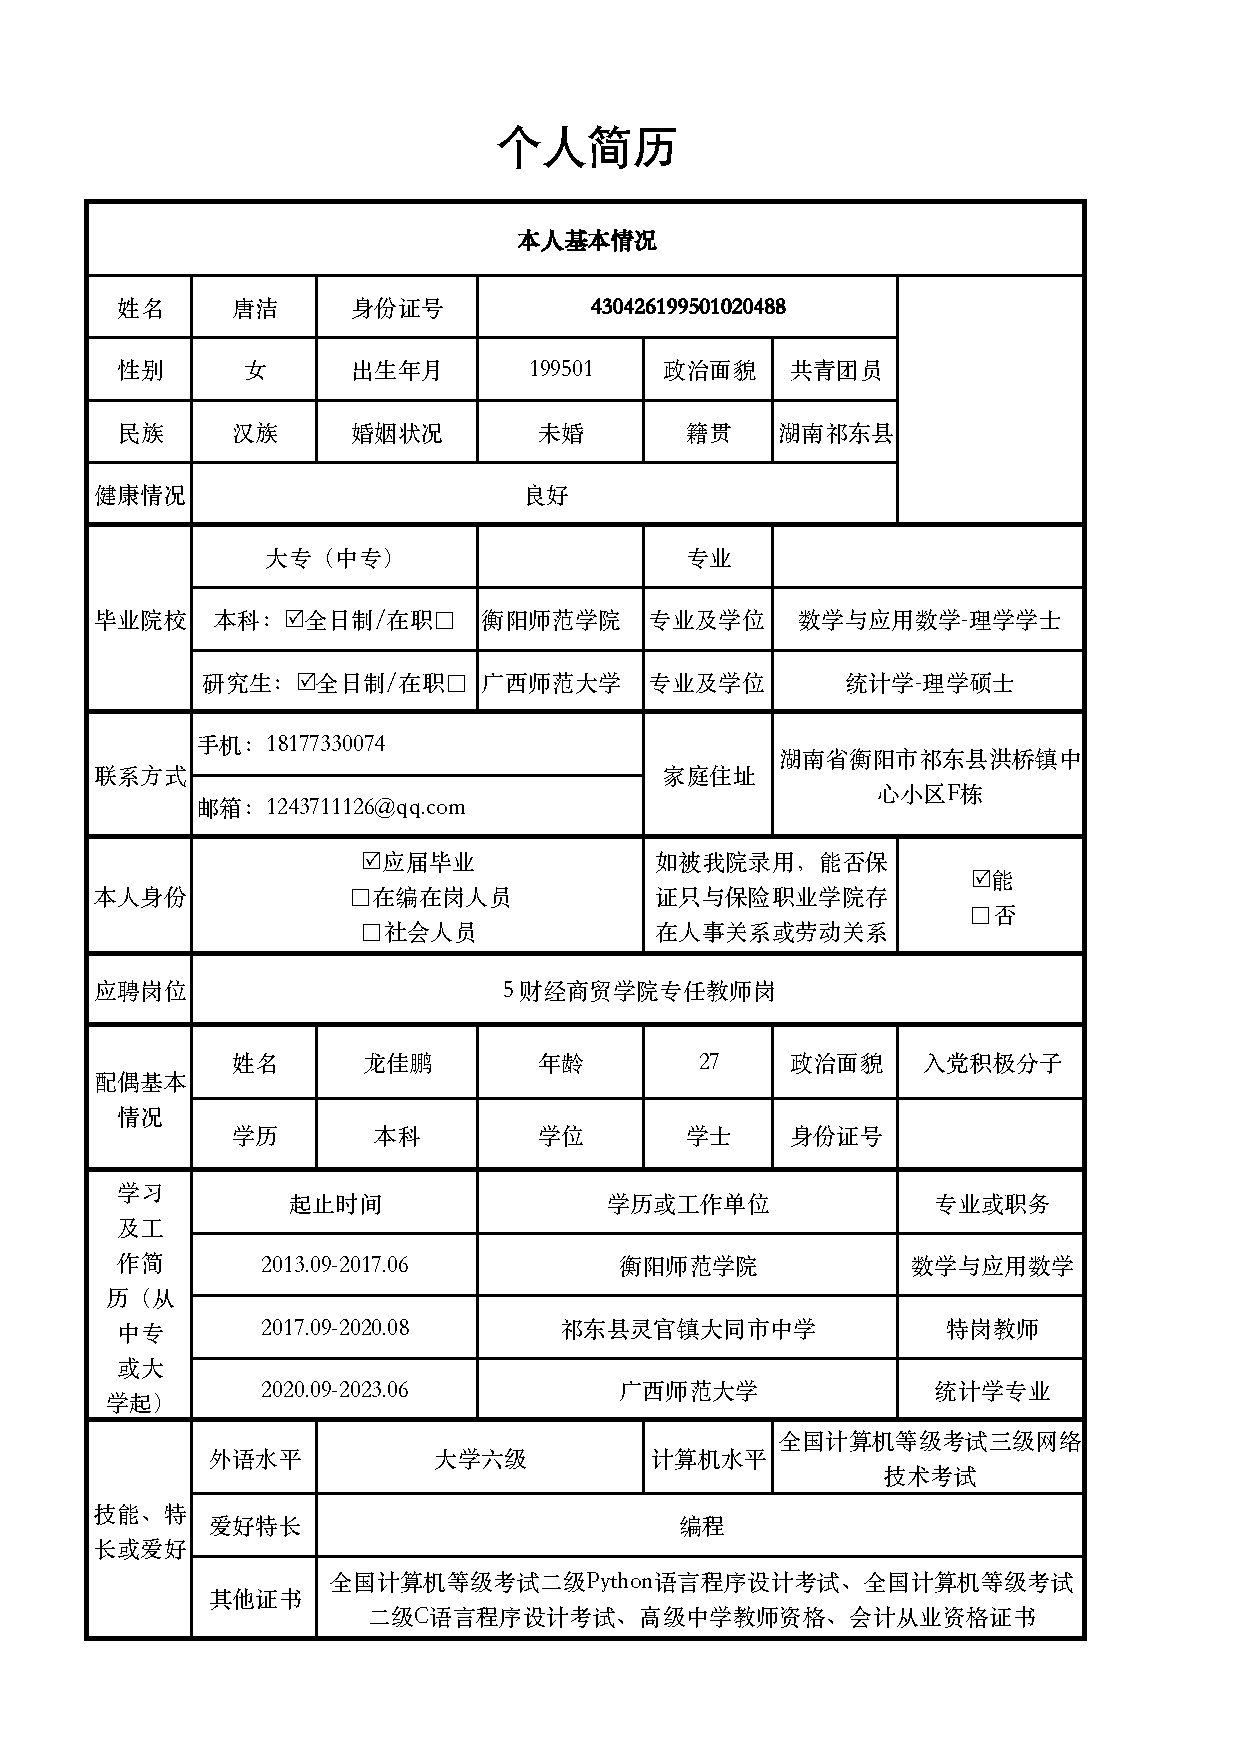
\includepdf[pages=1-2]{docs/保险职业学院招聘简历.pdf}
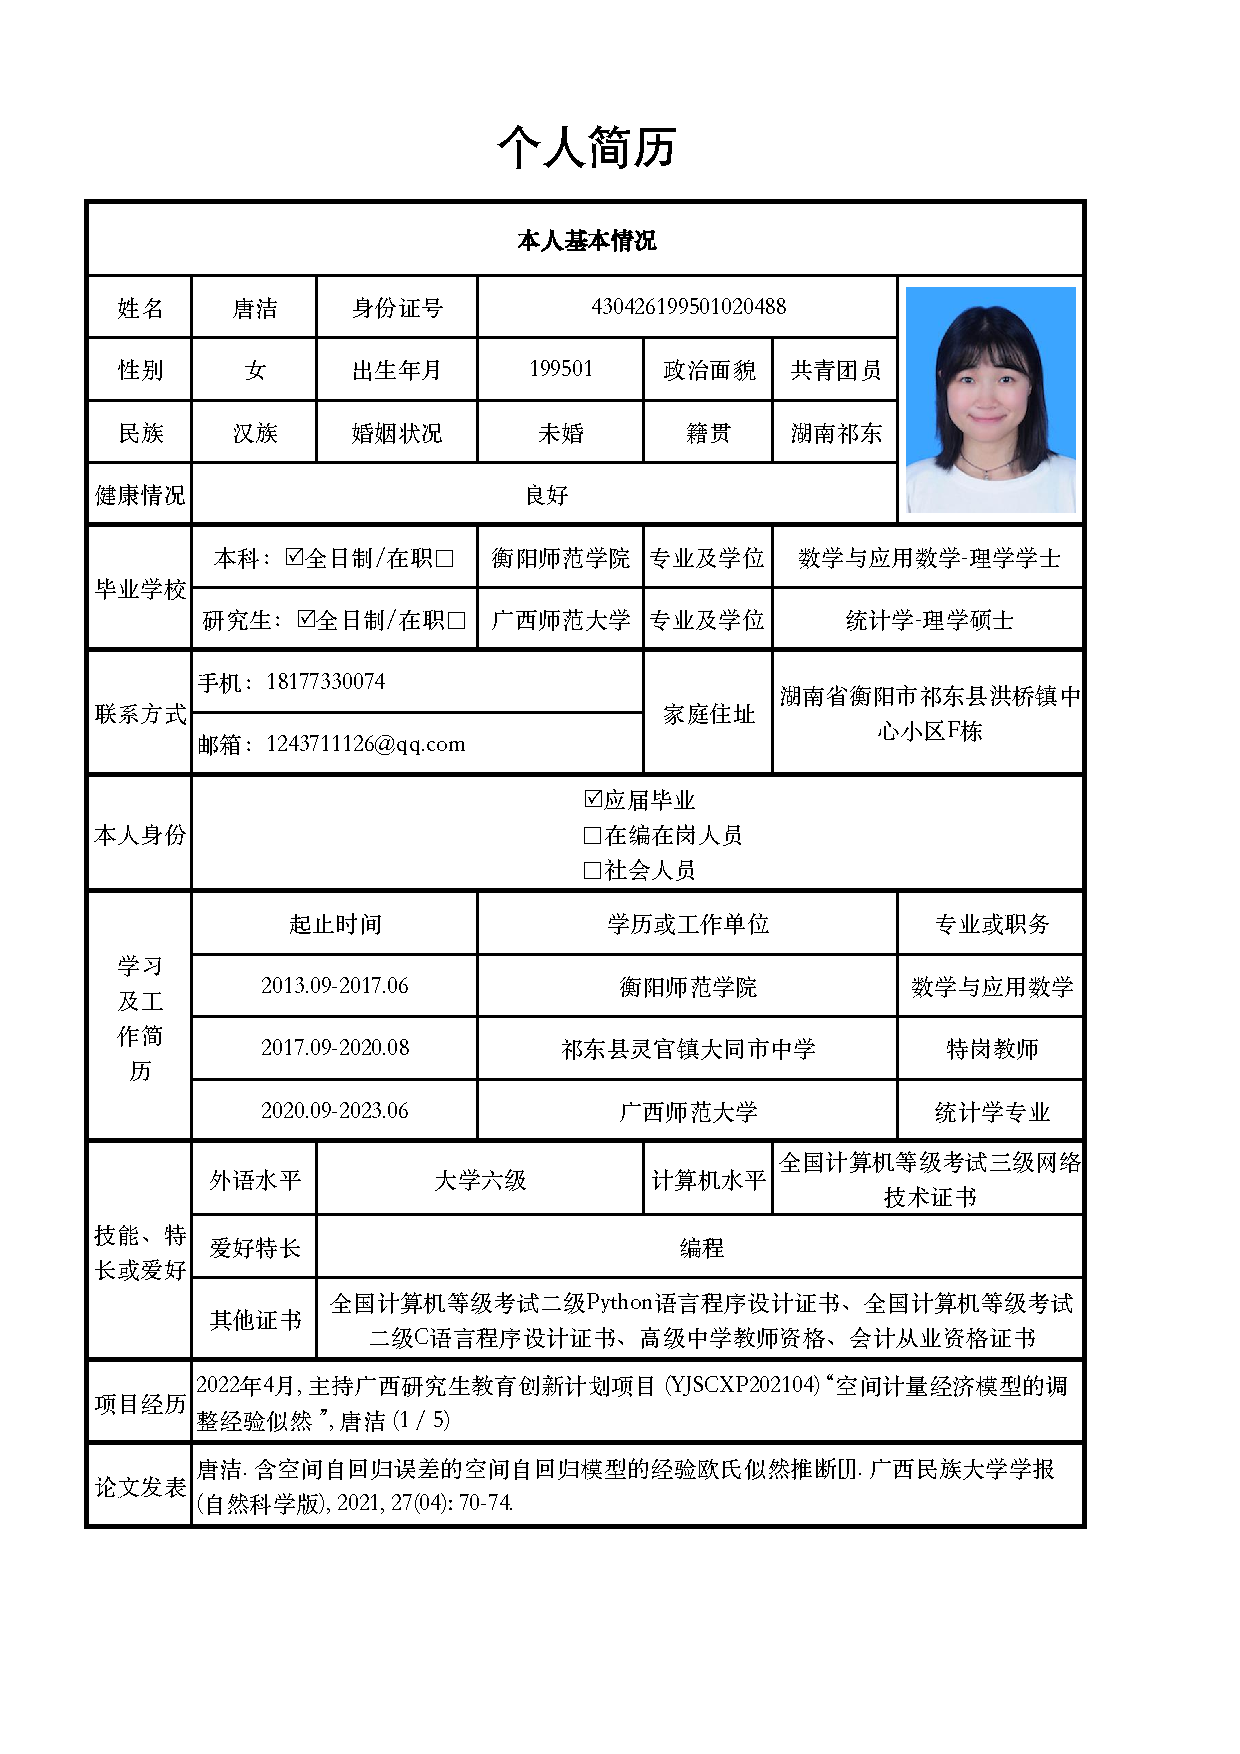
\includepdf[pages=1-2]{docs/唐洁简历excel1.pdf}

\section{相关材料}

\subsection{身份证}
\begin{center}
  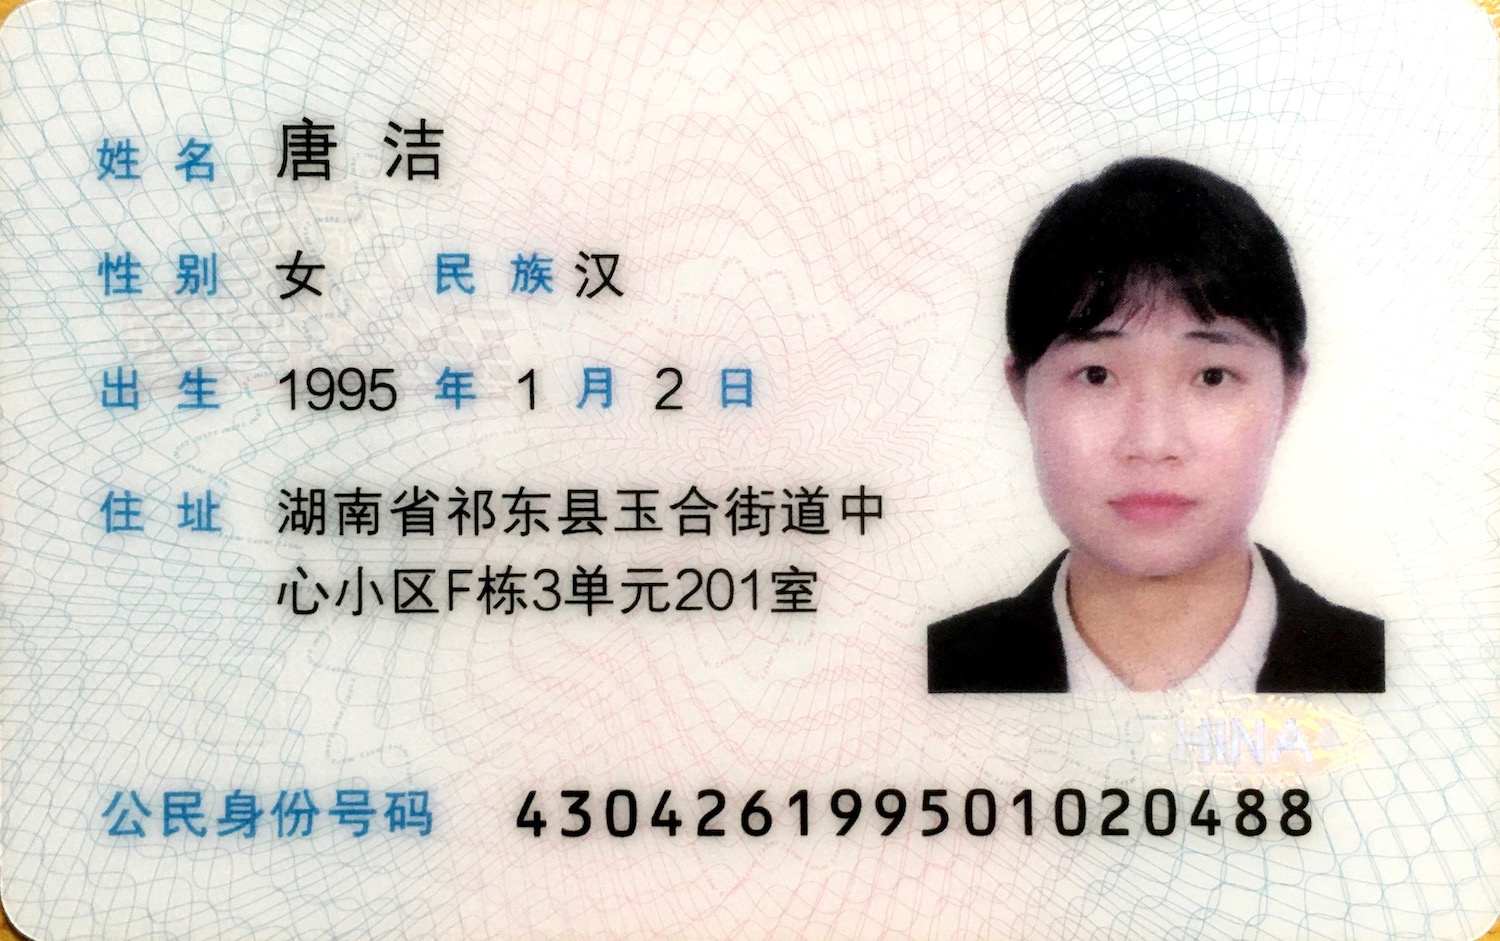
\includegraphics[scale=0.12]{figs/身份证1.jpg }
  
\includegraphics[scale=0.12]{figs/身份证2.jpg }
\end{center}

\subsection{学历证明}
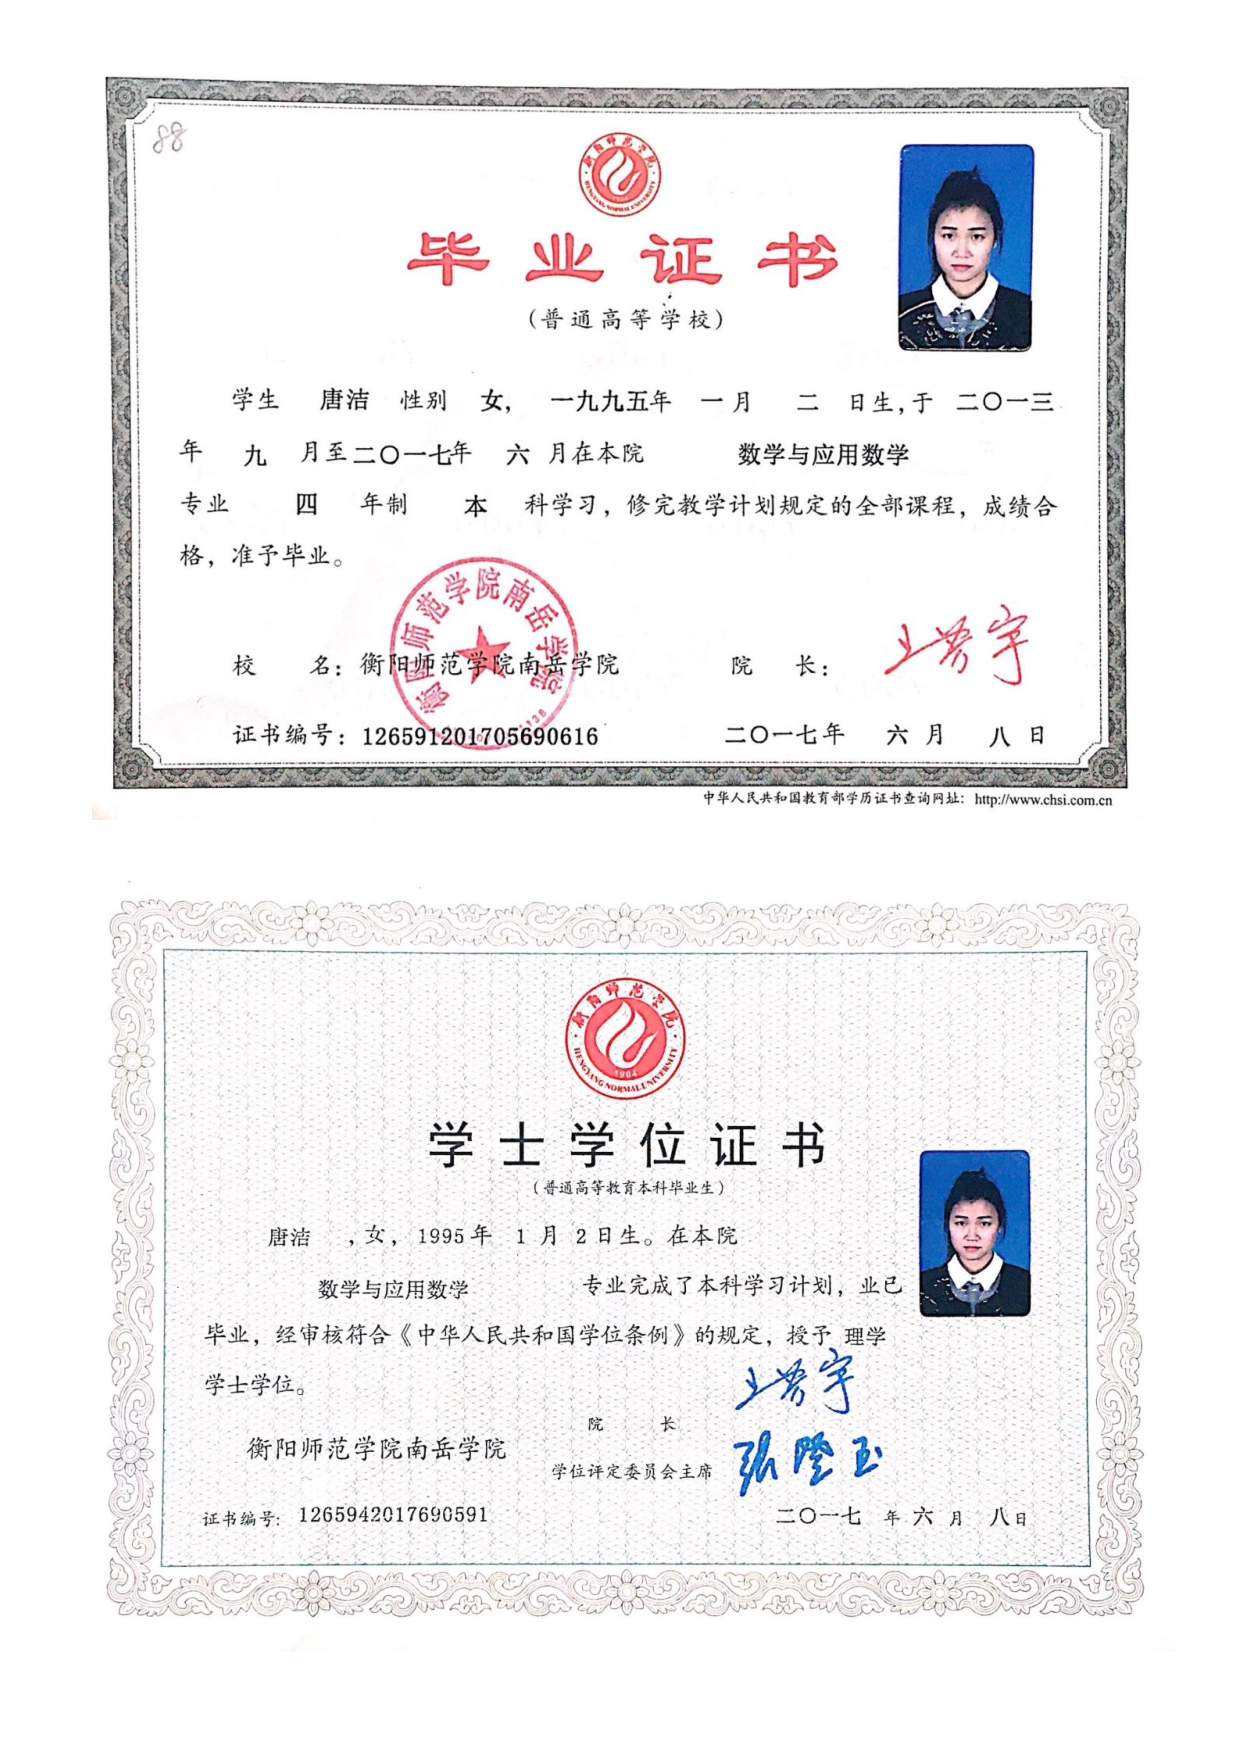
\includepdf[pages=1]{pdfs/毕业证与学位证本科.pdf}
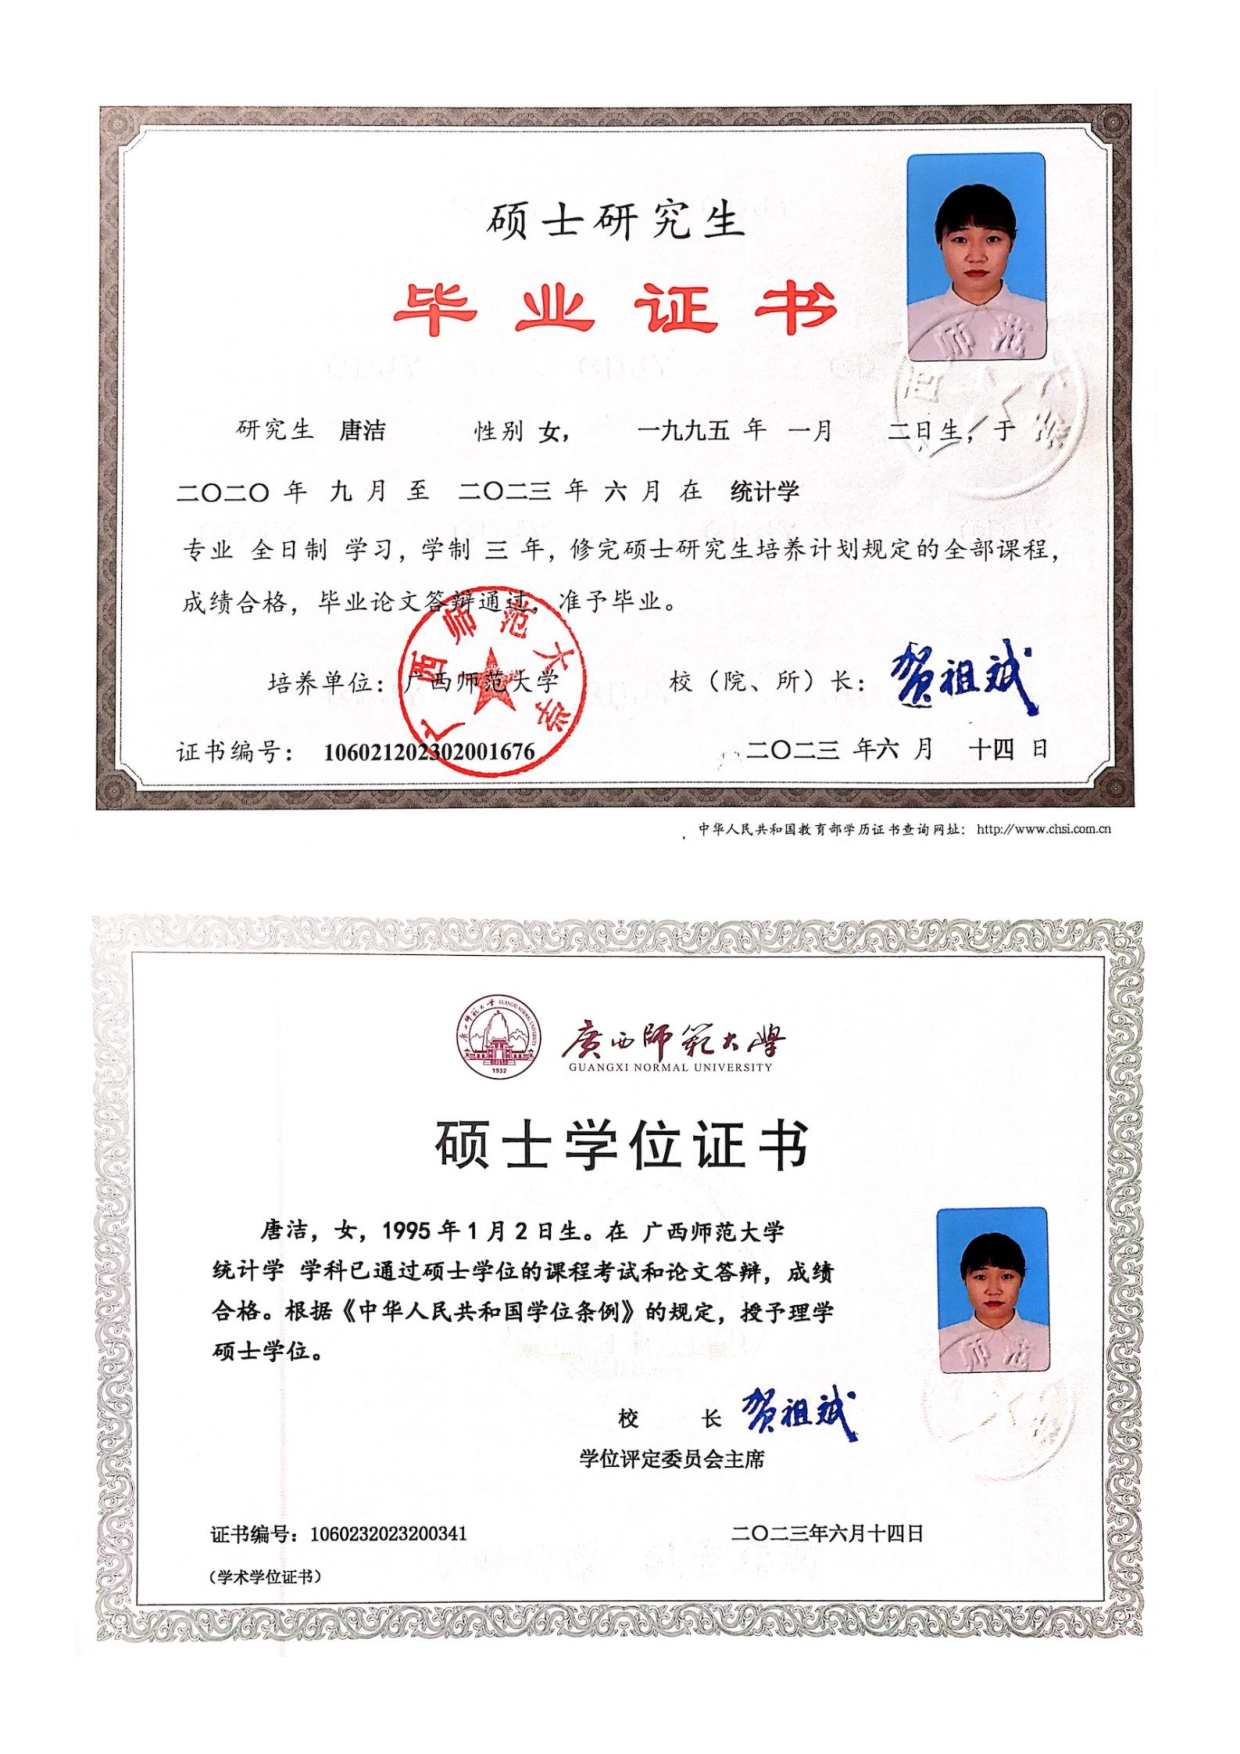
\includepdf[pages=1]{pdfs/毕业证与学位证硕士.pdf}
%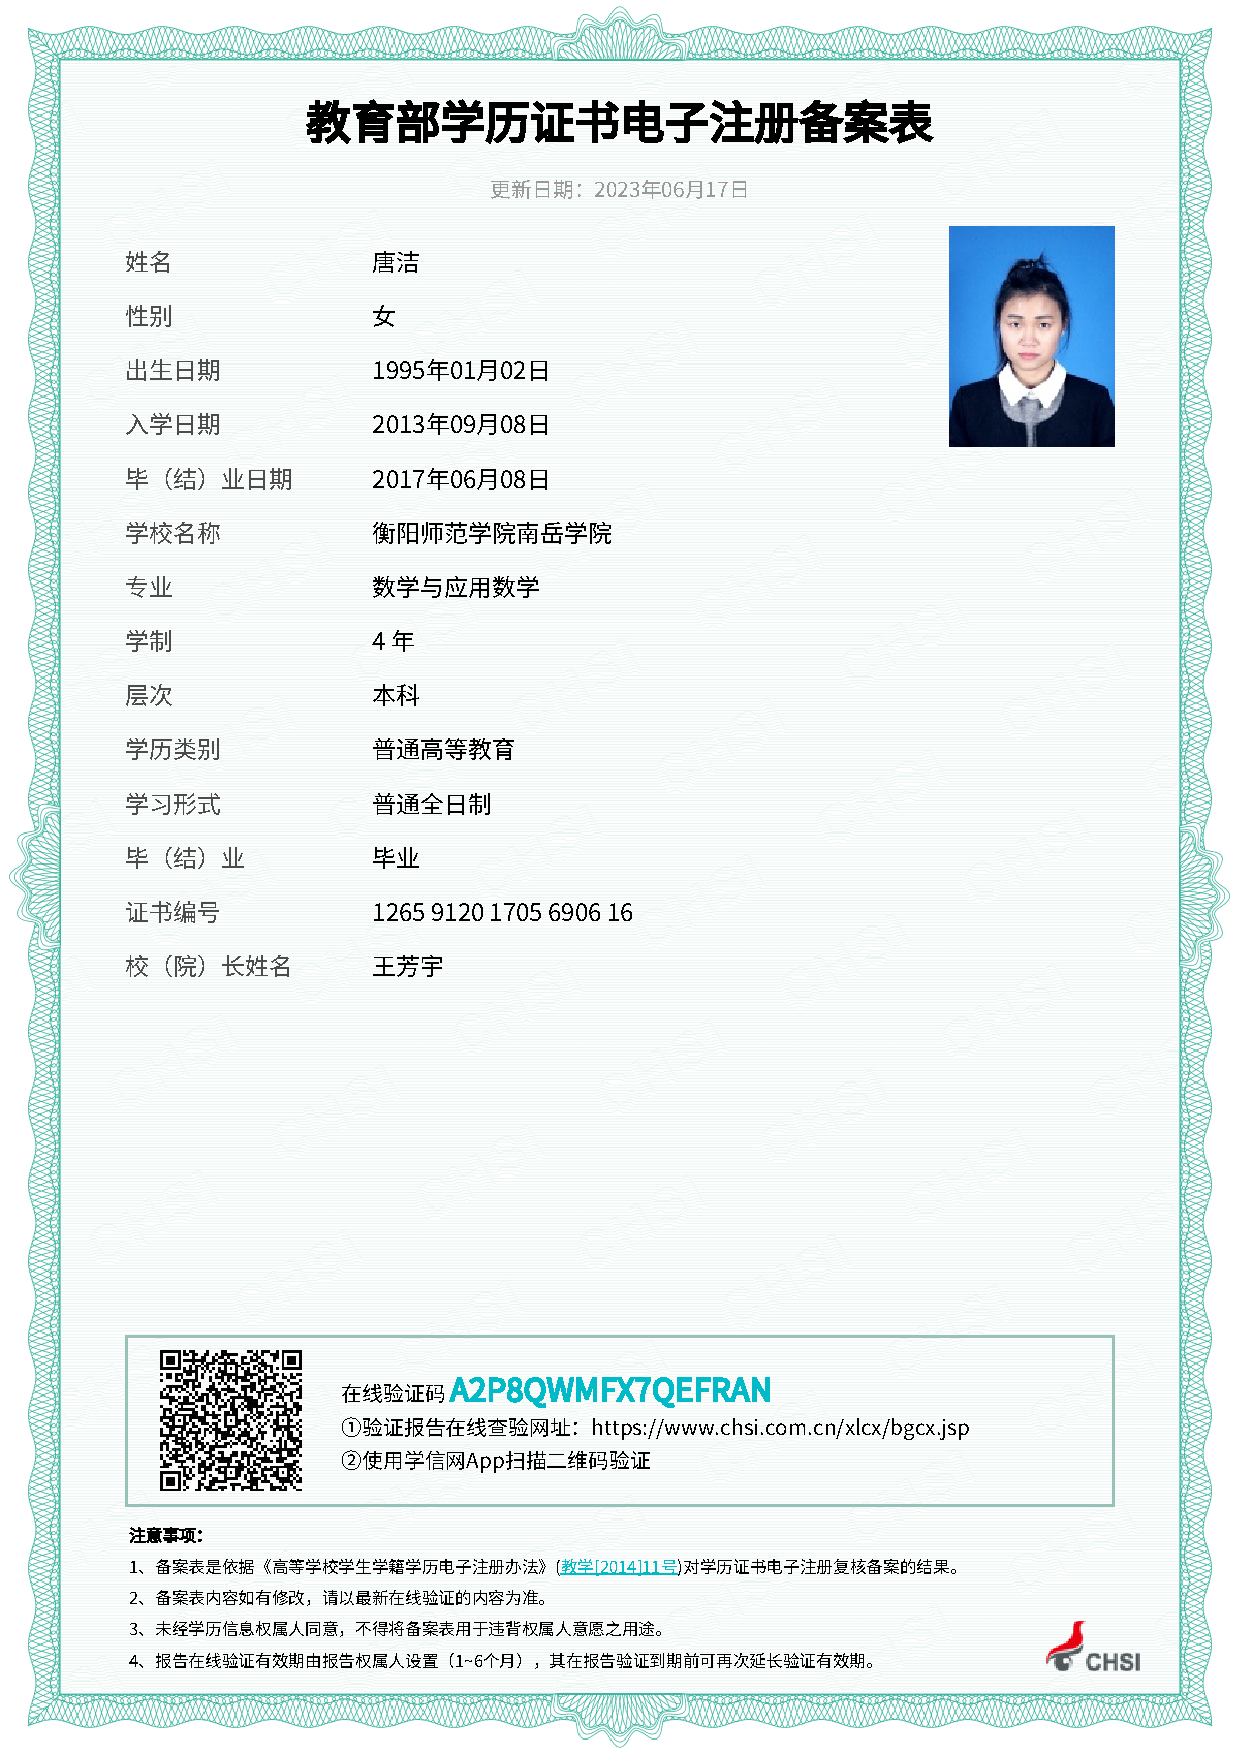
\includepdf[pages=1]{pdfs/教育部学历证书电子注册备案表本科.pdf}
%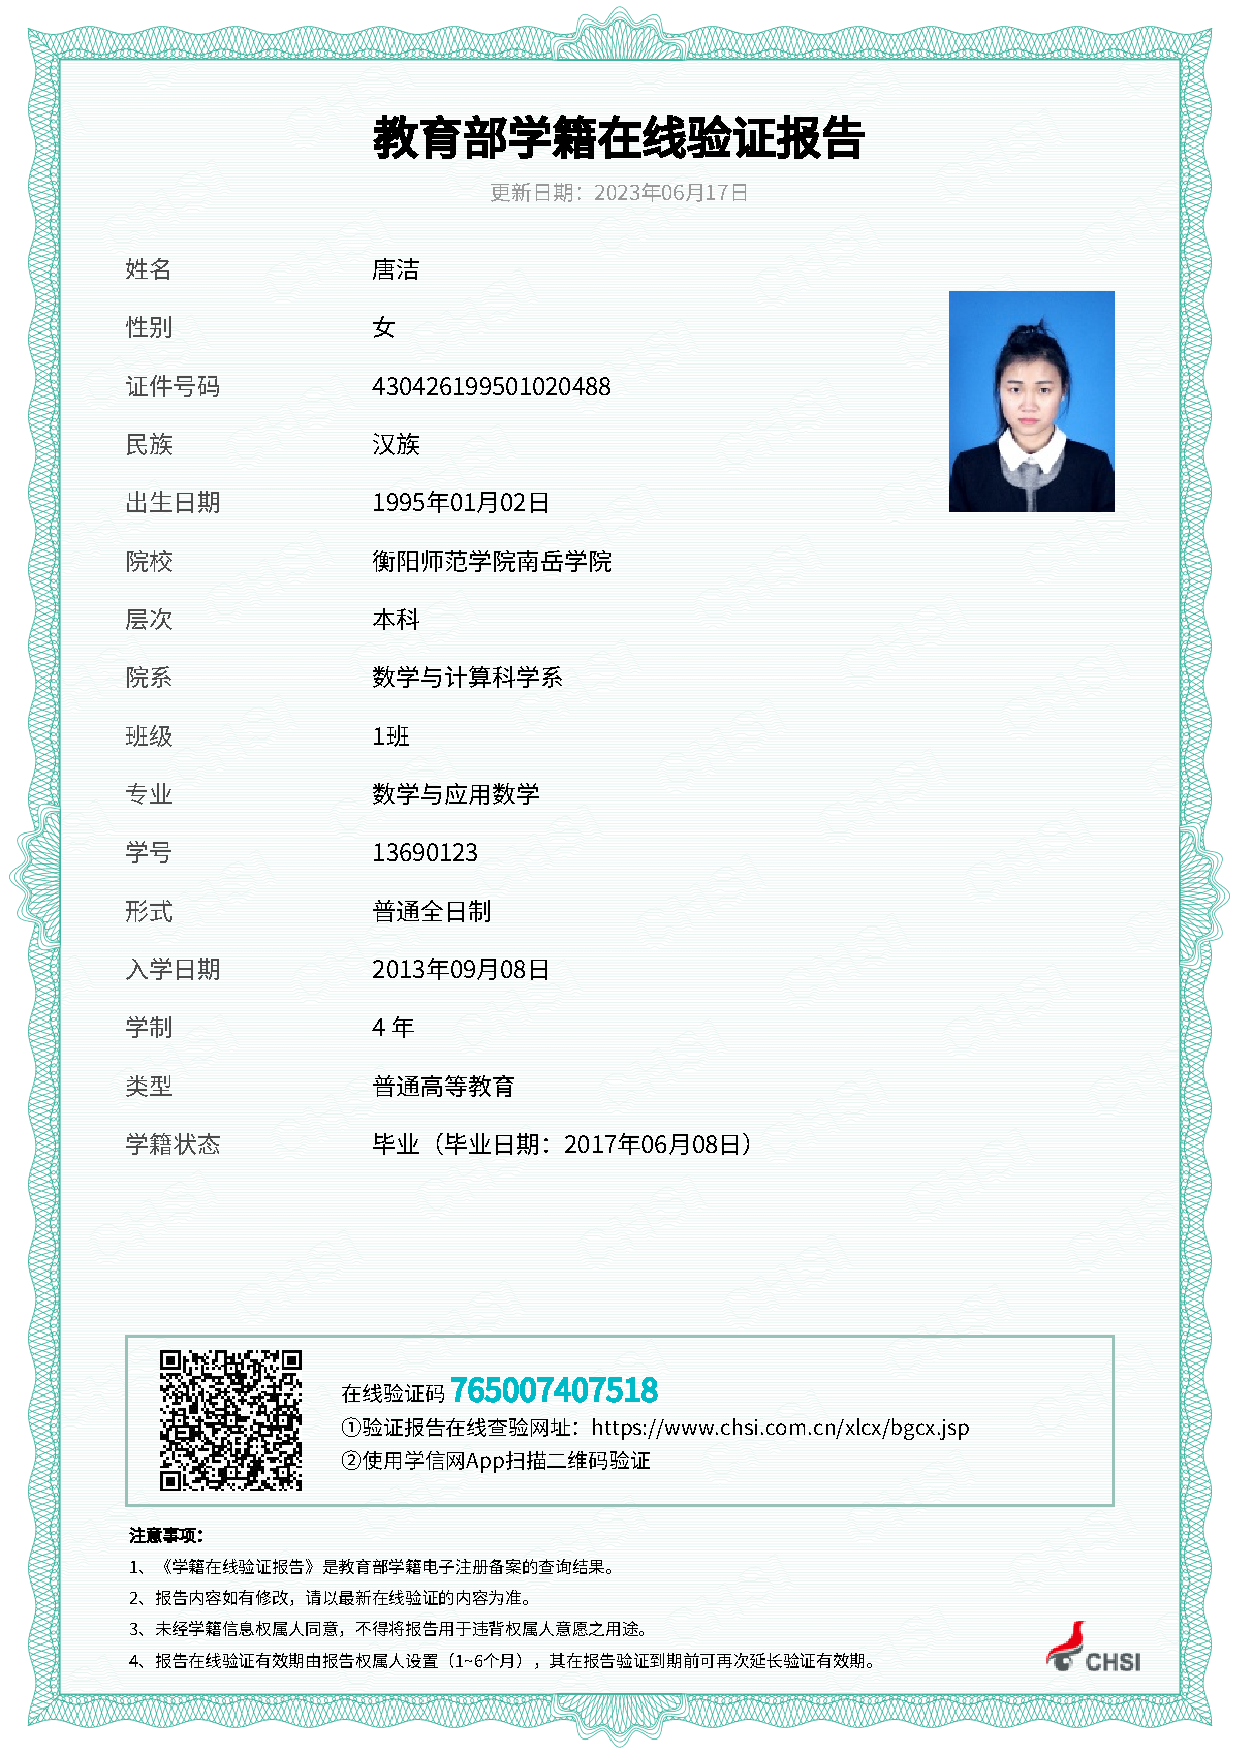
\includepdf[pages=1]{pdfs/教育部学籍在线验证报告本科.pdf}
%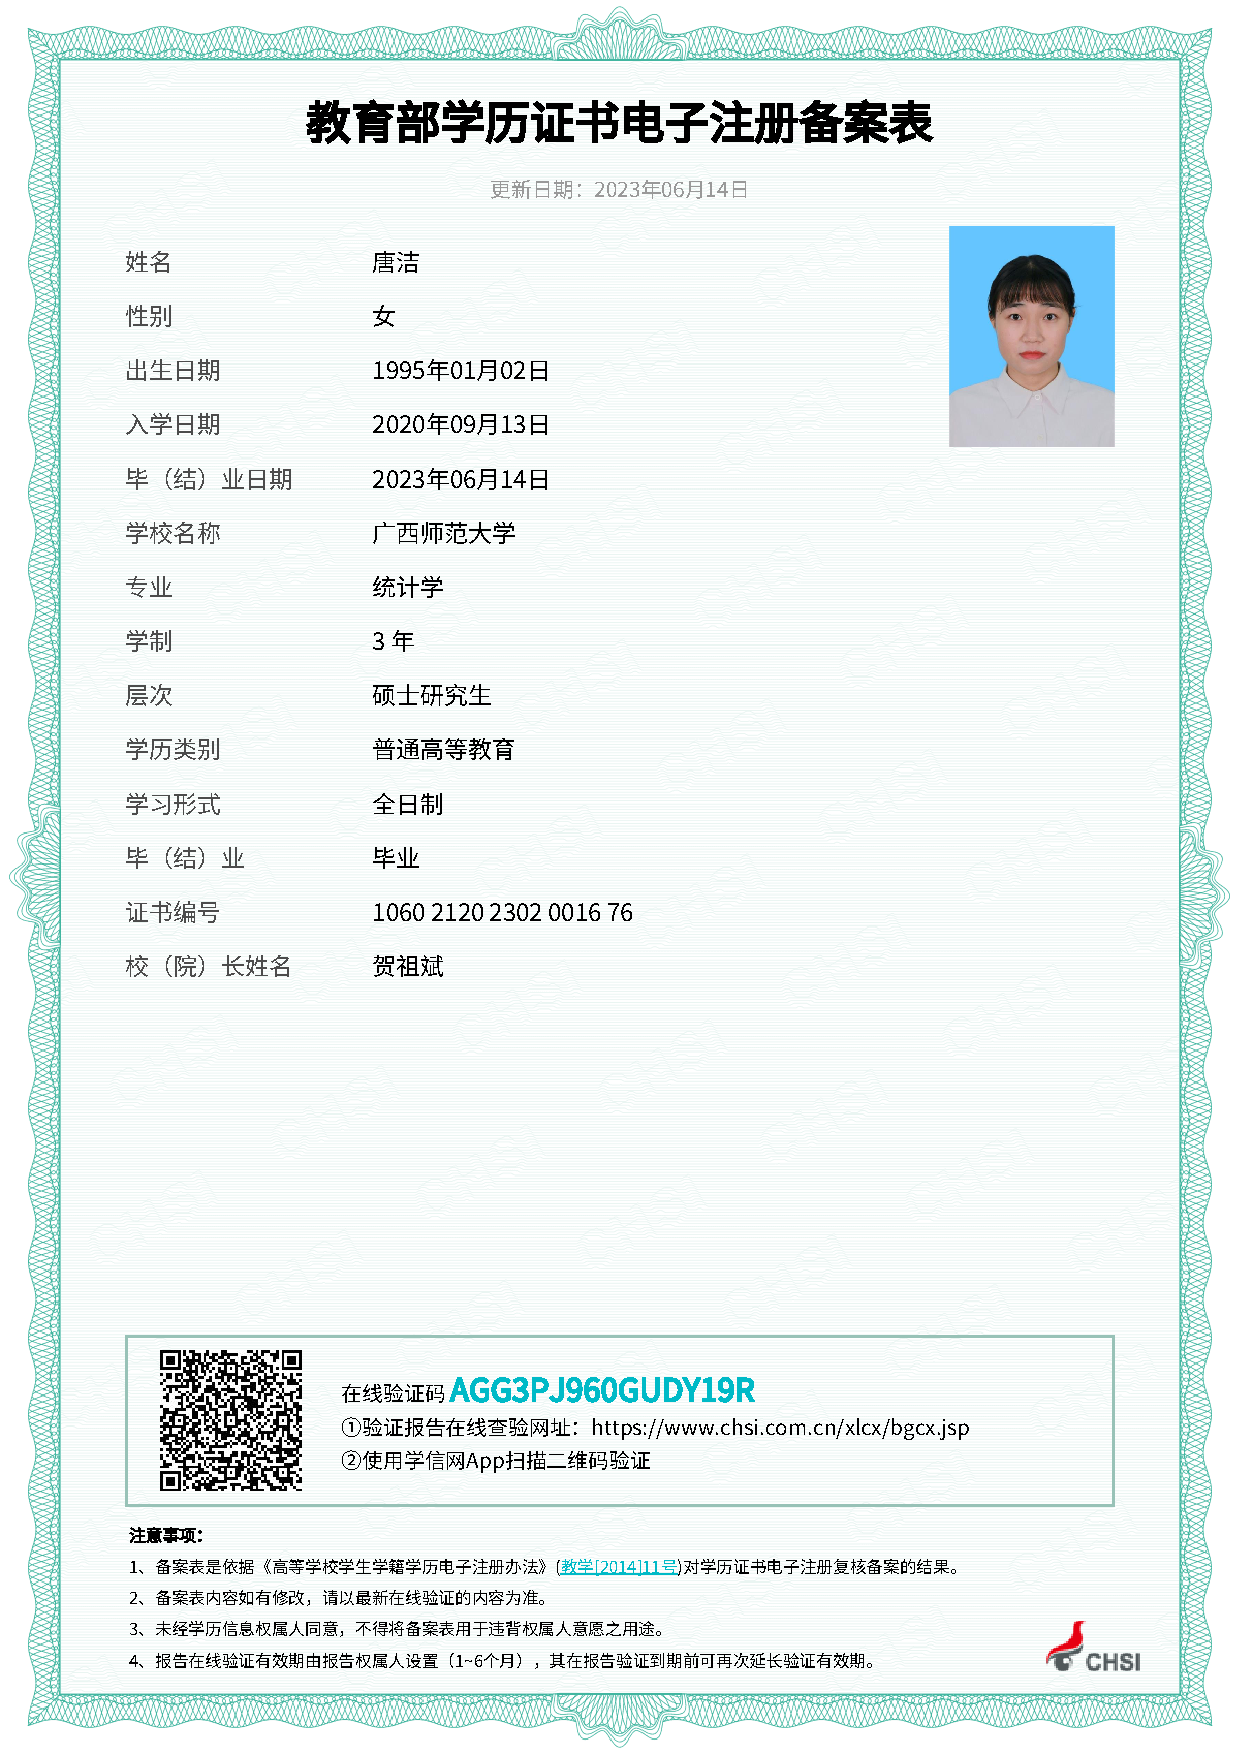
\includepdf[pages=1]{pdfs/教育部学历证书电子注册备案表硕士.pdf}
%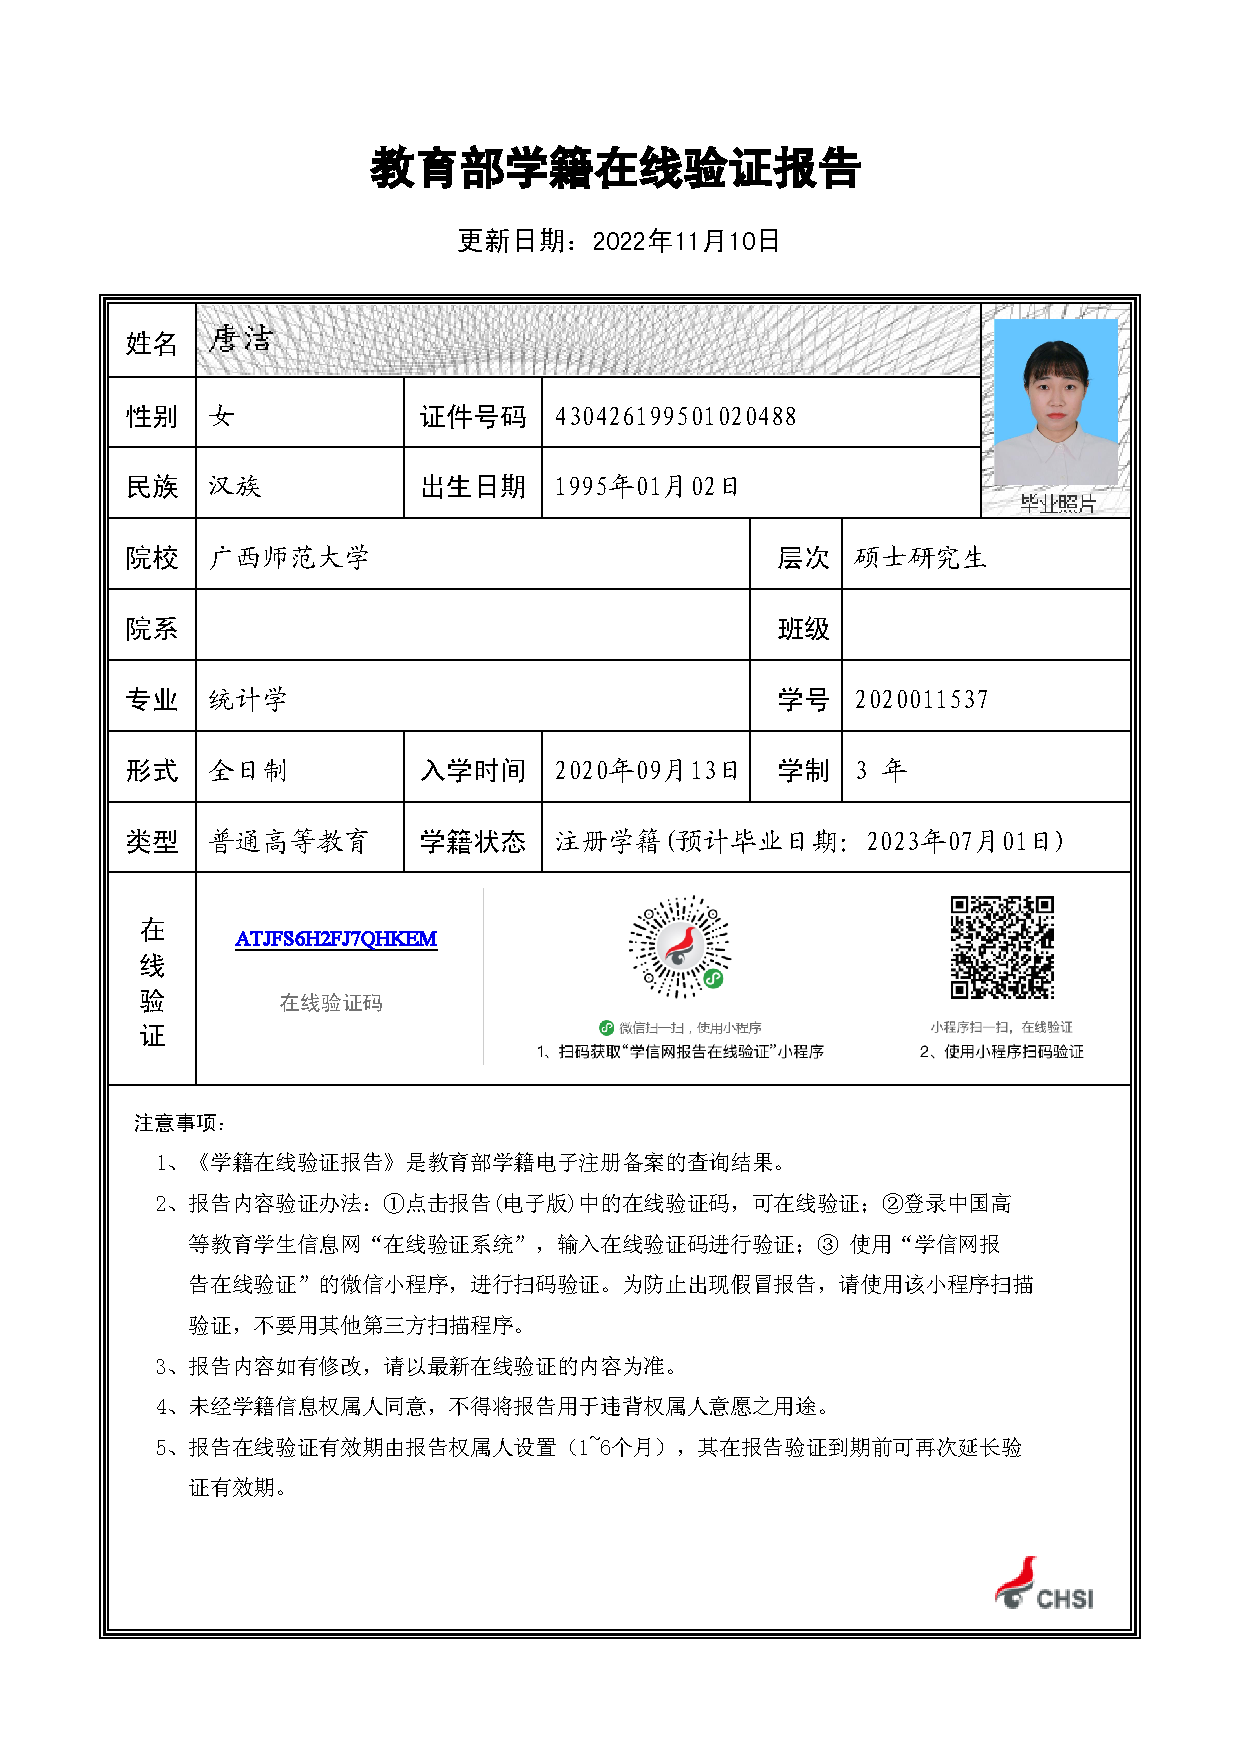
\includepdf[pages=1]{pdfs/教育部学籍在线验证报告硕士.pdf}

%\subsection{就业推荐表}
%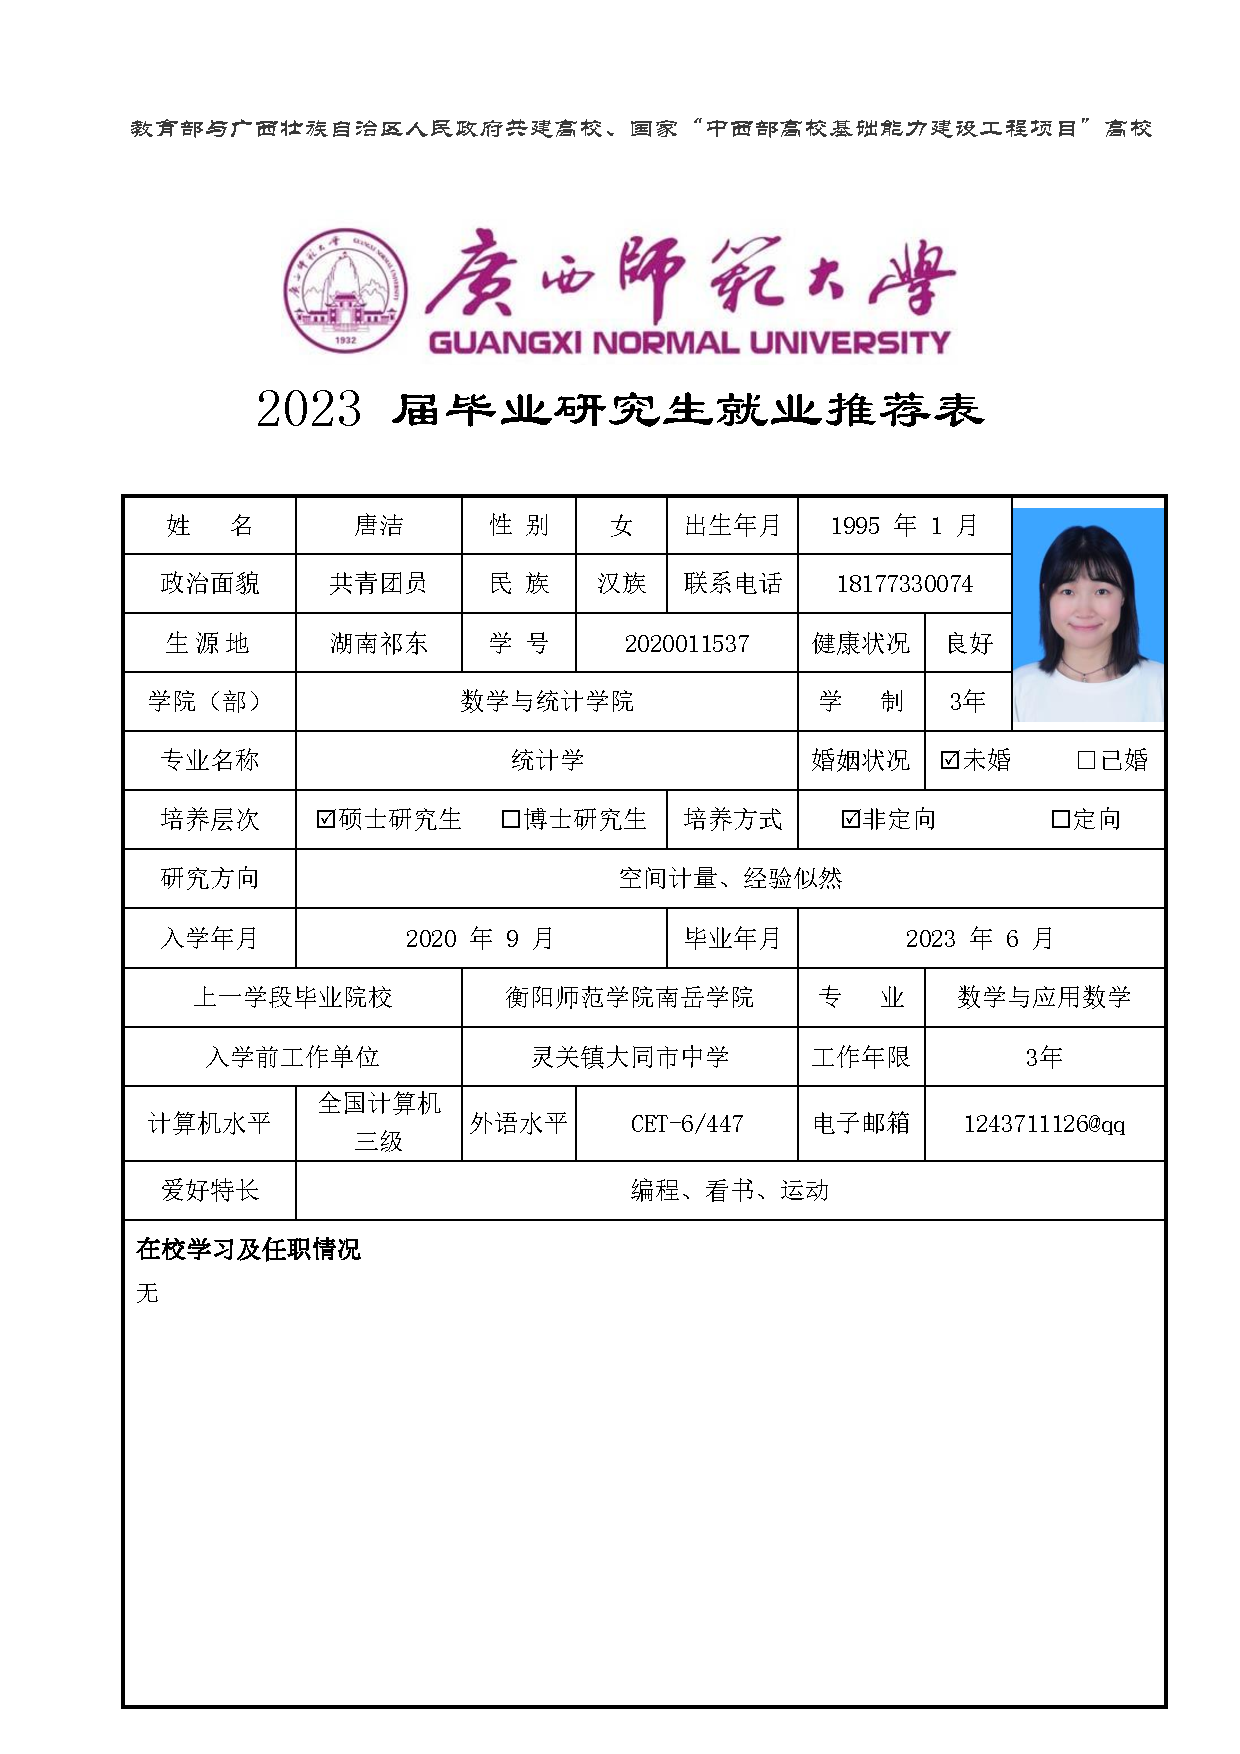
\includepdf[pages=1-4]{pdfs/硕士就业推荐表2.pdf}
%\begin{center}
%  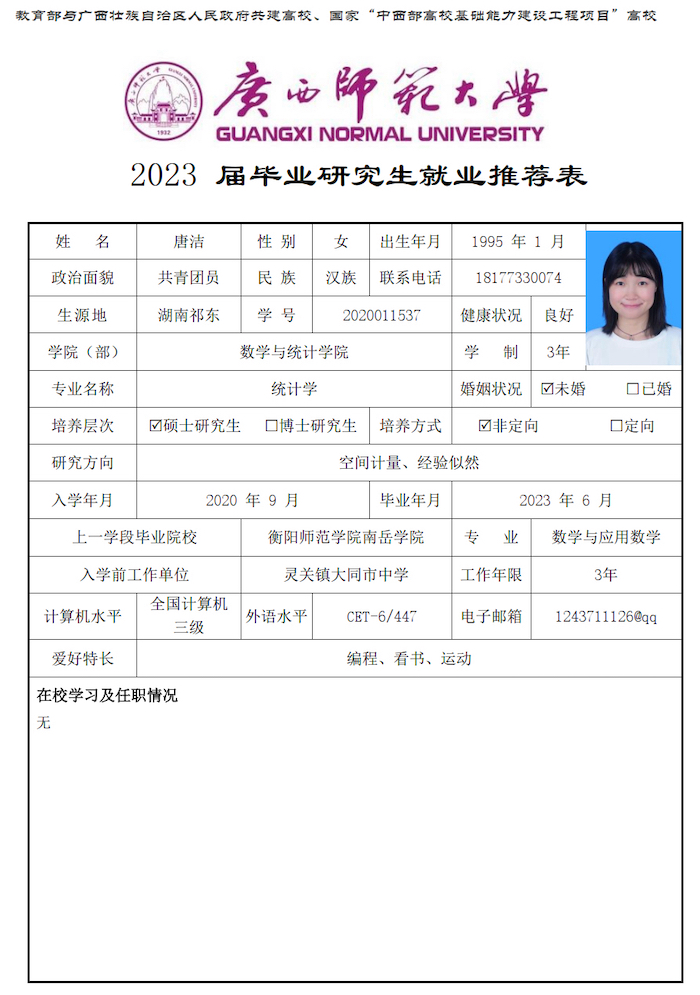
\includegraphics[scale=0.6]{figs/硕士就业推荐表1.jpg }
%  
%  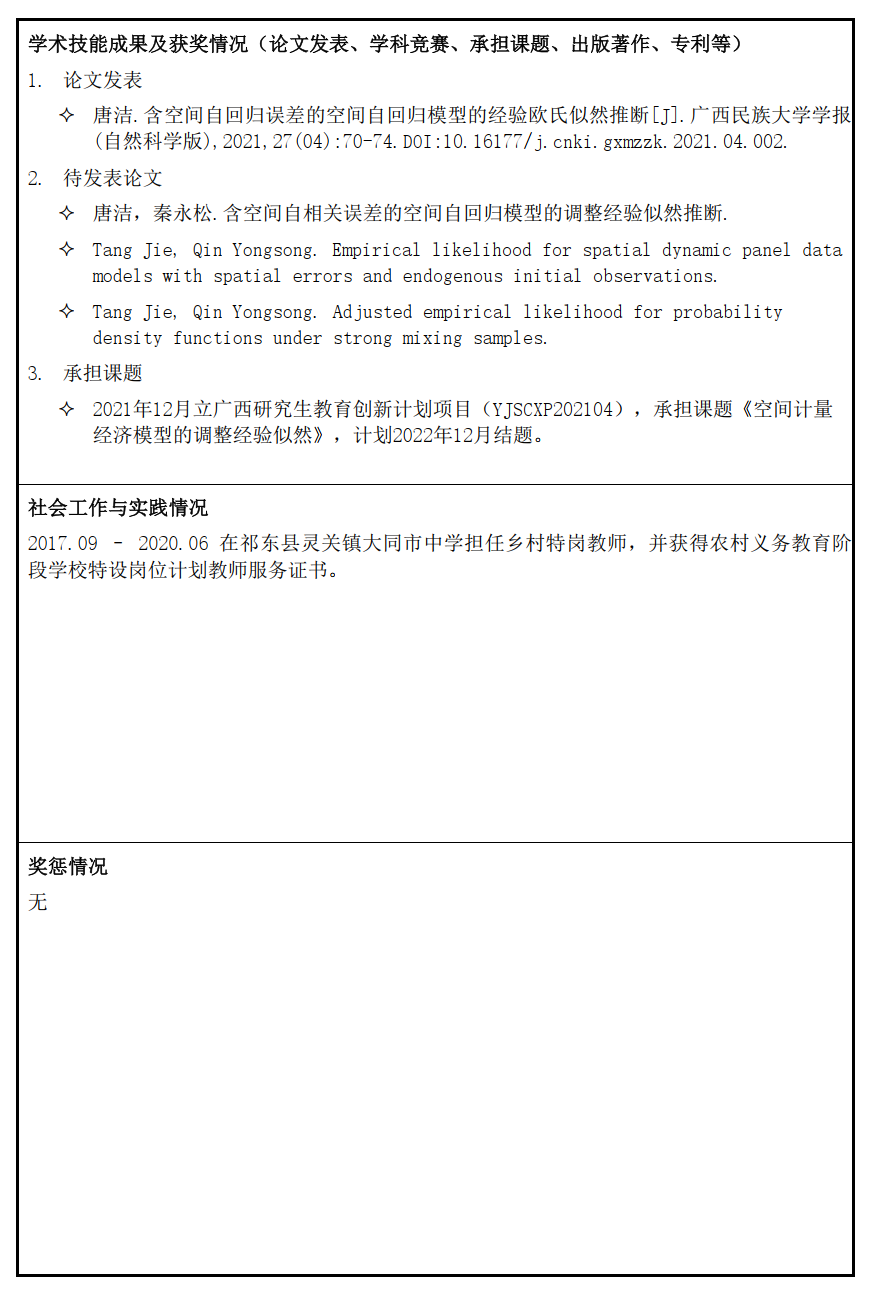
\includegraphics[scale=0.5]{figs/硕士就业推荐表2.jpg }
%  
%  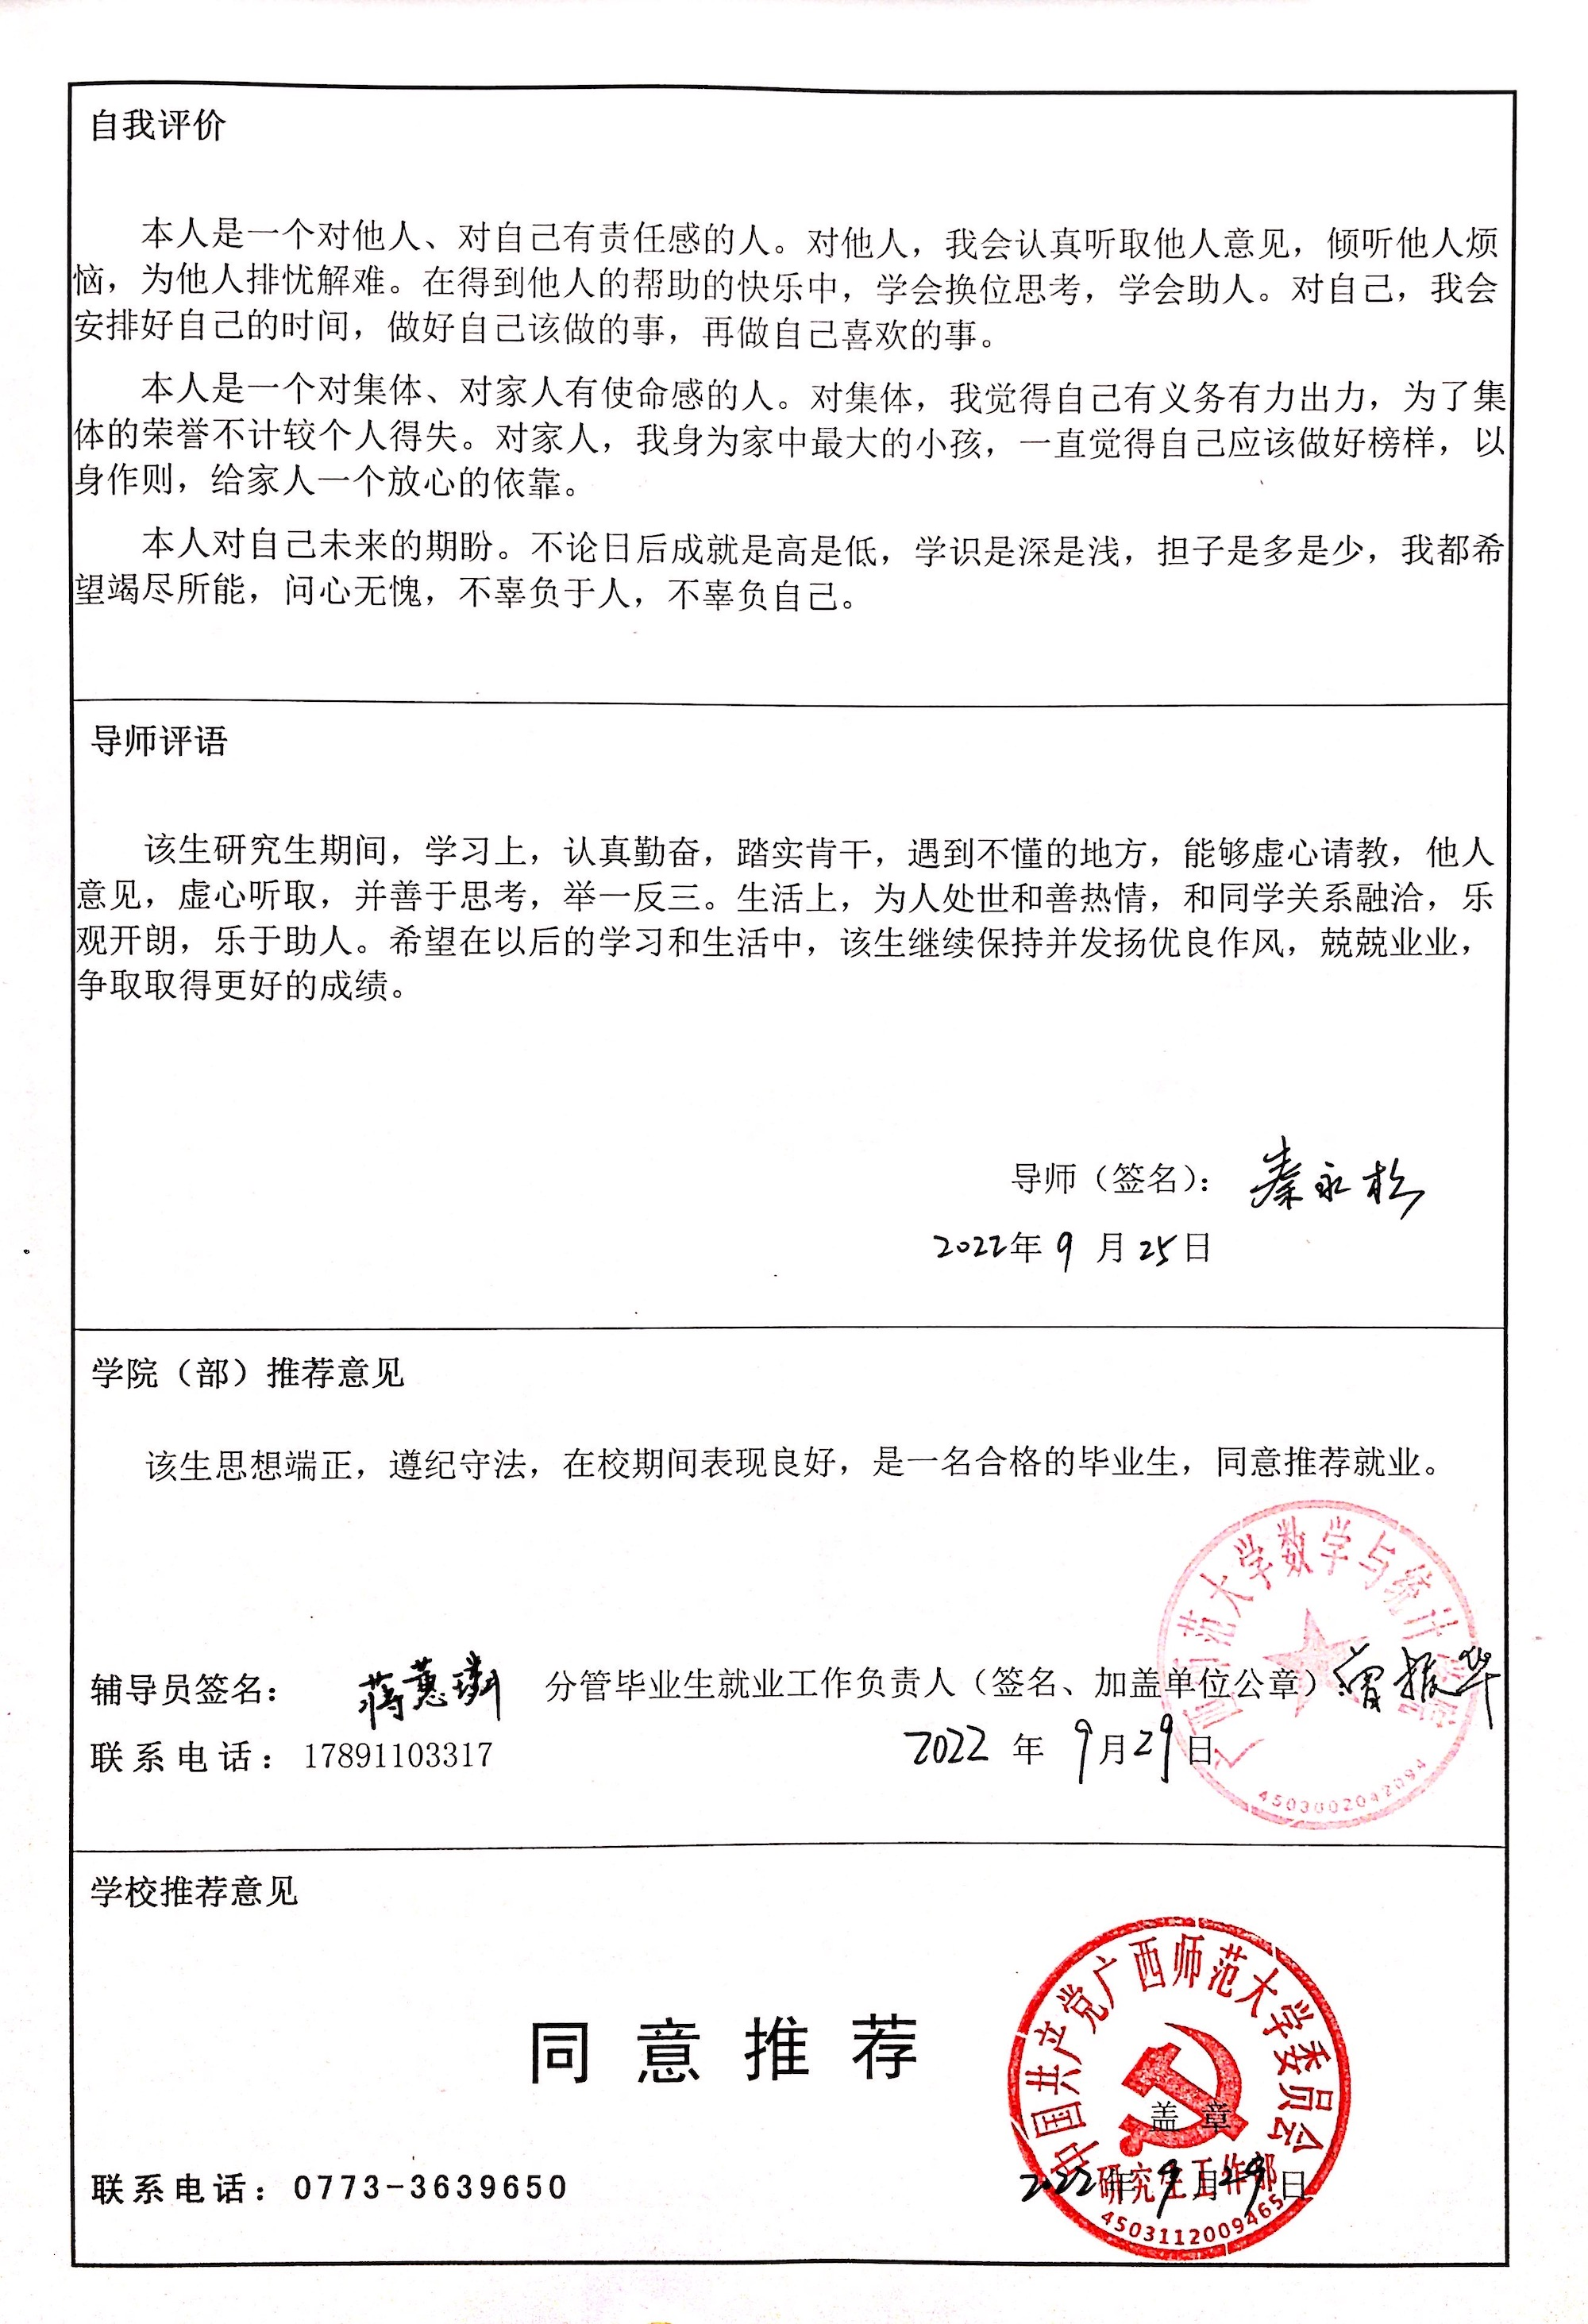
\includegraphics[scale=0.37]{figs/硕士就业推荐表4.jpg }
%\end{center}

%\section{学生证}
%\begin{center}
%  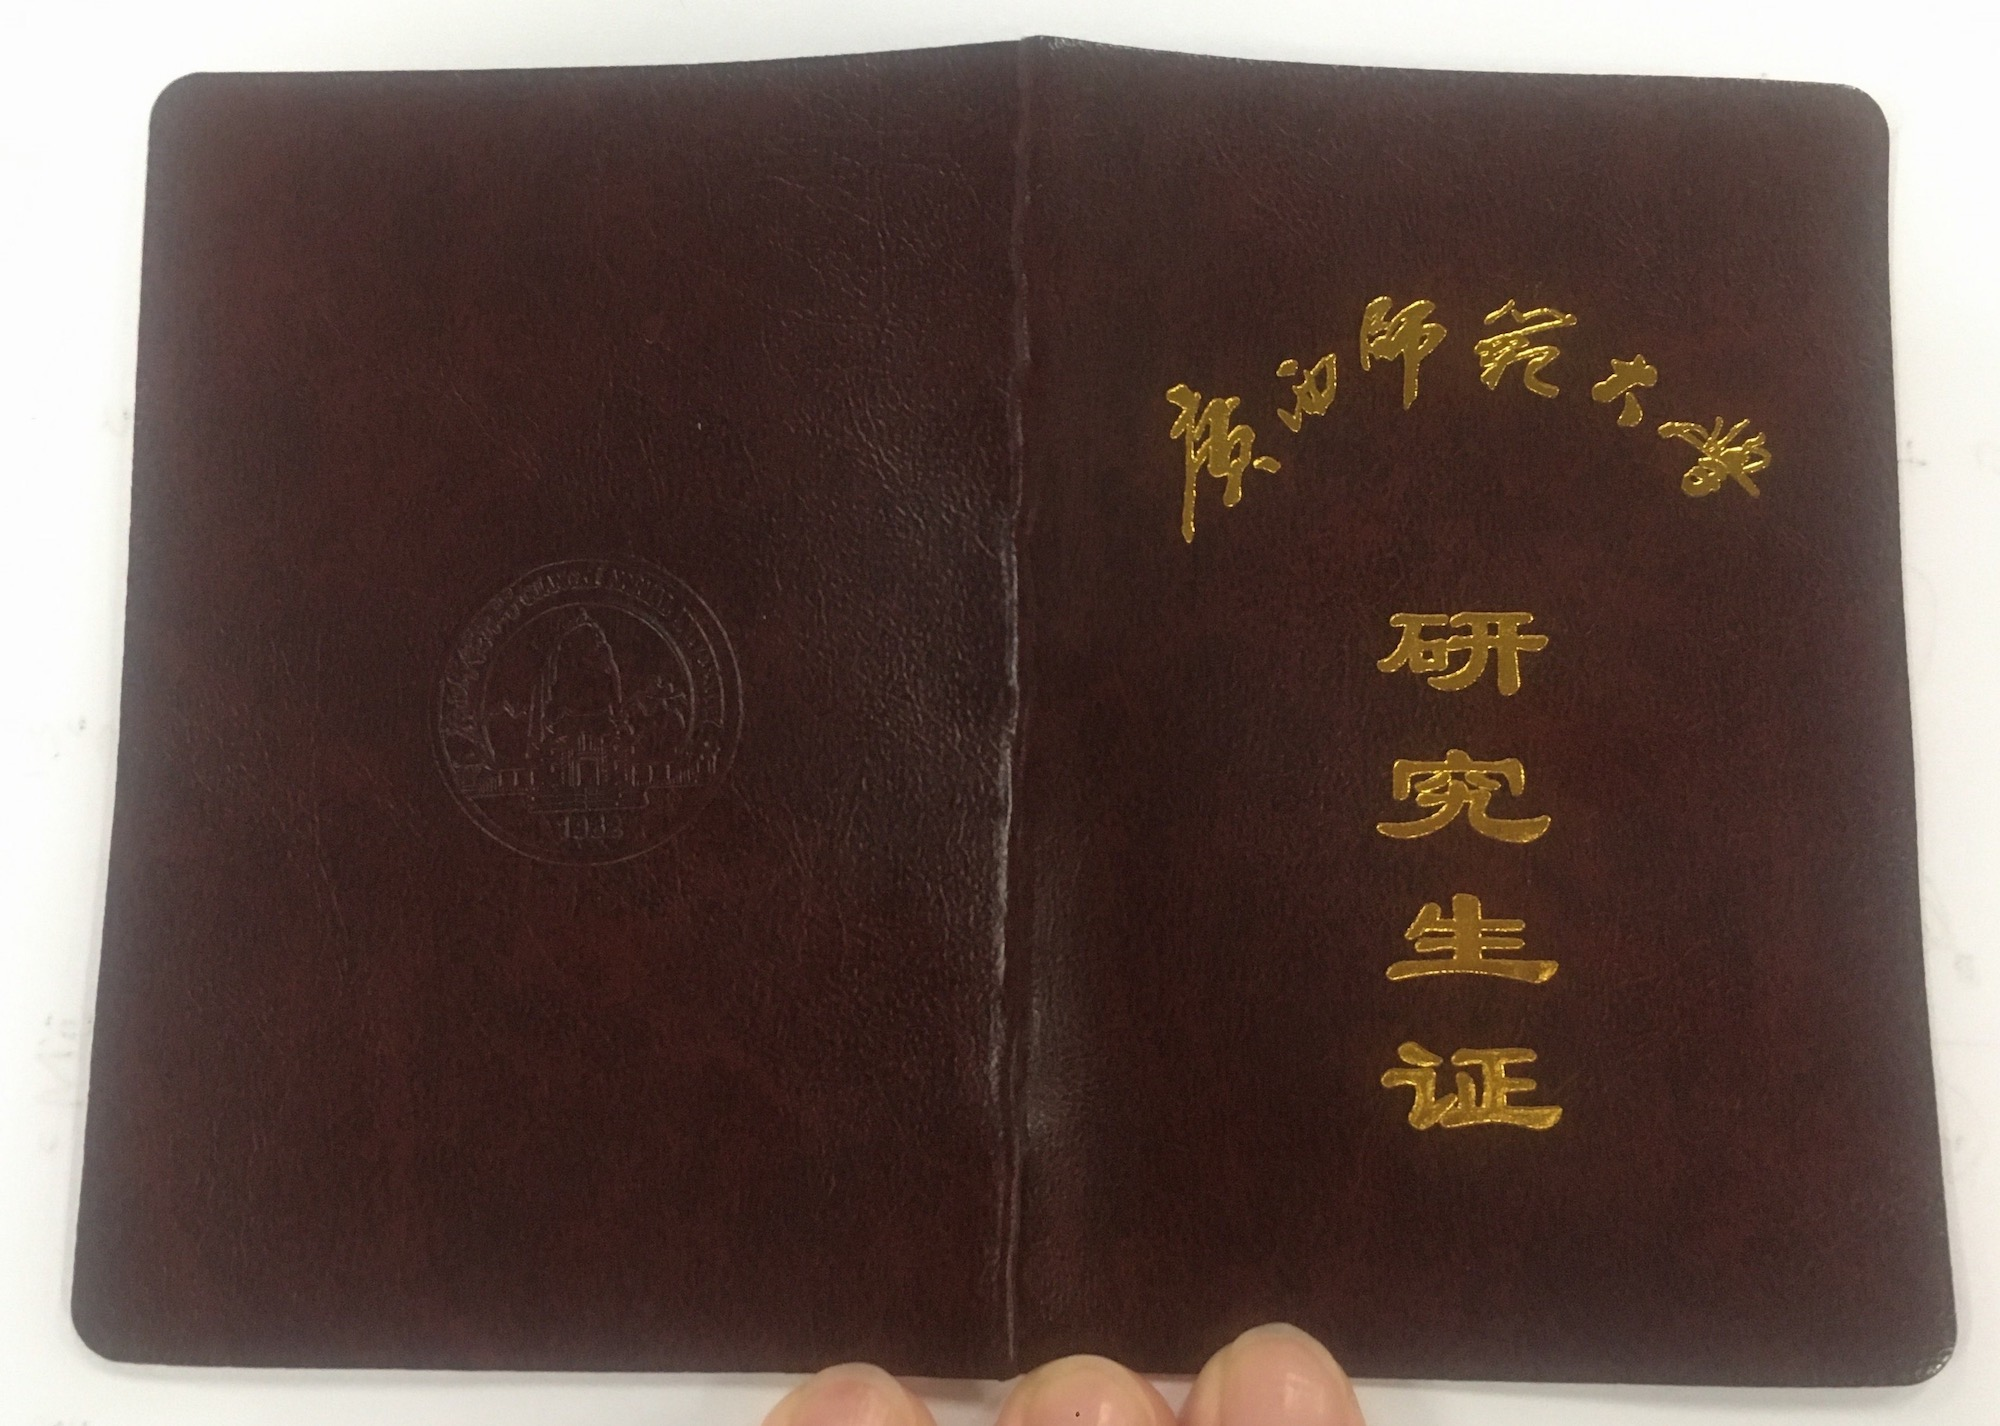
\includegraphics[scale=0.1]{figs/学生证1.jpg }
%  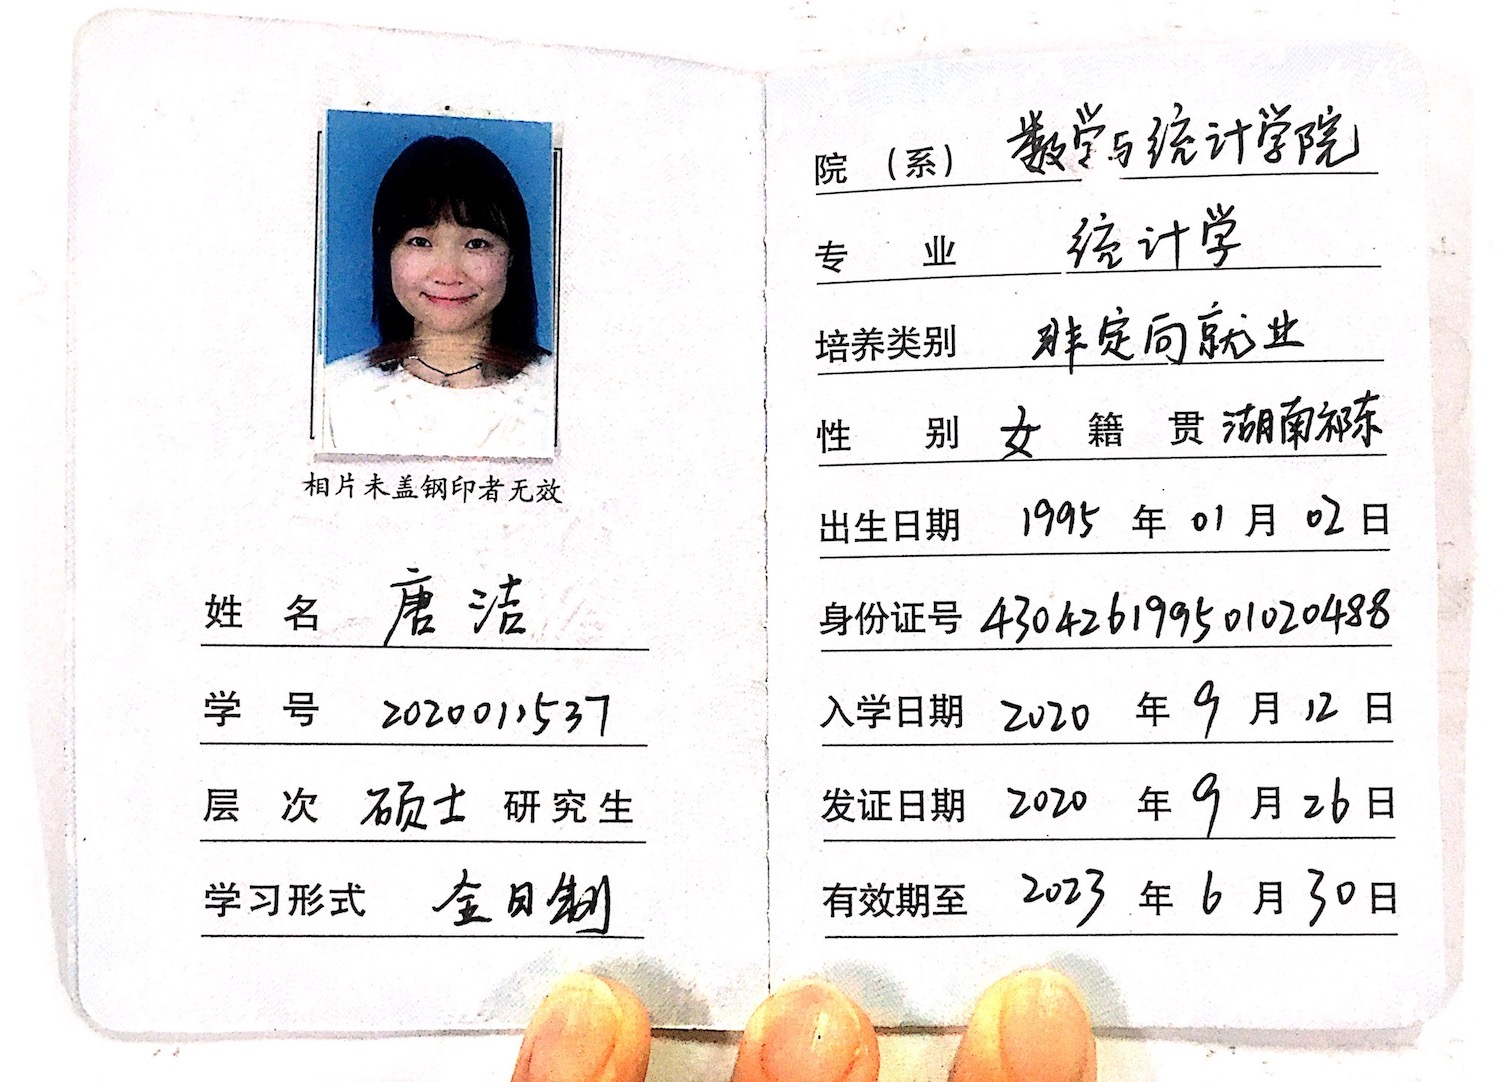
\includegraphics[scale=0.1]{figs/学生证2.jpg }
%  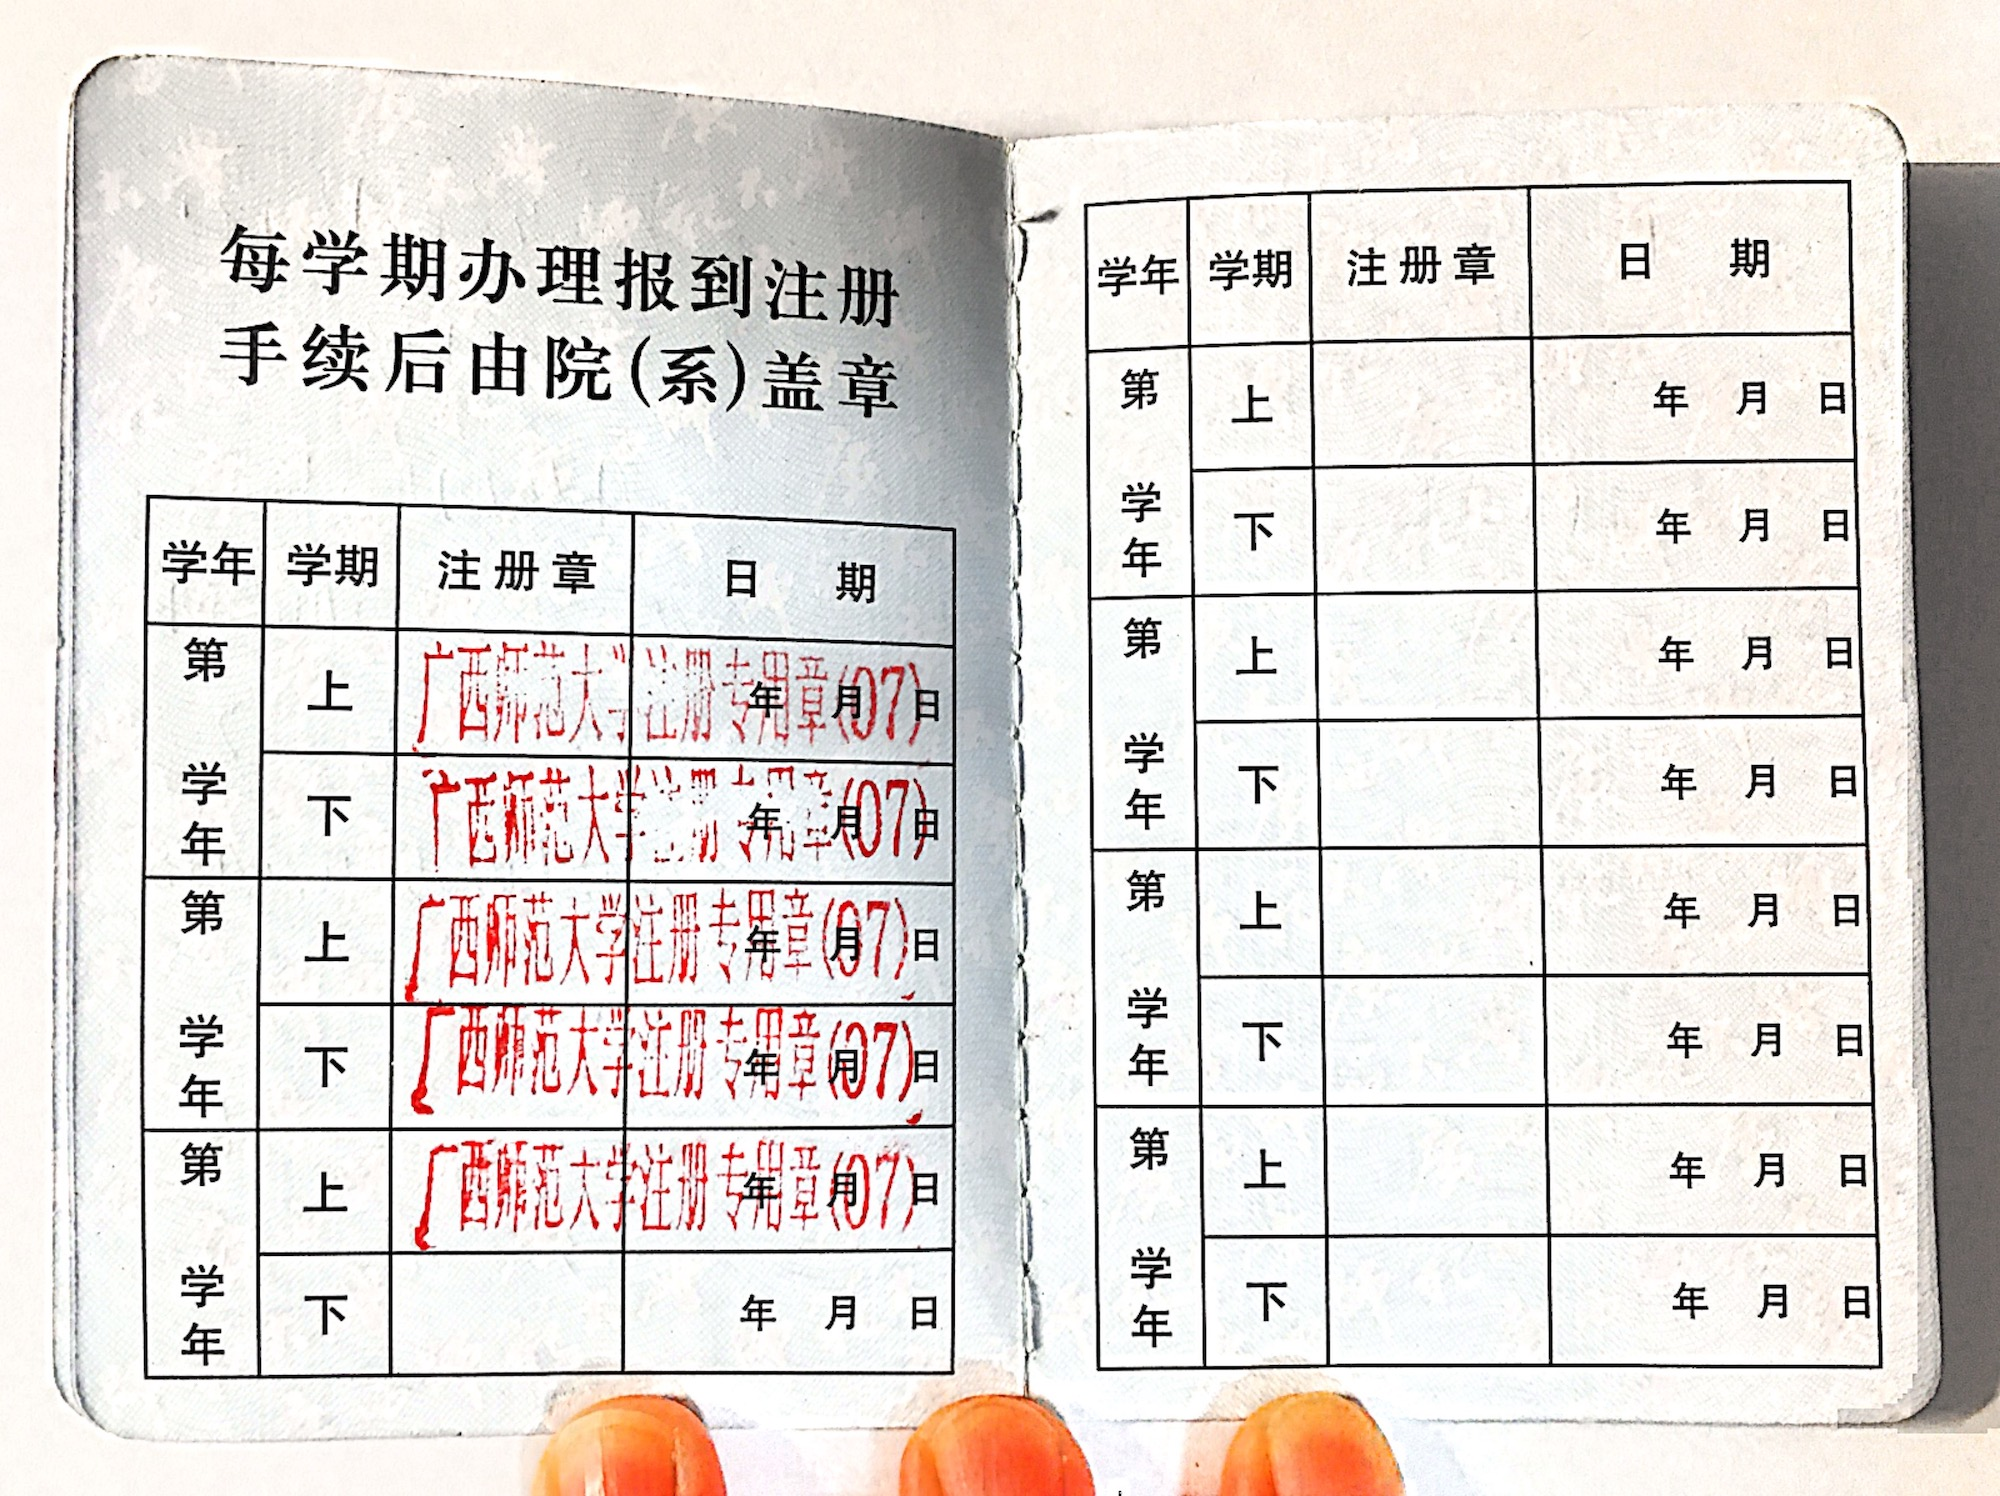
\includegraphics[scale=0.1]{figs/学生证3.jpg }
%\end{center}



\subsection{过级证书}
\subsubsection{职业资格证}
\begin{center}
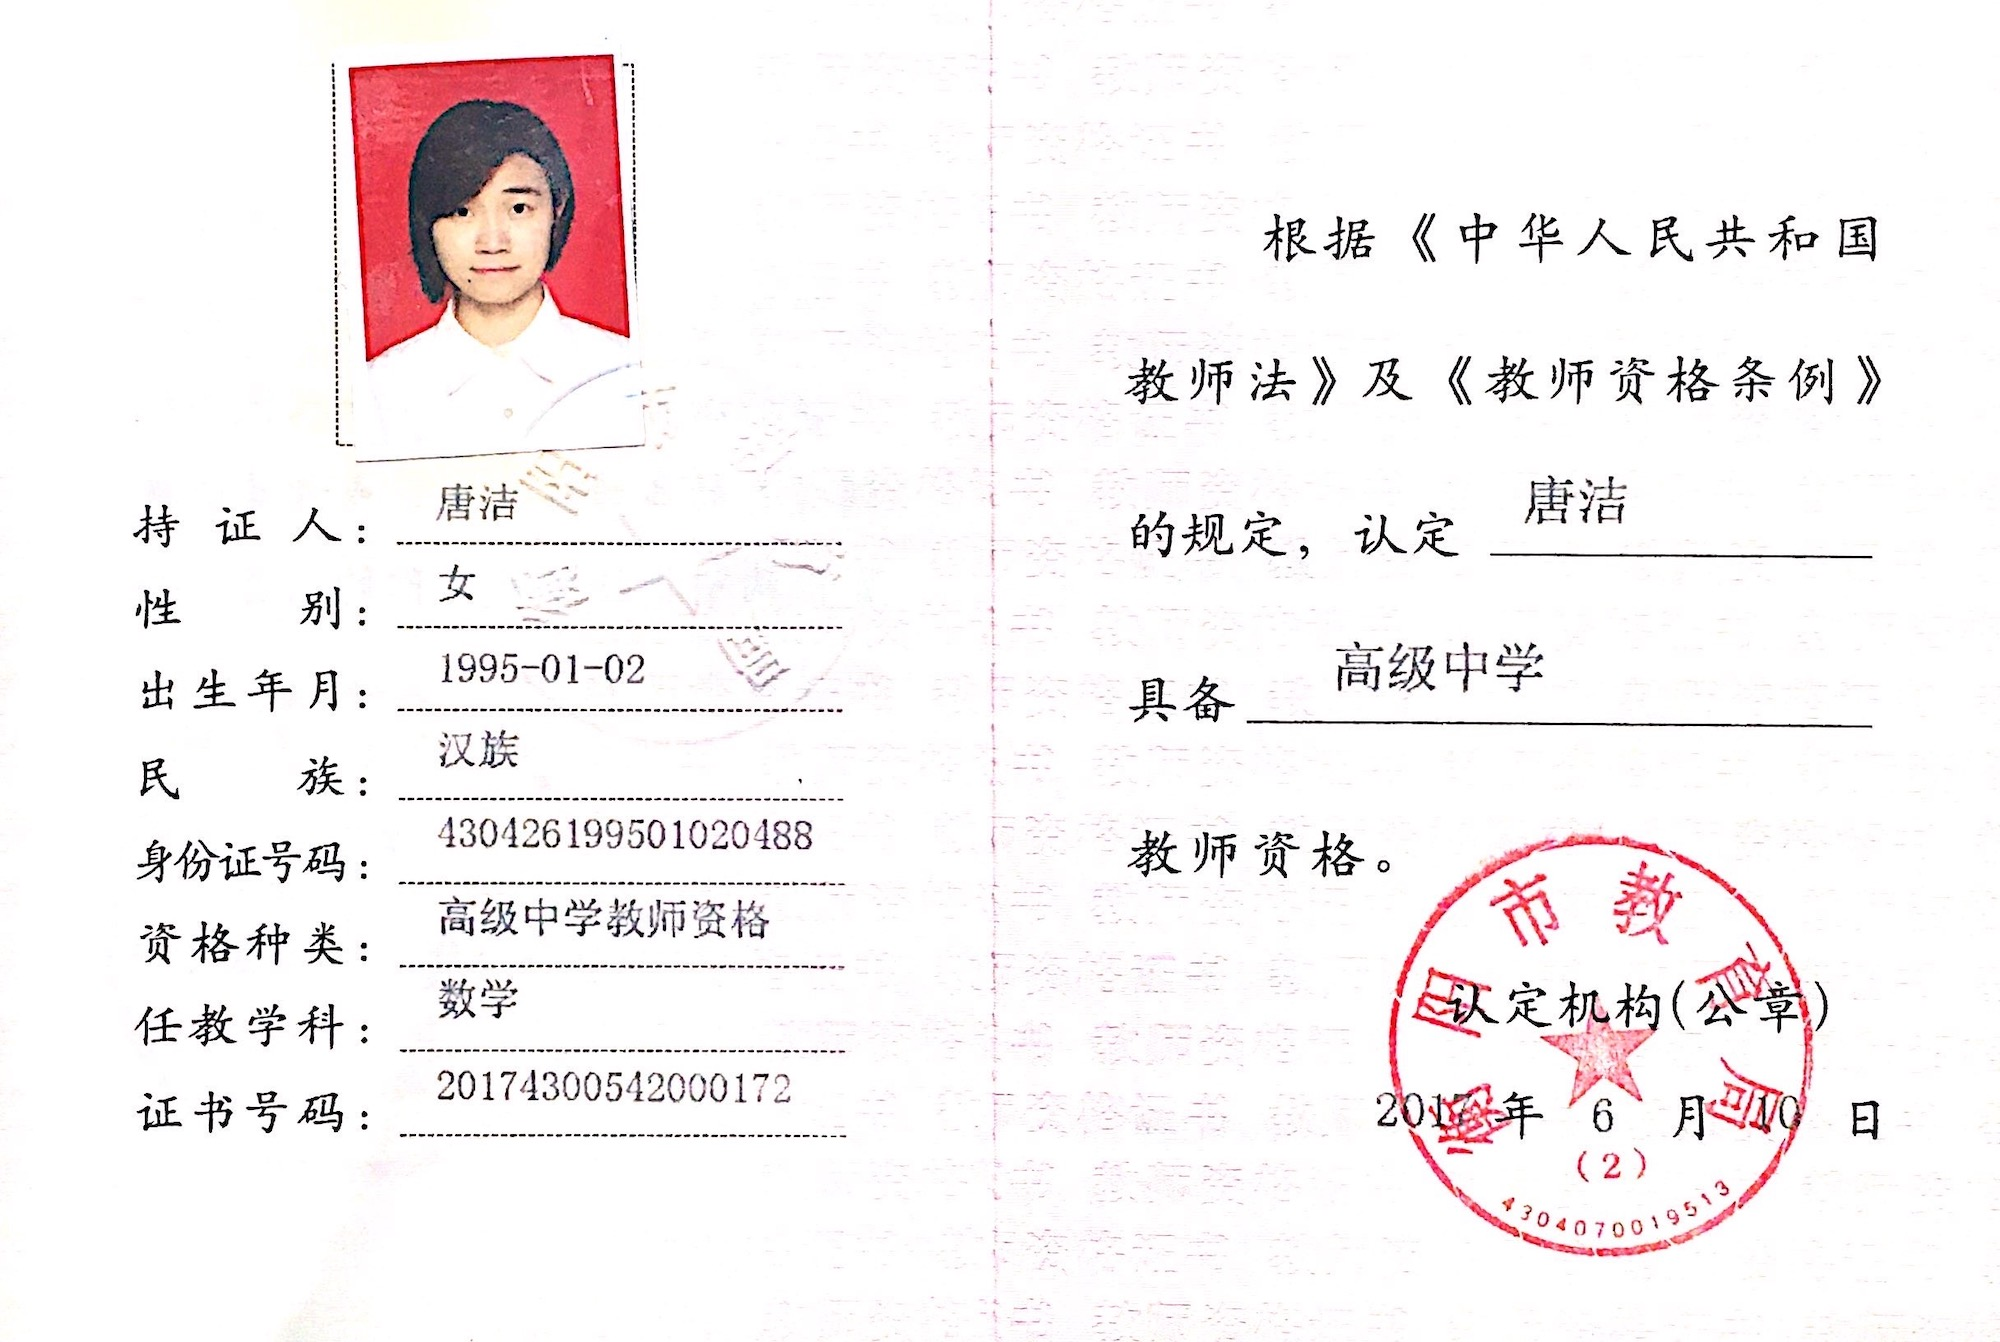
\includegraphics[scale=0.20]{figs/教师资格证.jpg }
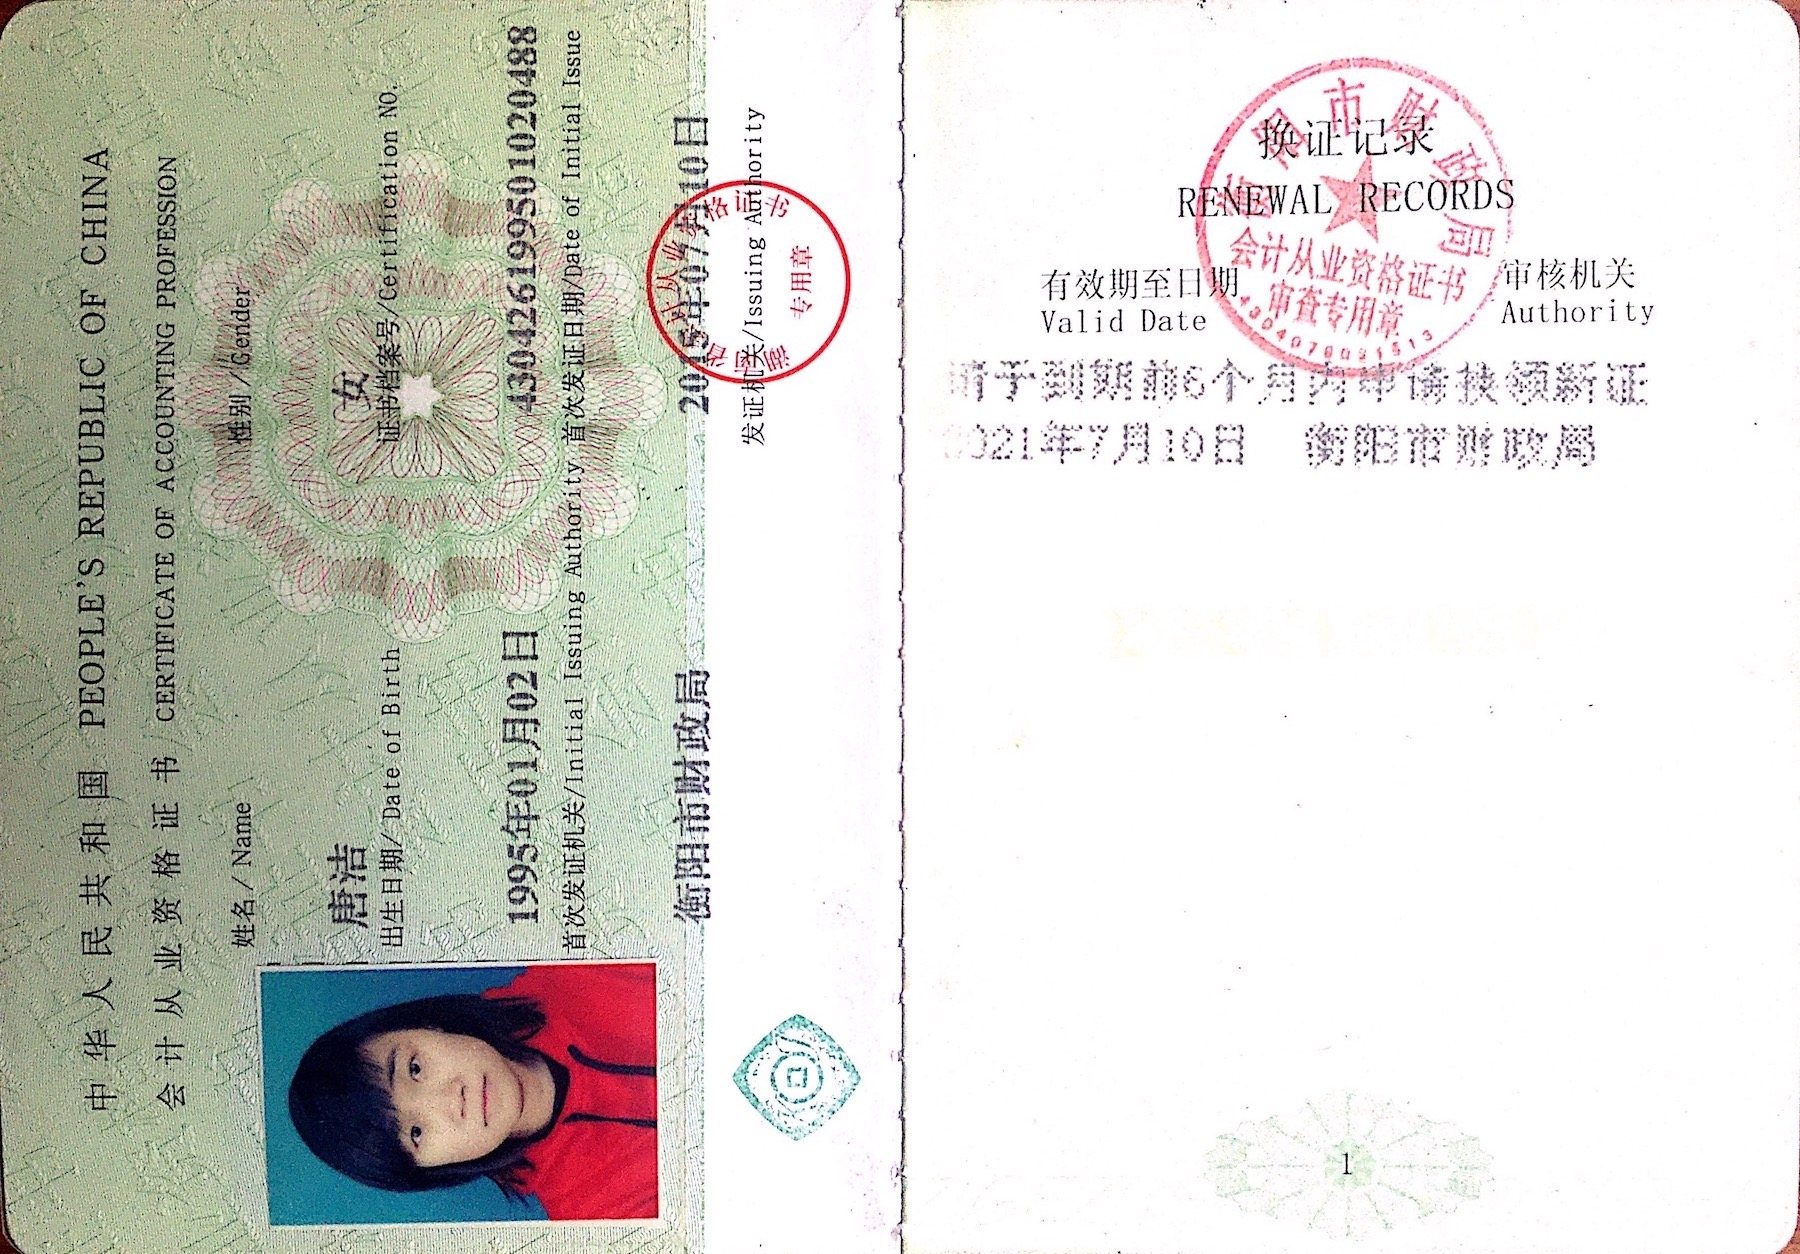
\includegraphics[scale=0.2]{figs/2015-07.jpg }
\end{center}

\subsubsection{职称证书}
\begin{center}
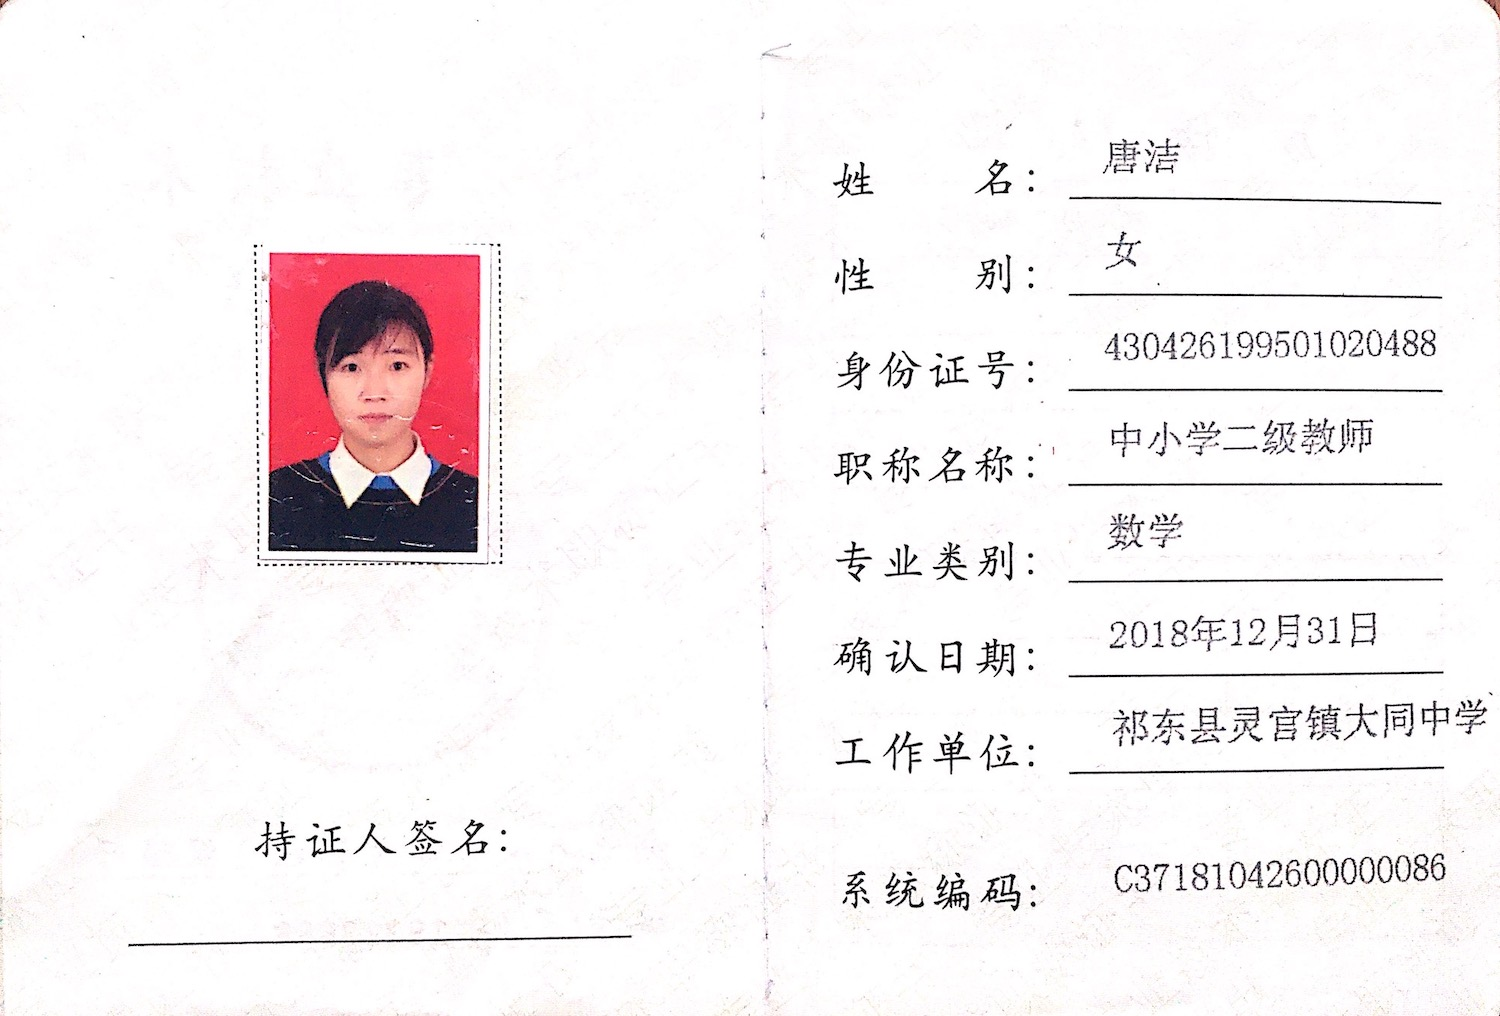
\includegraphics[scale=0.25]{figs/中二职称证书.jpg }
 \end{center}
 
\subsubsection{计算机等级证}
\begin{center}
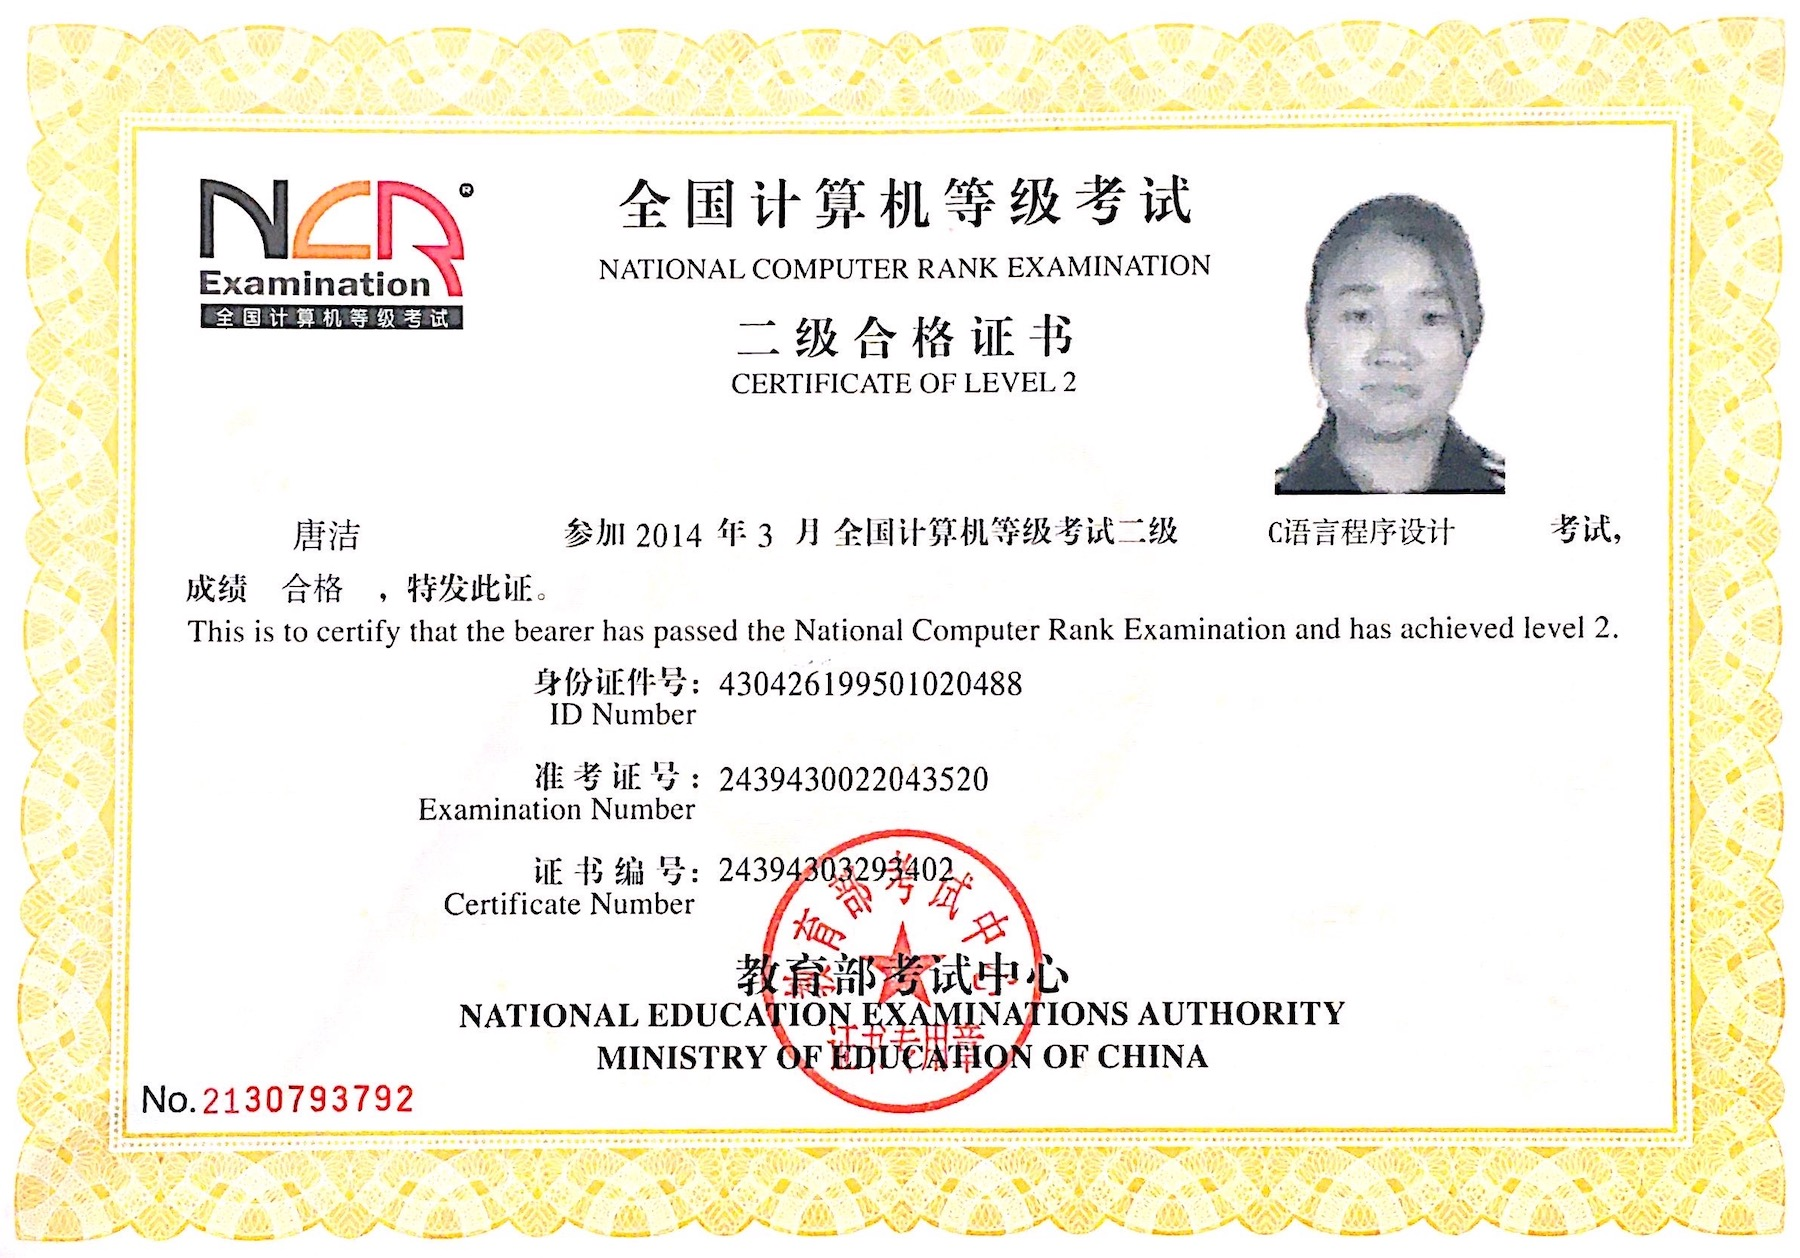
\includegraphics[scale=0.22]{figs/计算机二级C.jpg }
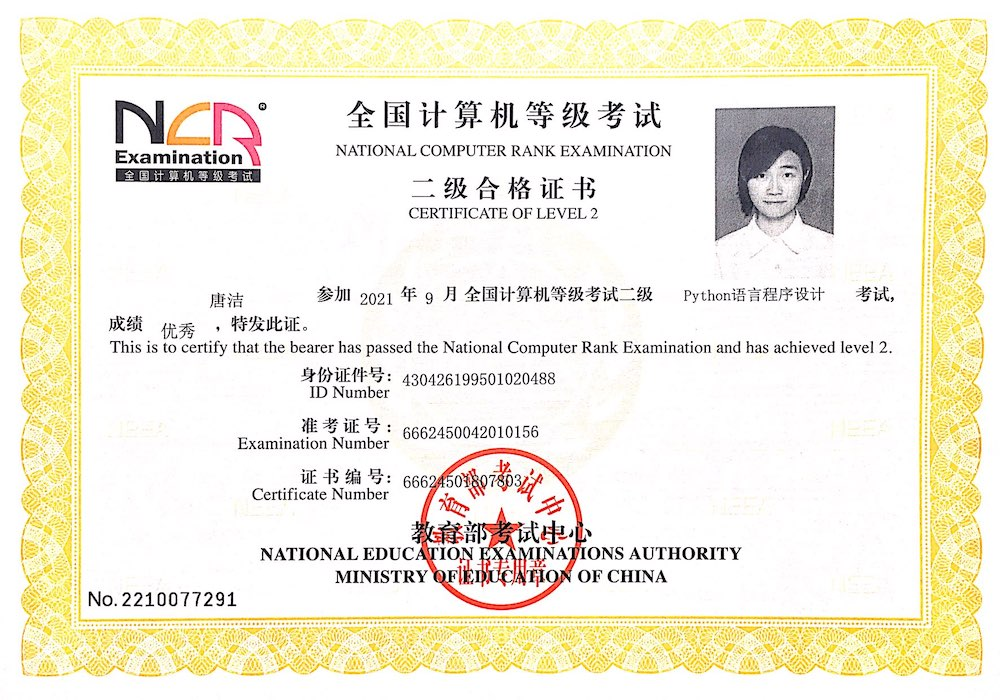
\includegraphics[scale=0.4]{figs/计算机二级Python.jpg }
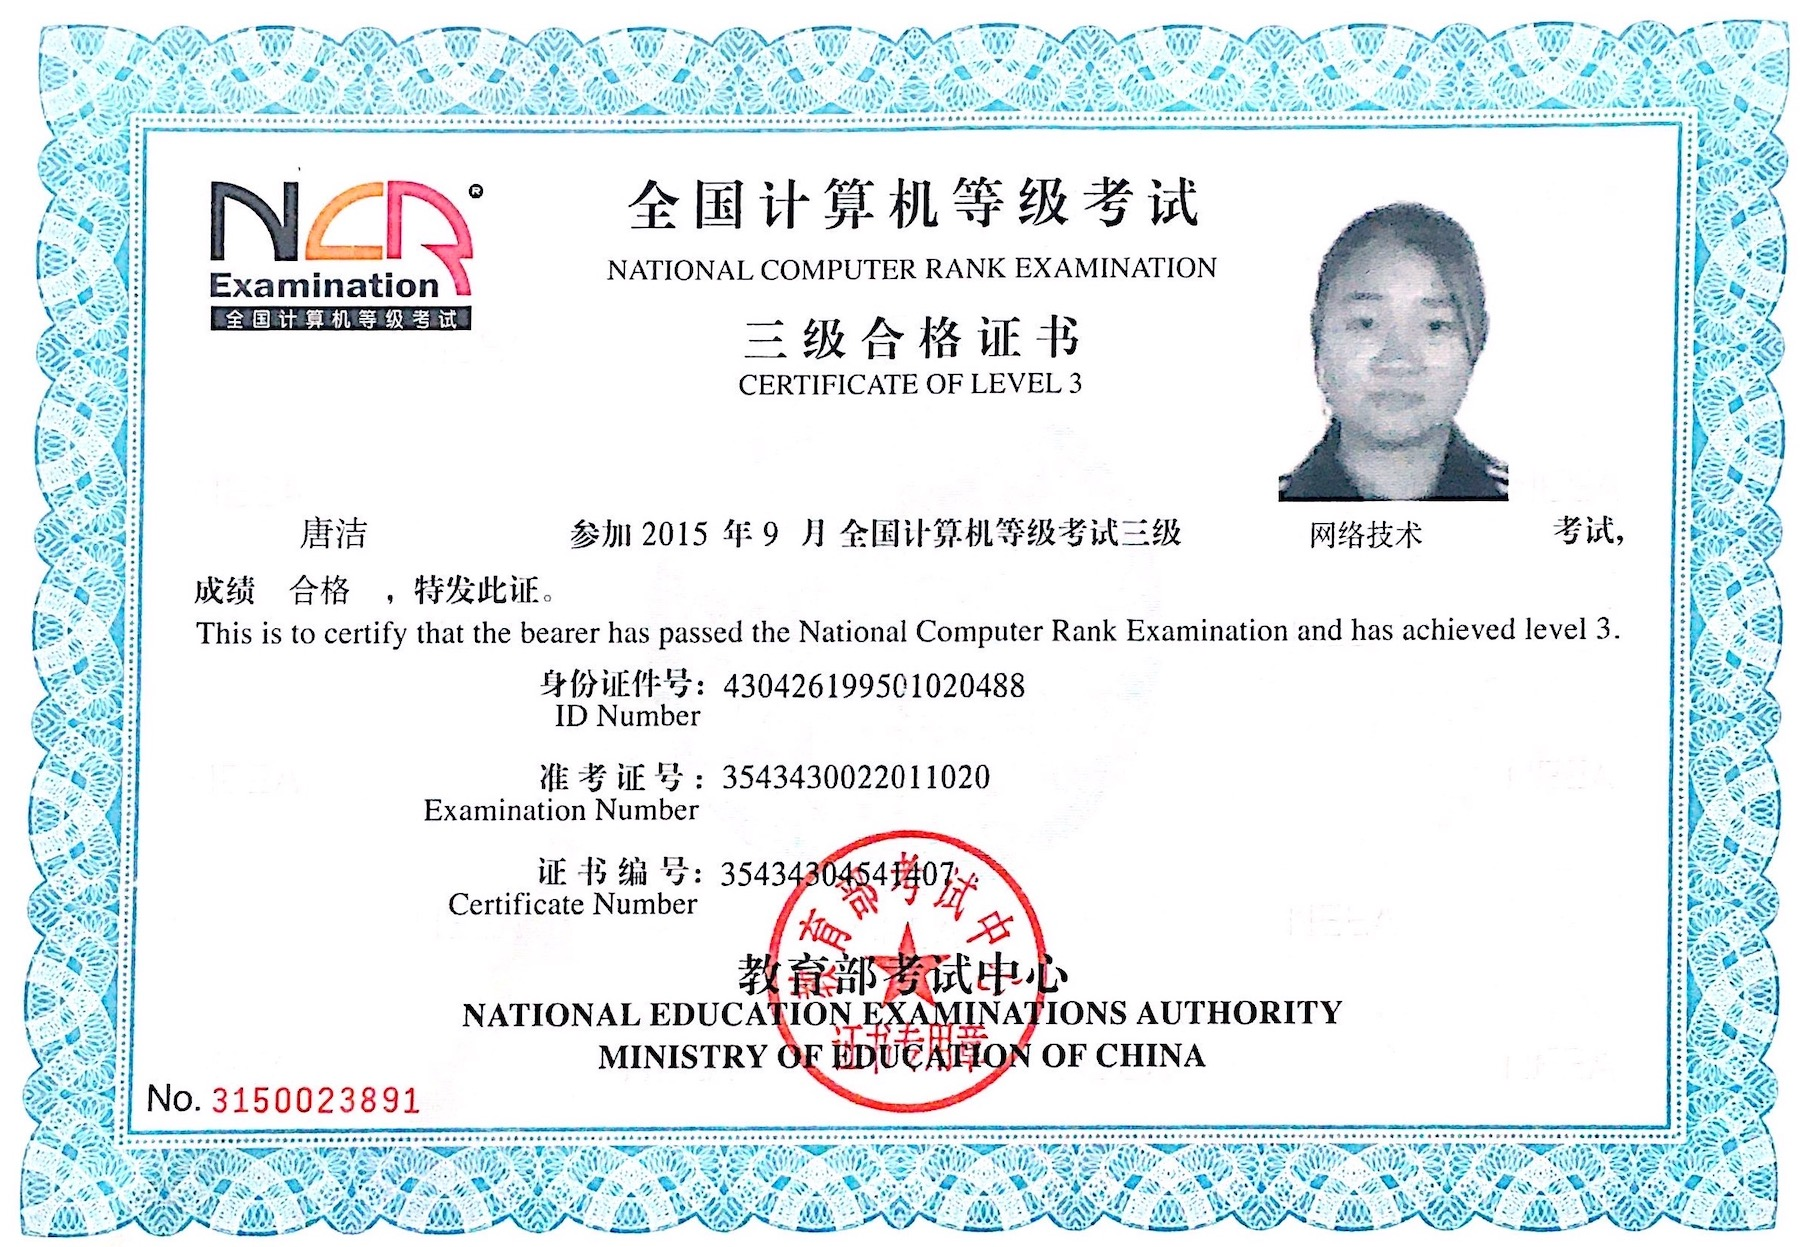
\includegraphics[scale=0.22]{figs/计算机三级证书.jpg }
\end{center}
 
\subsubsection{普通话证}
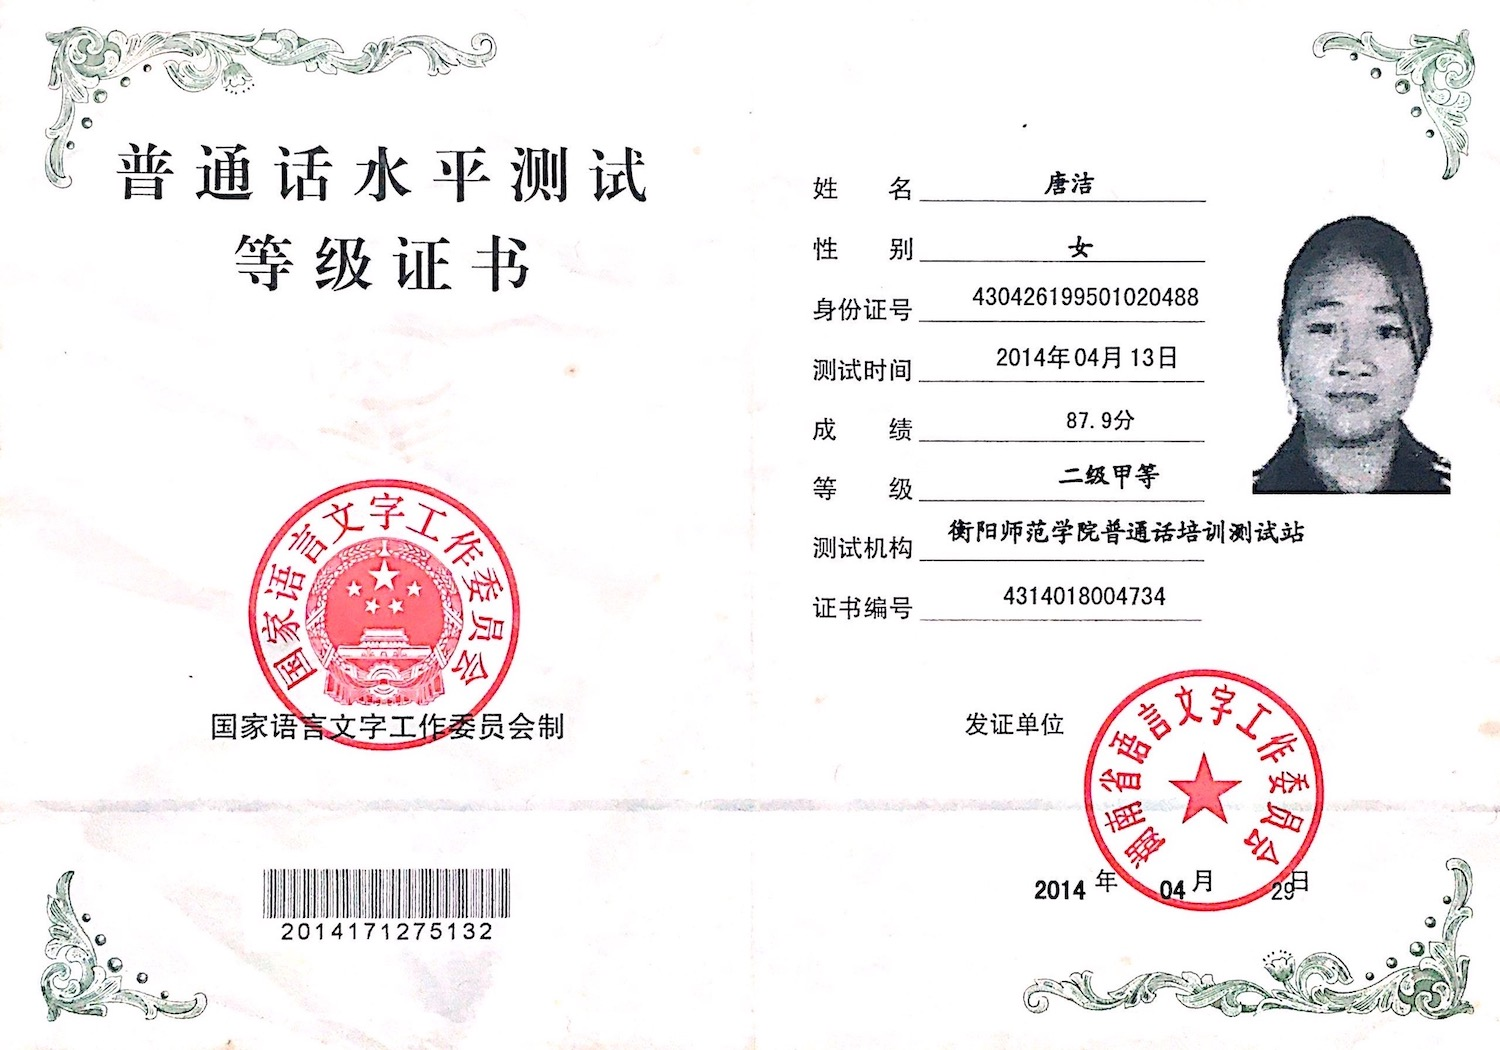
\includegraphics[scale=0.25]{figs/普通话证.jpg }

\subsubsection{英语六级}

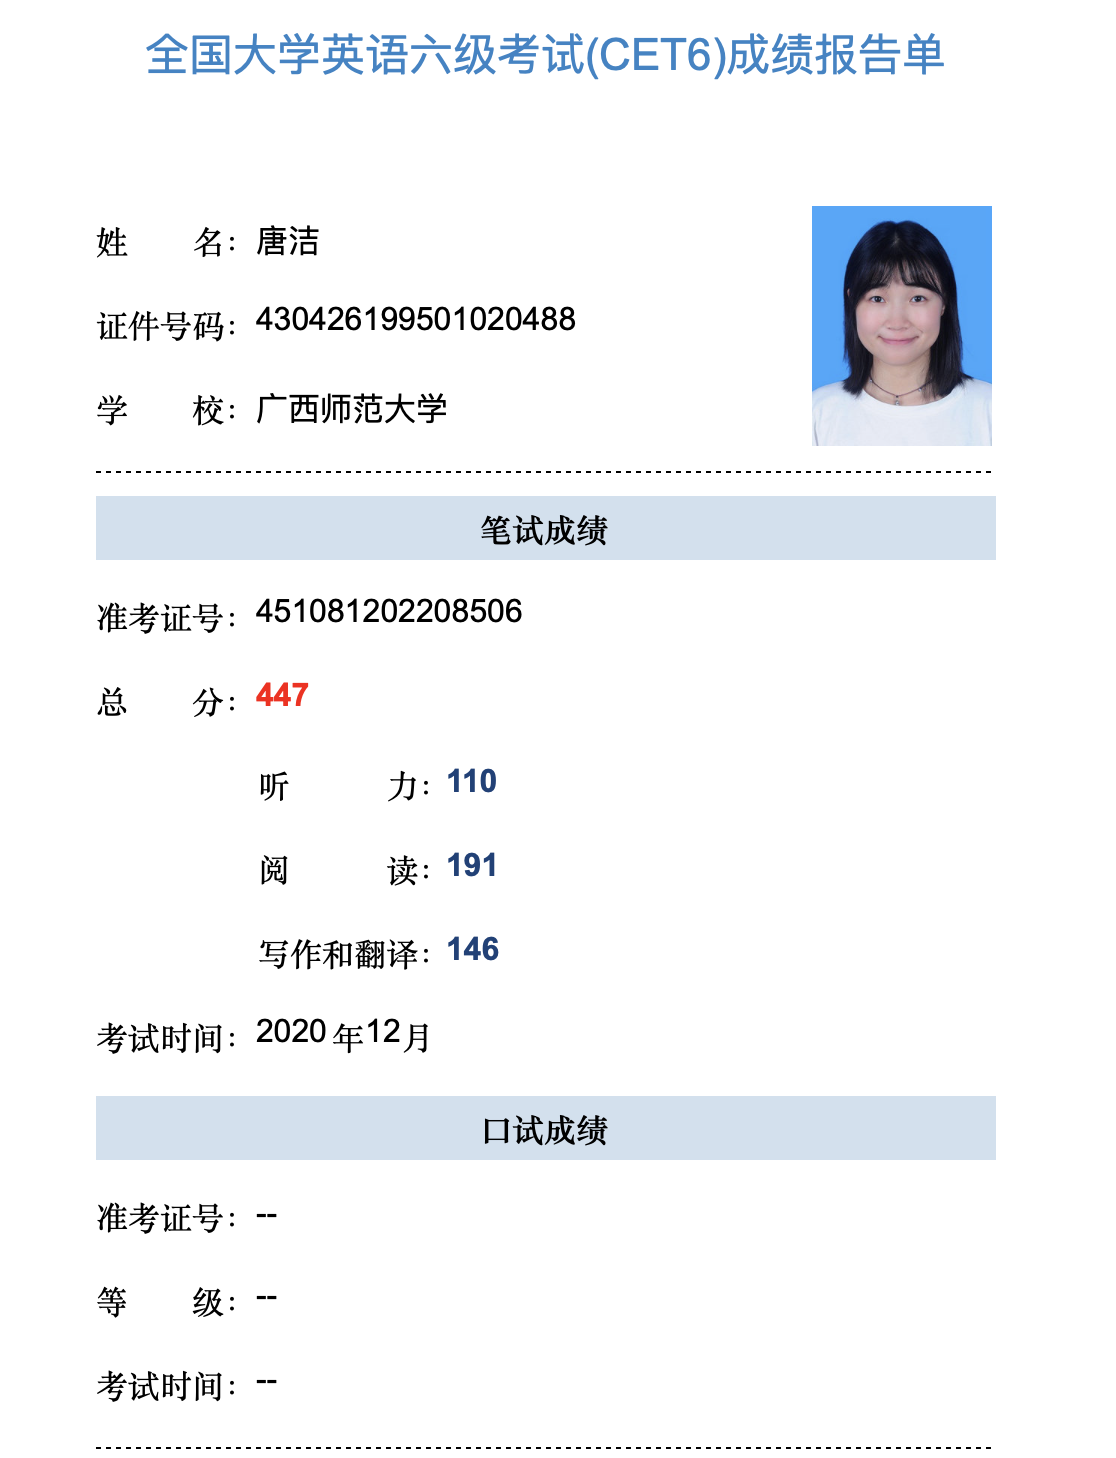
\includegraphics[scale=0.3]{figs/英语六级.jpg }



\subsection{荣誉证书}
\begin{center}
 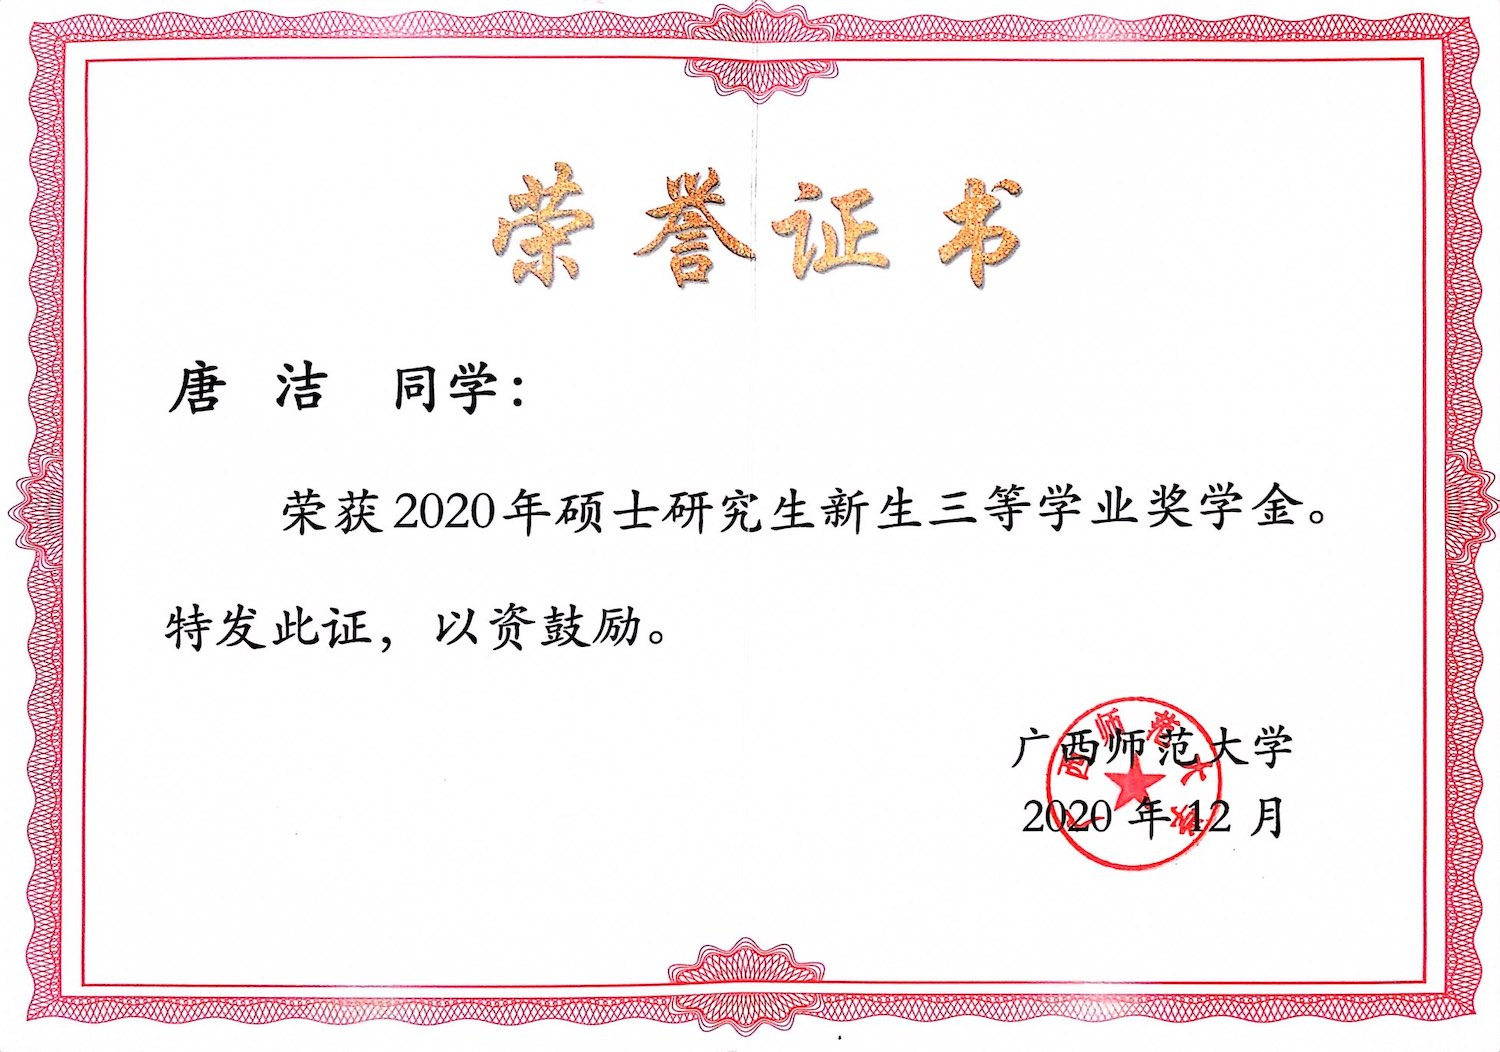
\includegraphics[scale=0.22]{figs/2020-12.jpg }
  
\includegraphics[scale=0.15]{figs/2021-12.jpg }
 
\includegraphics[scale=0.15]{figs/2022-12.jpg }
 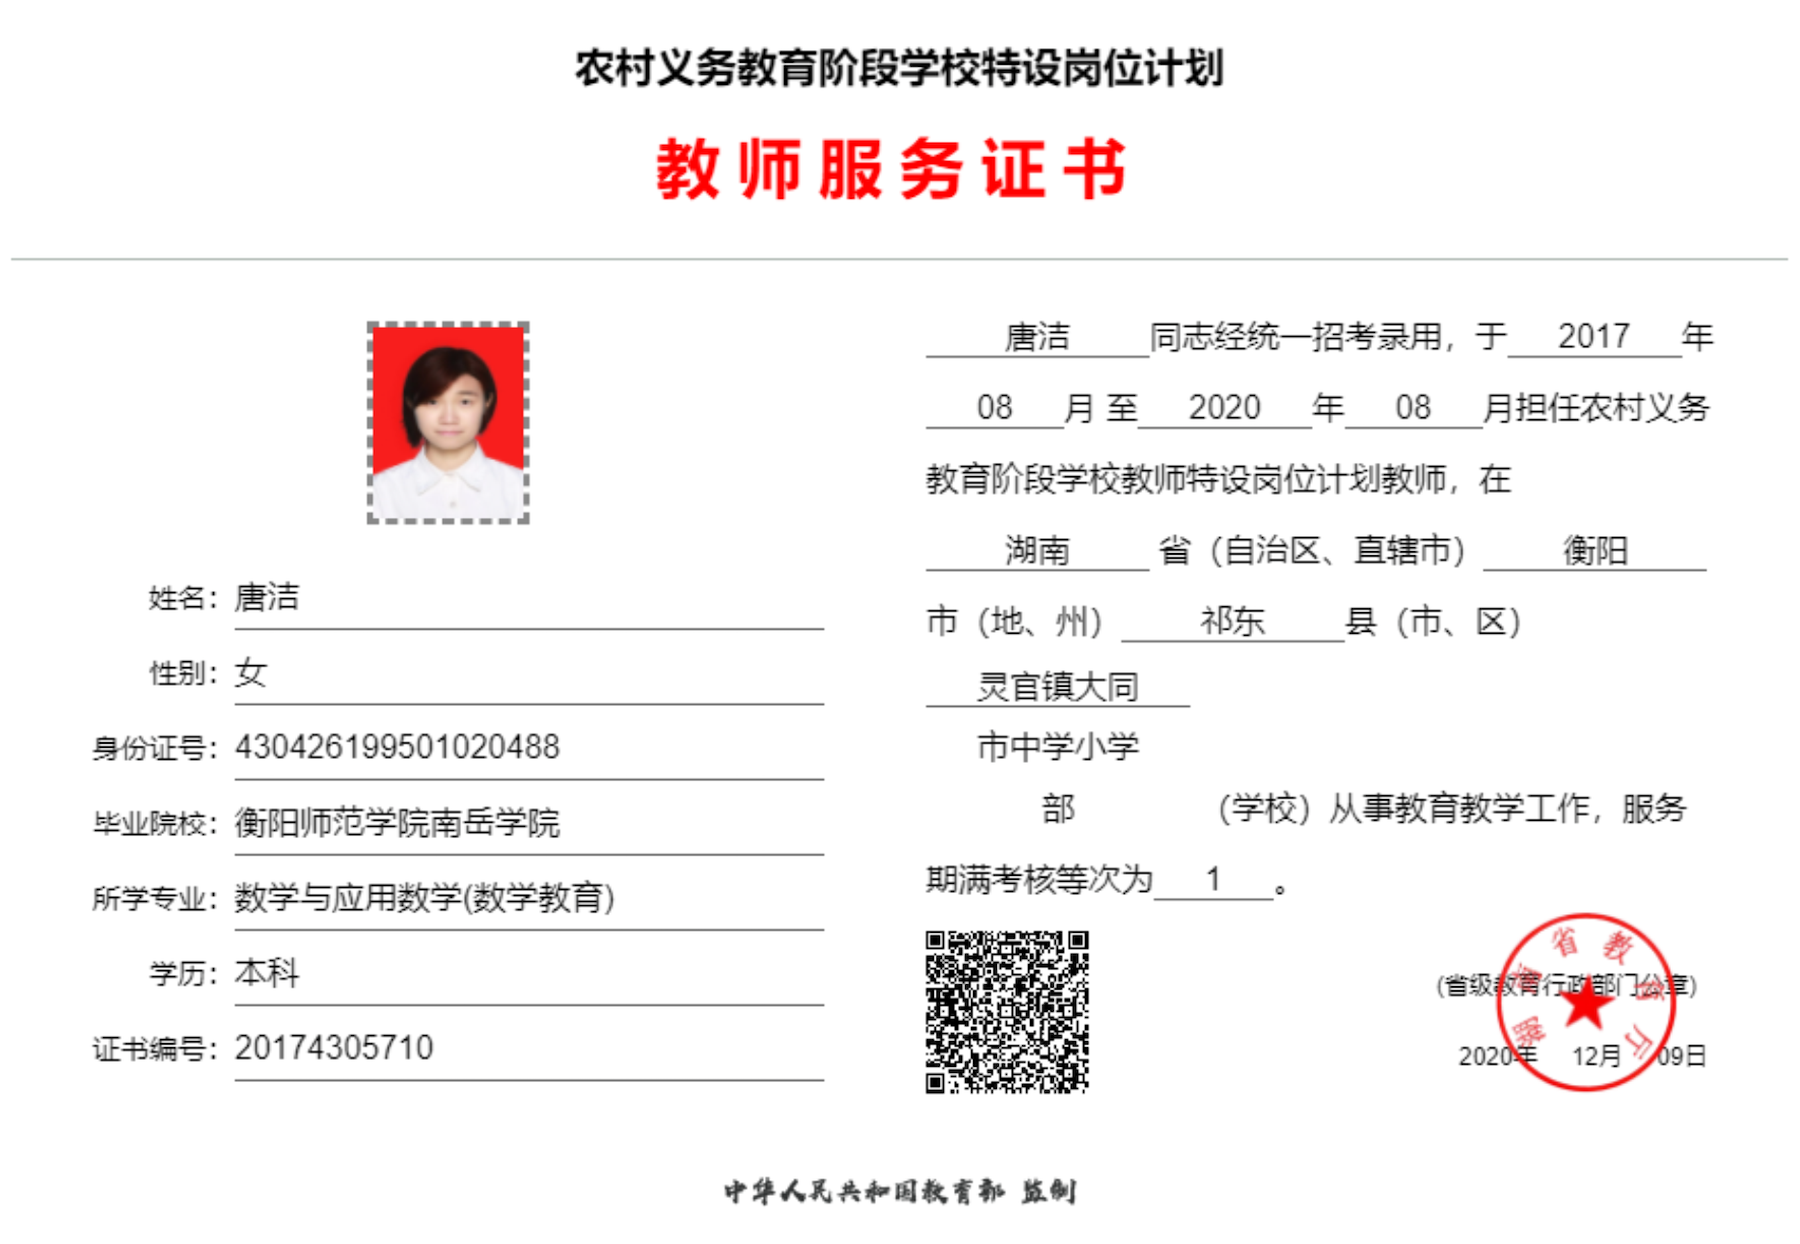
\includegraphics[scale=0.2]{figs/特岗服务证书.jpg }
 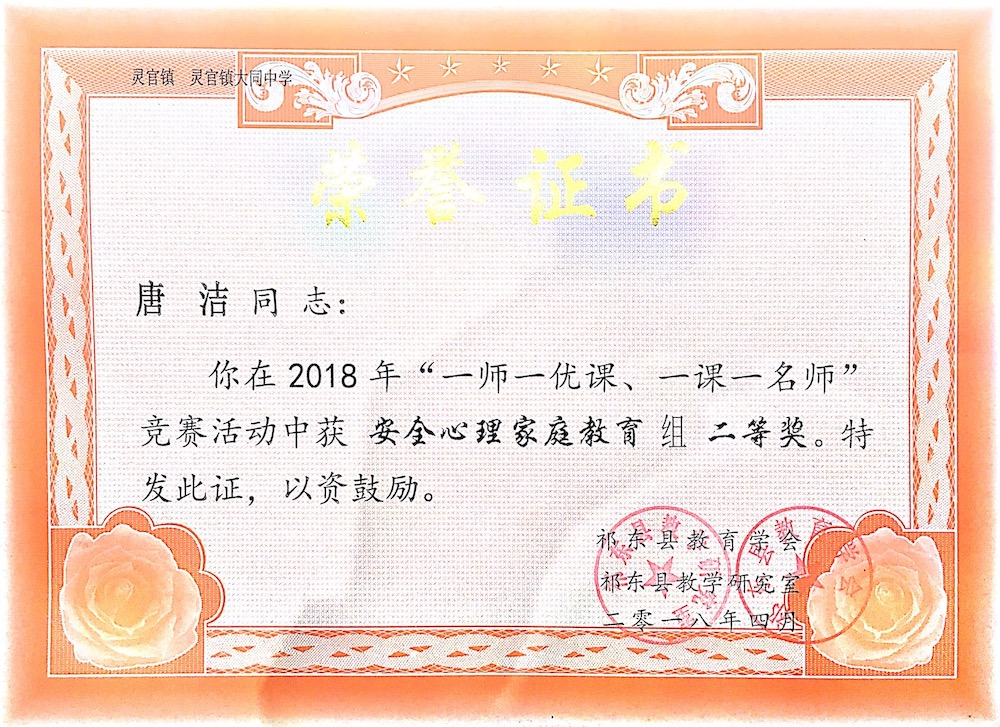
\includegraphics[scale=0.37]{figs/2018-04.jpg }
 
\includegraphics[scale=0.25]{figs/2018-05.jpg }
 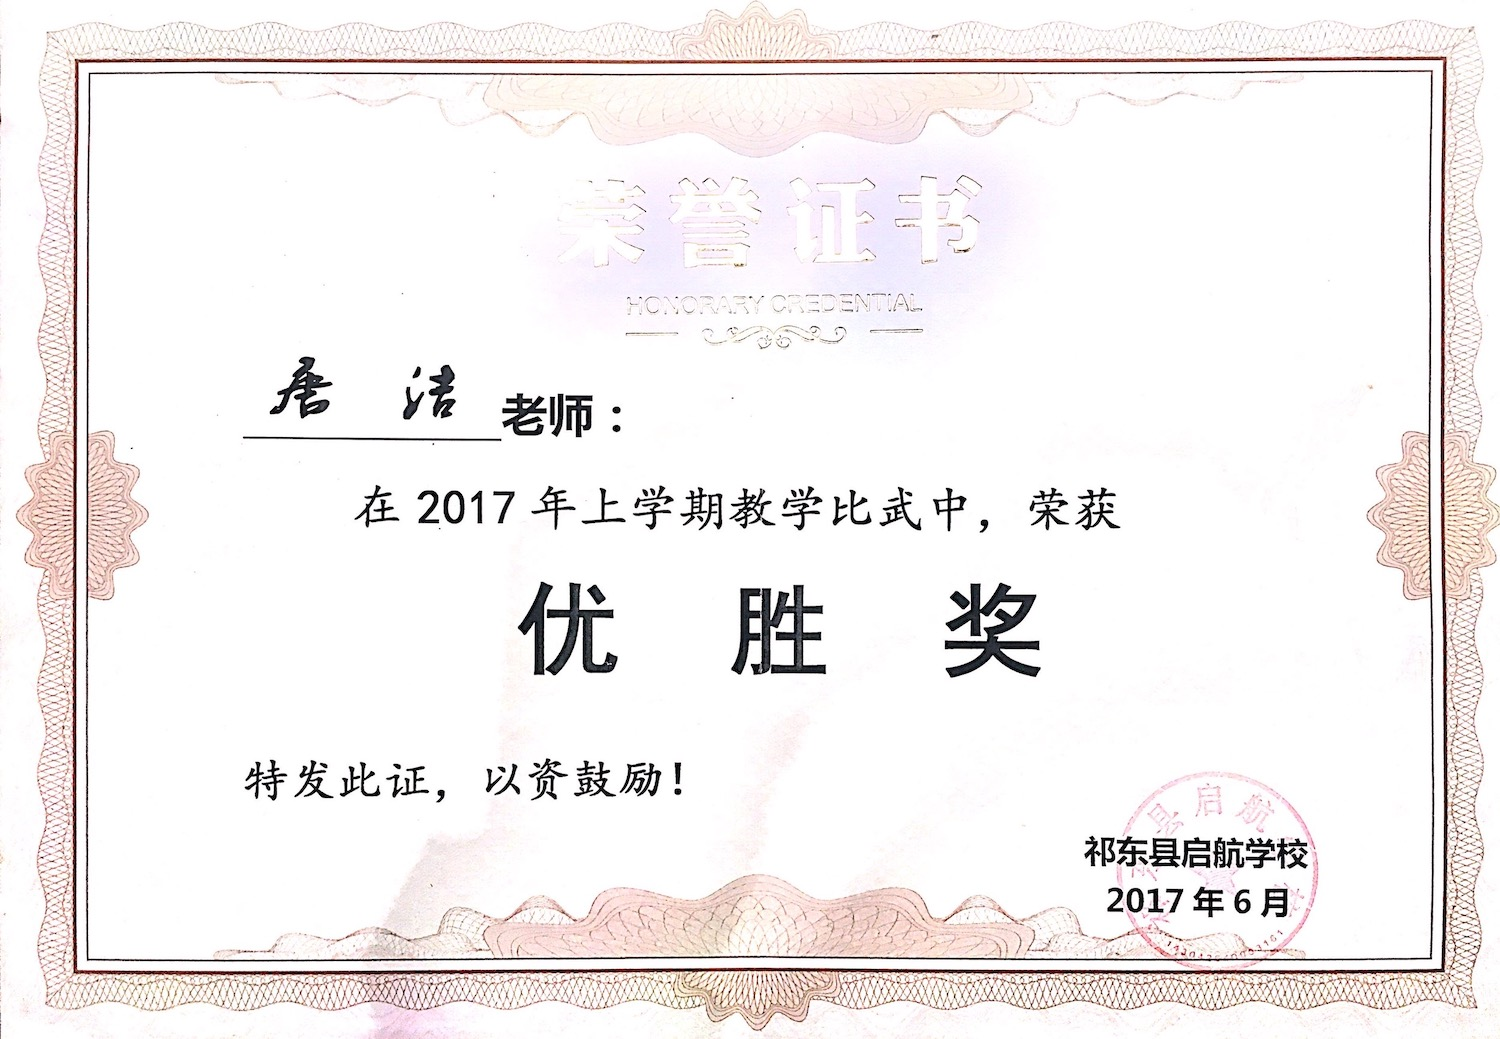
\includegraphics[scale=0.27]{figs/2017-06.jpg }
 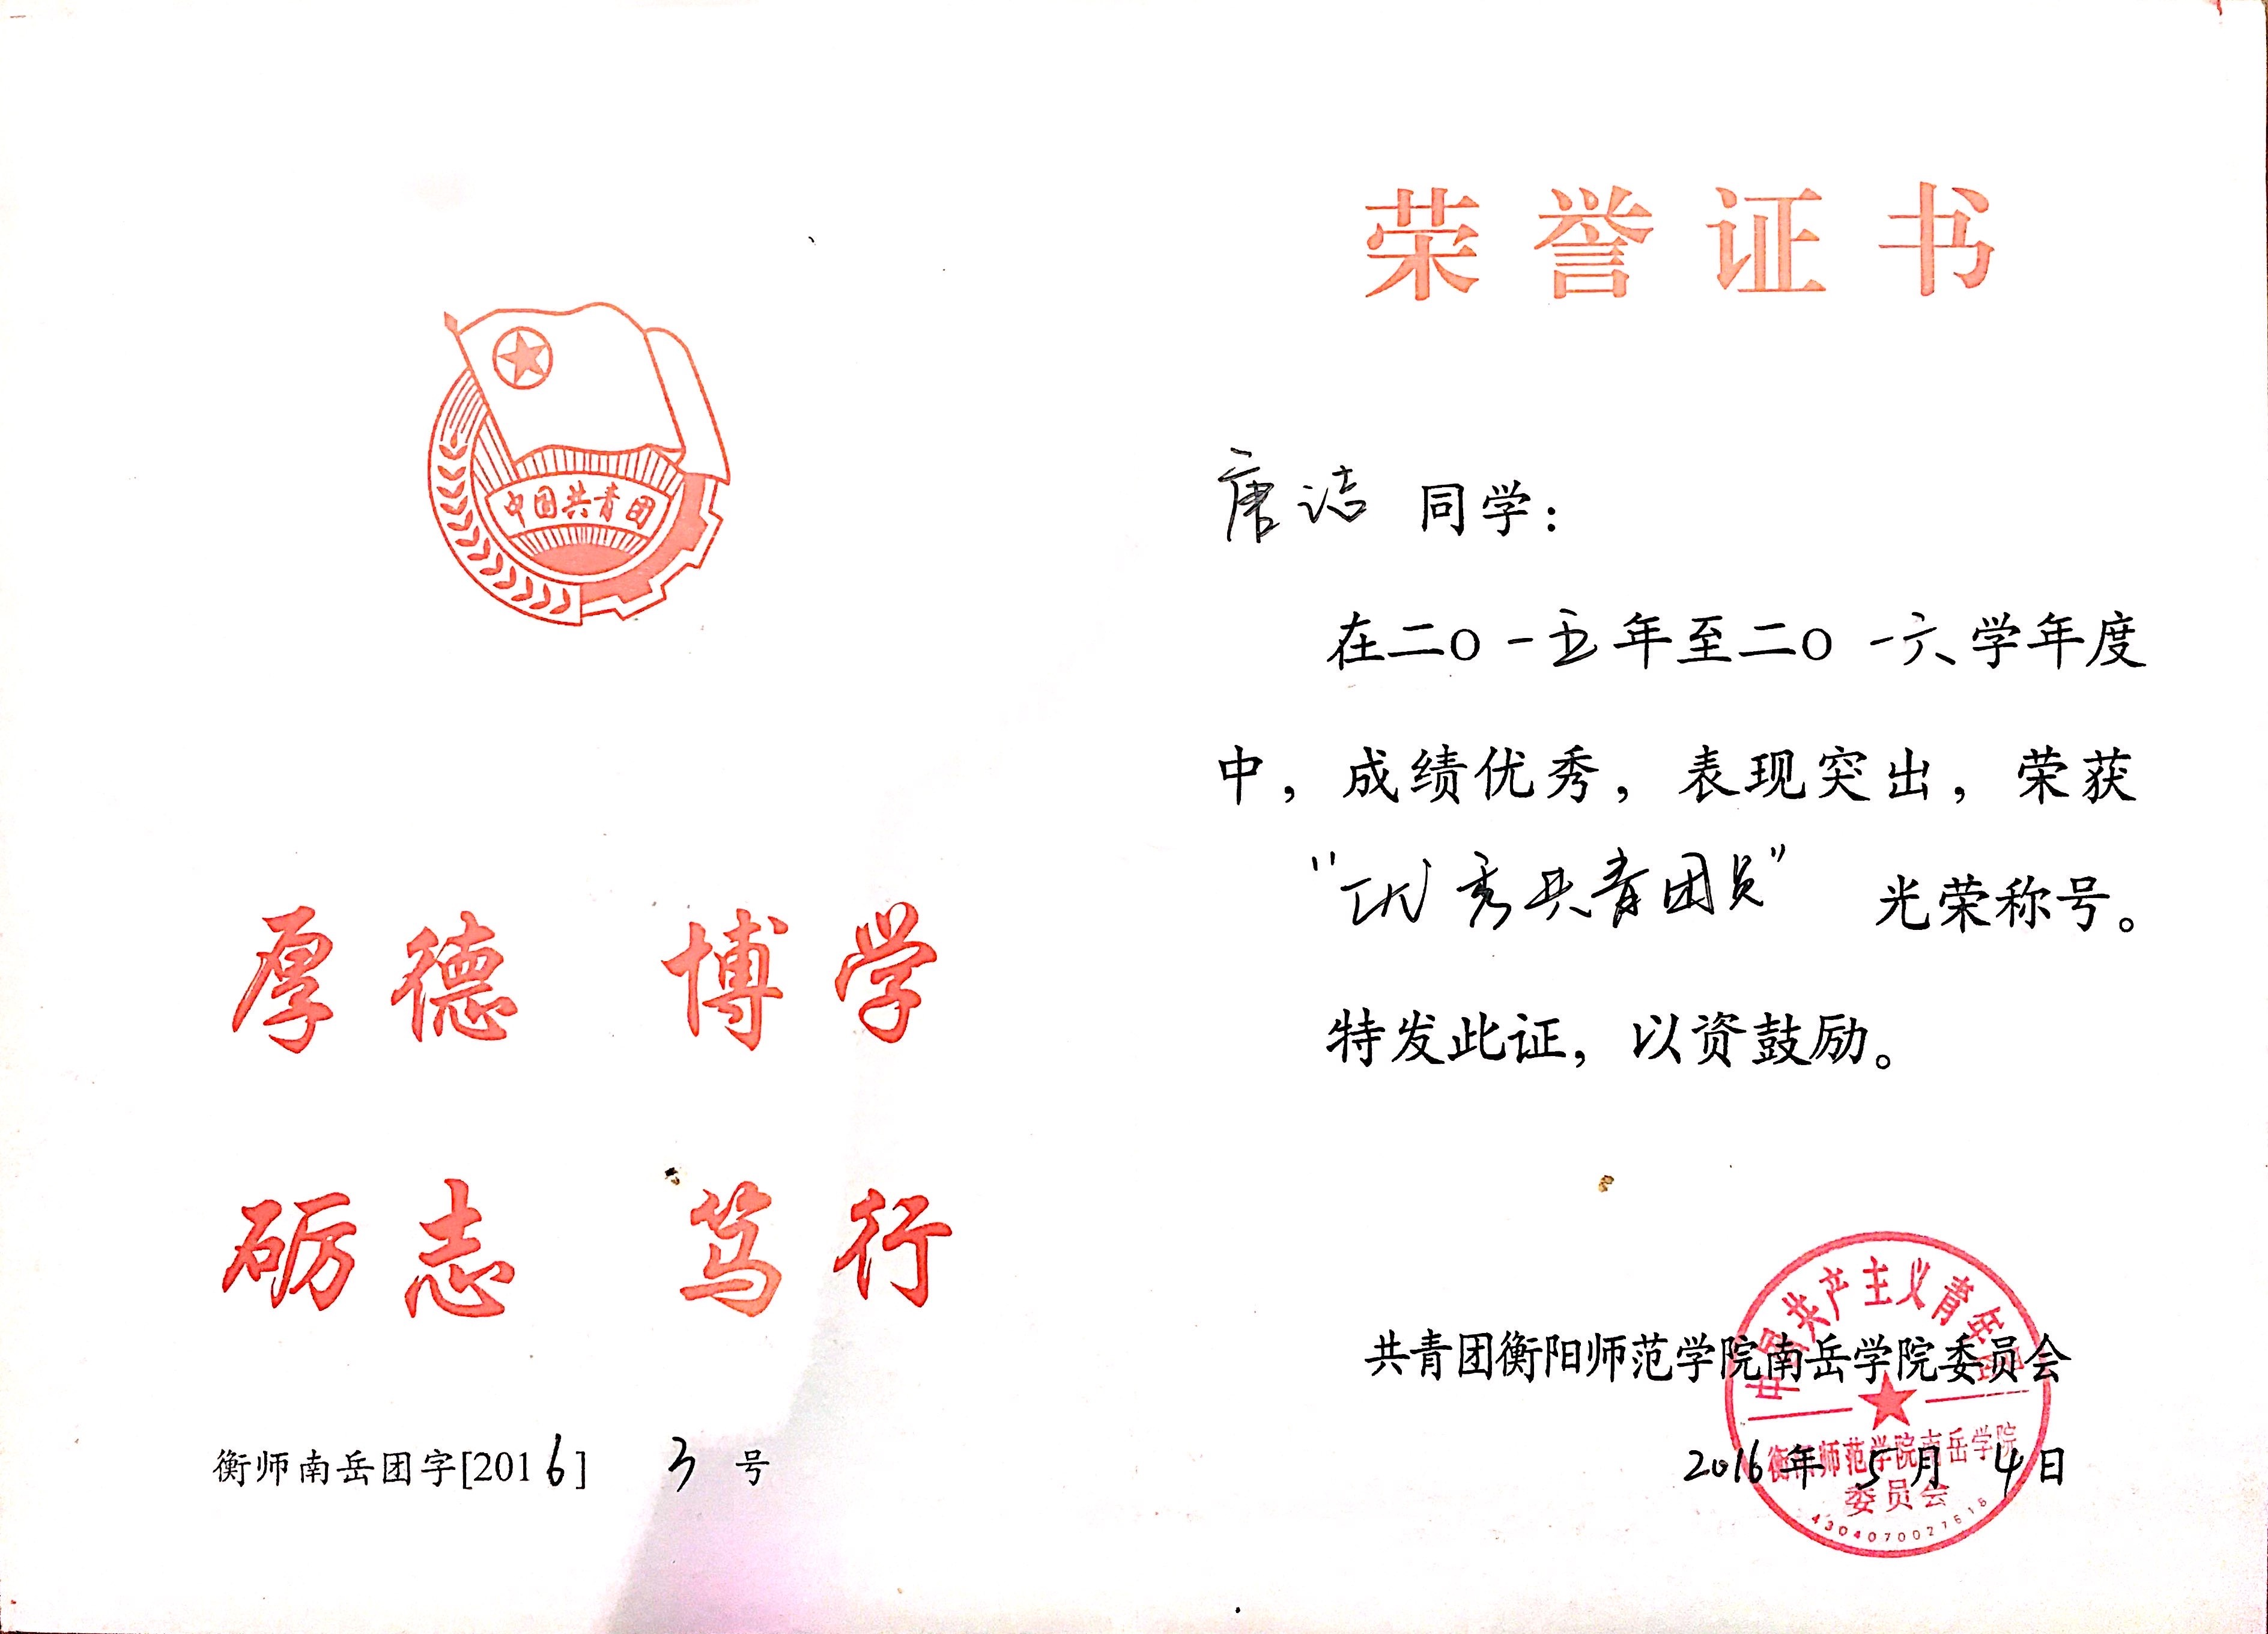
\includegraphics[scale=0.1]{figs/2016-05.jpg }
 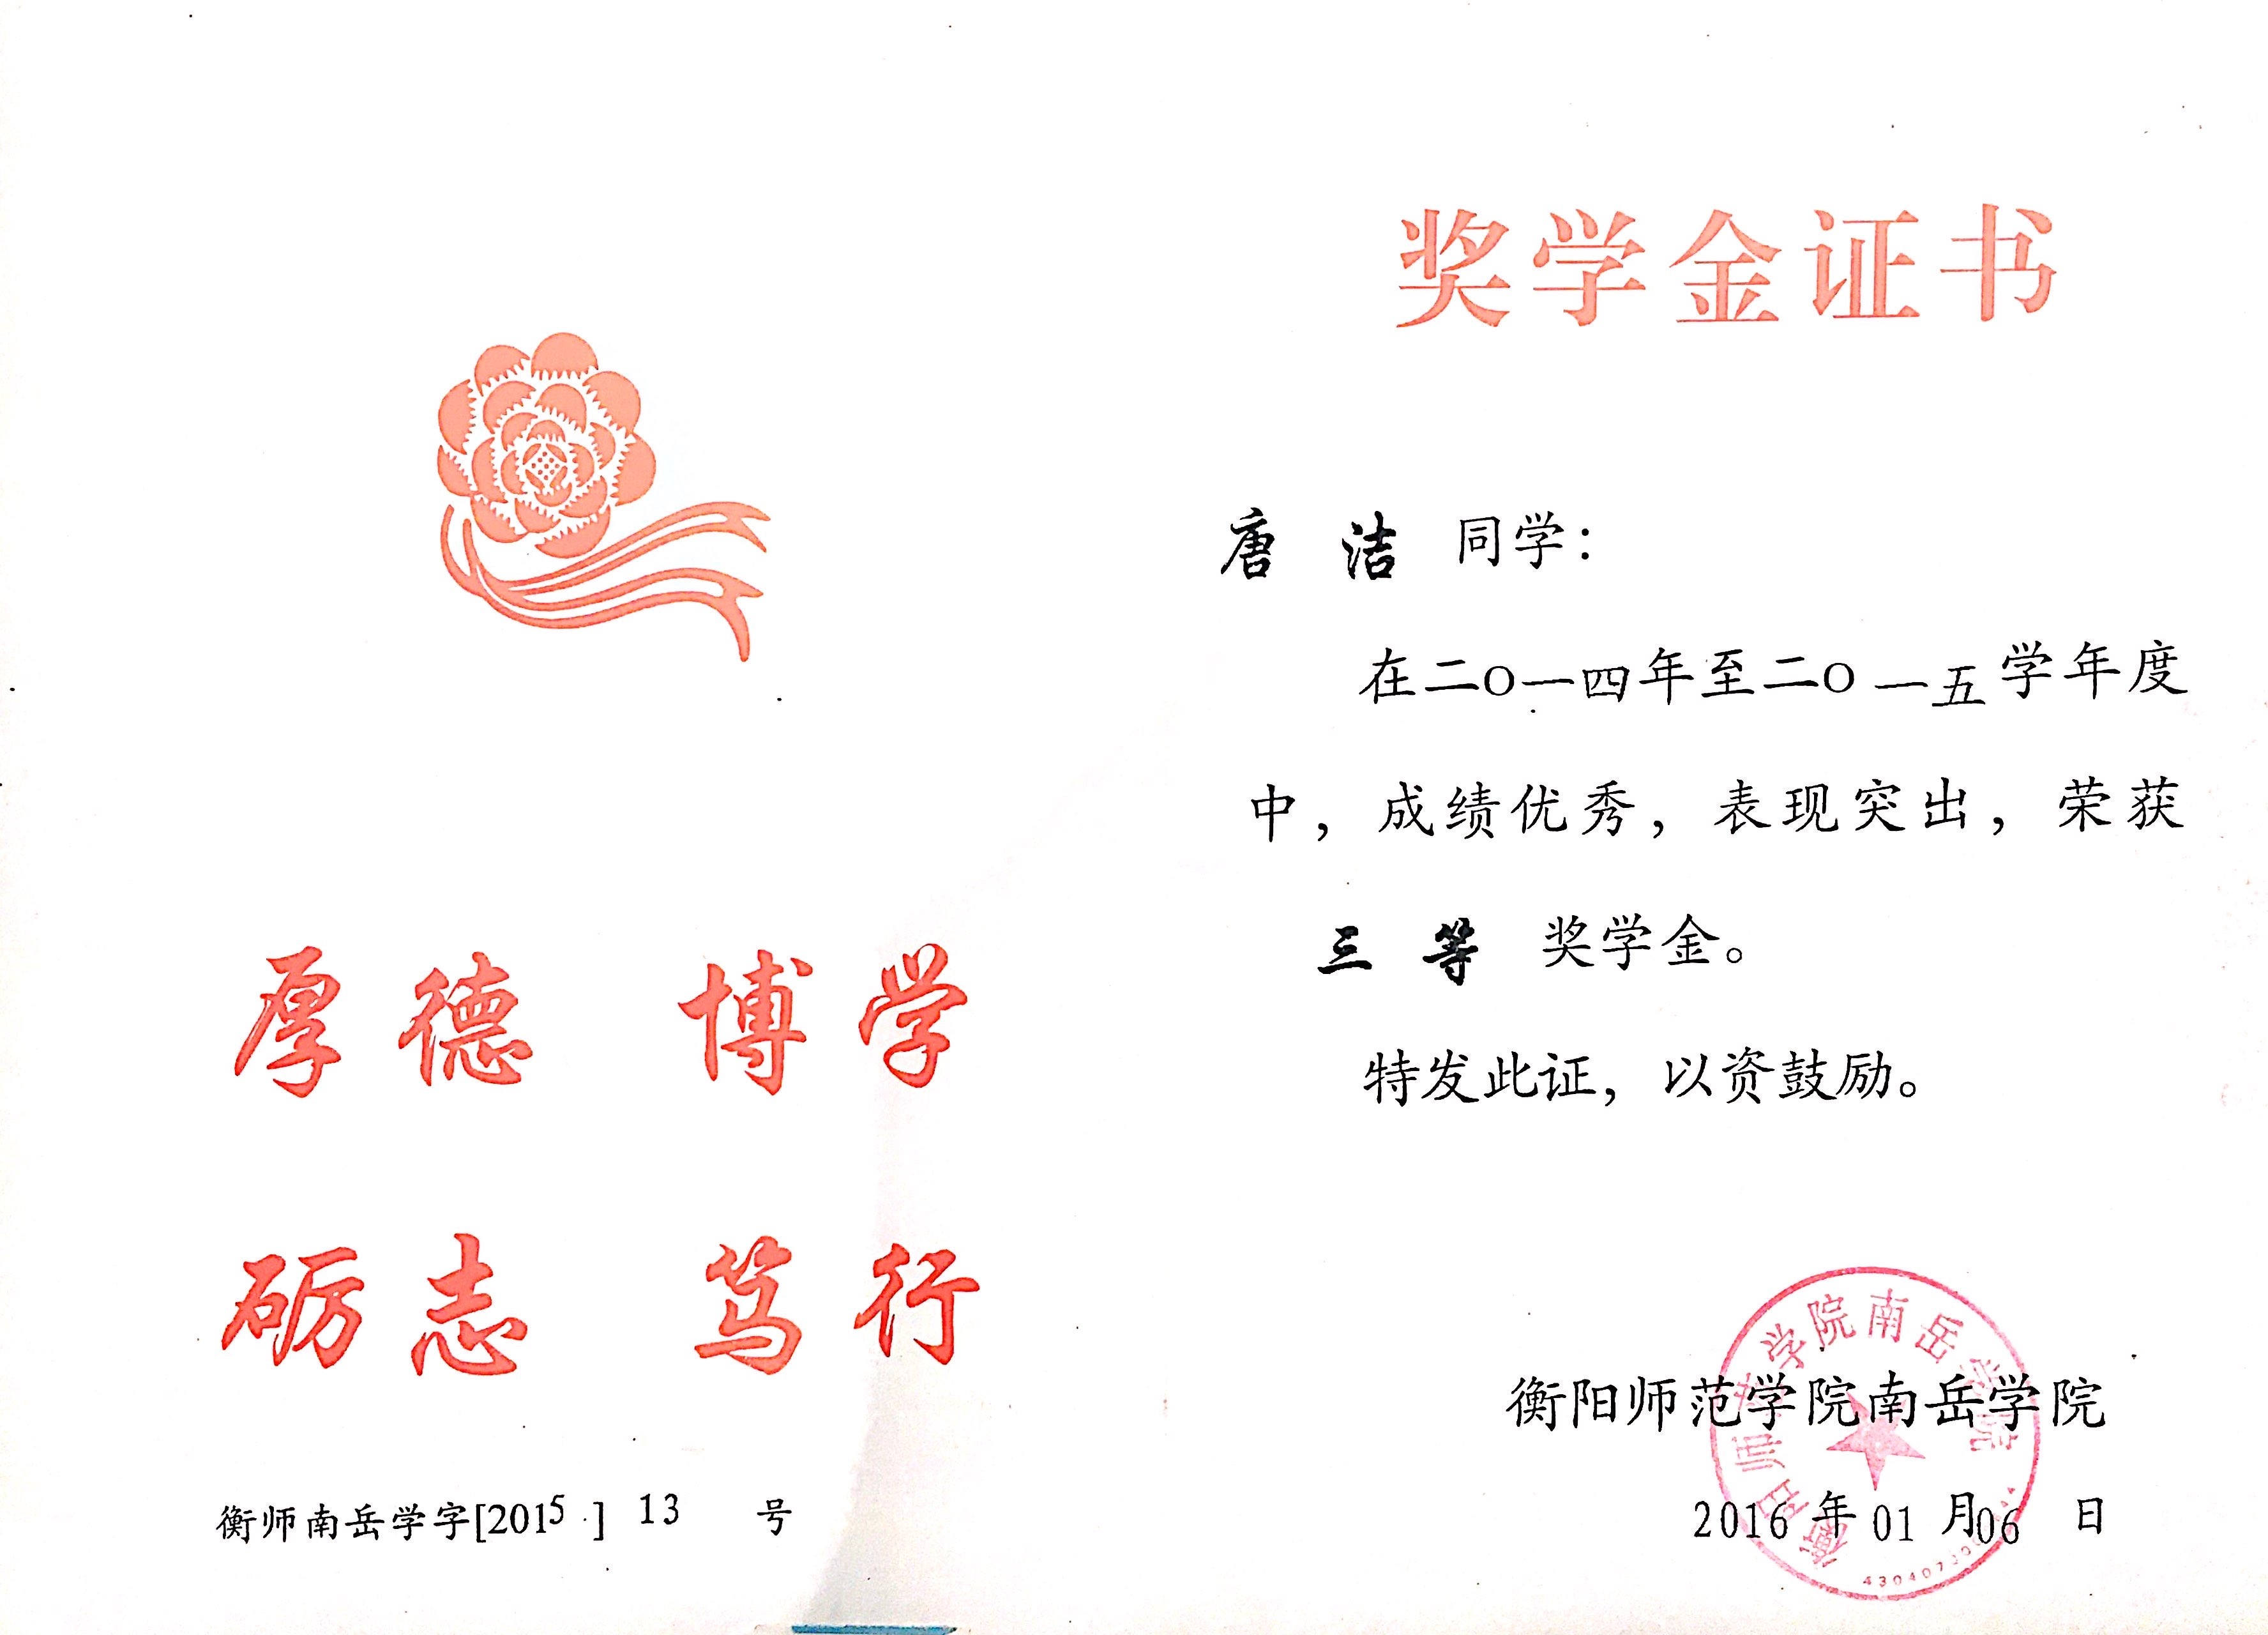
\includegraphics[scale=0.1]{figs/2016-01_1.jpg }
 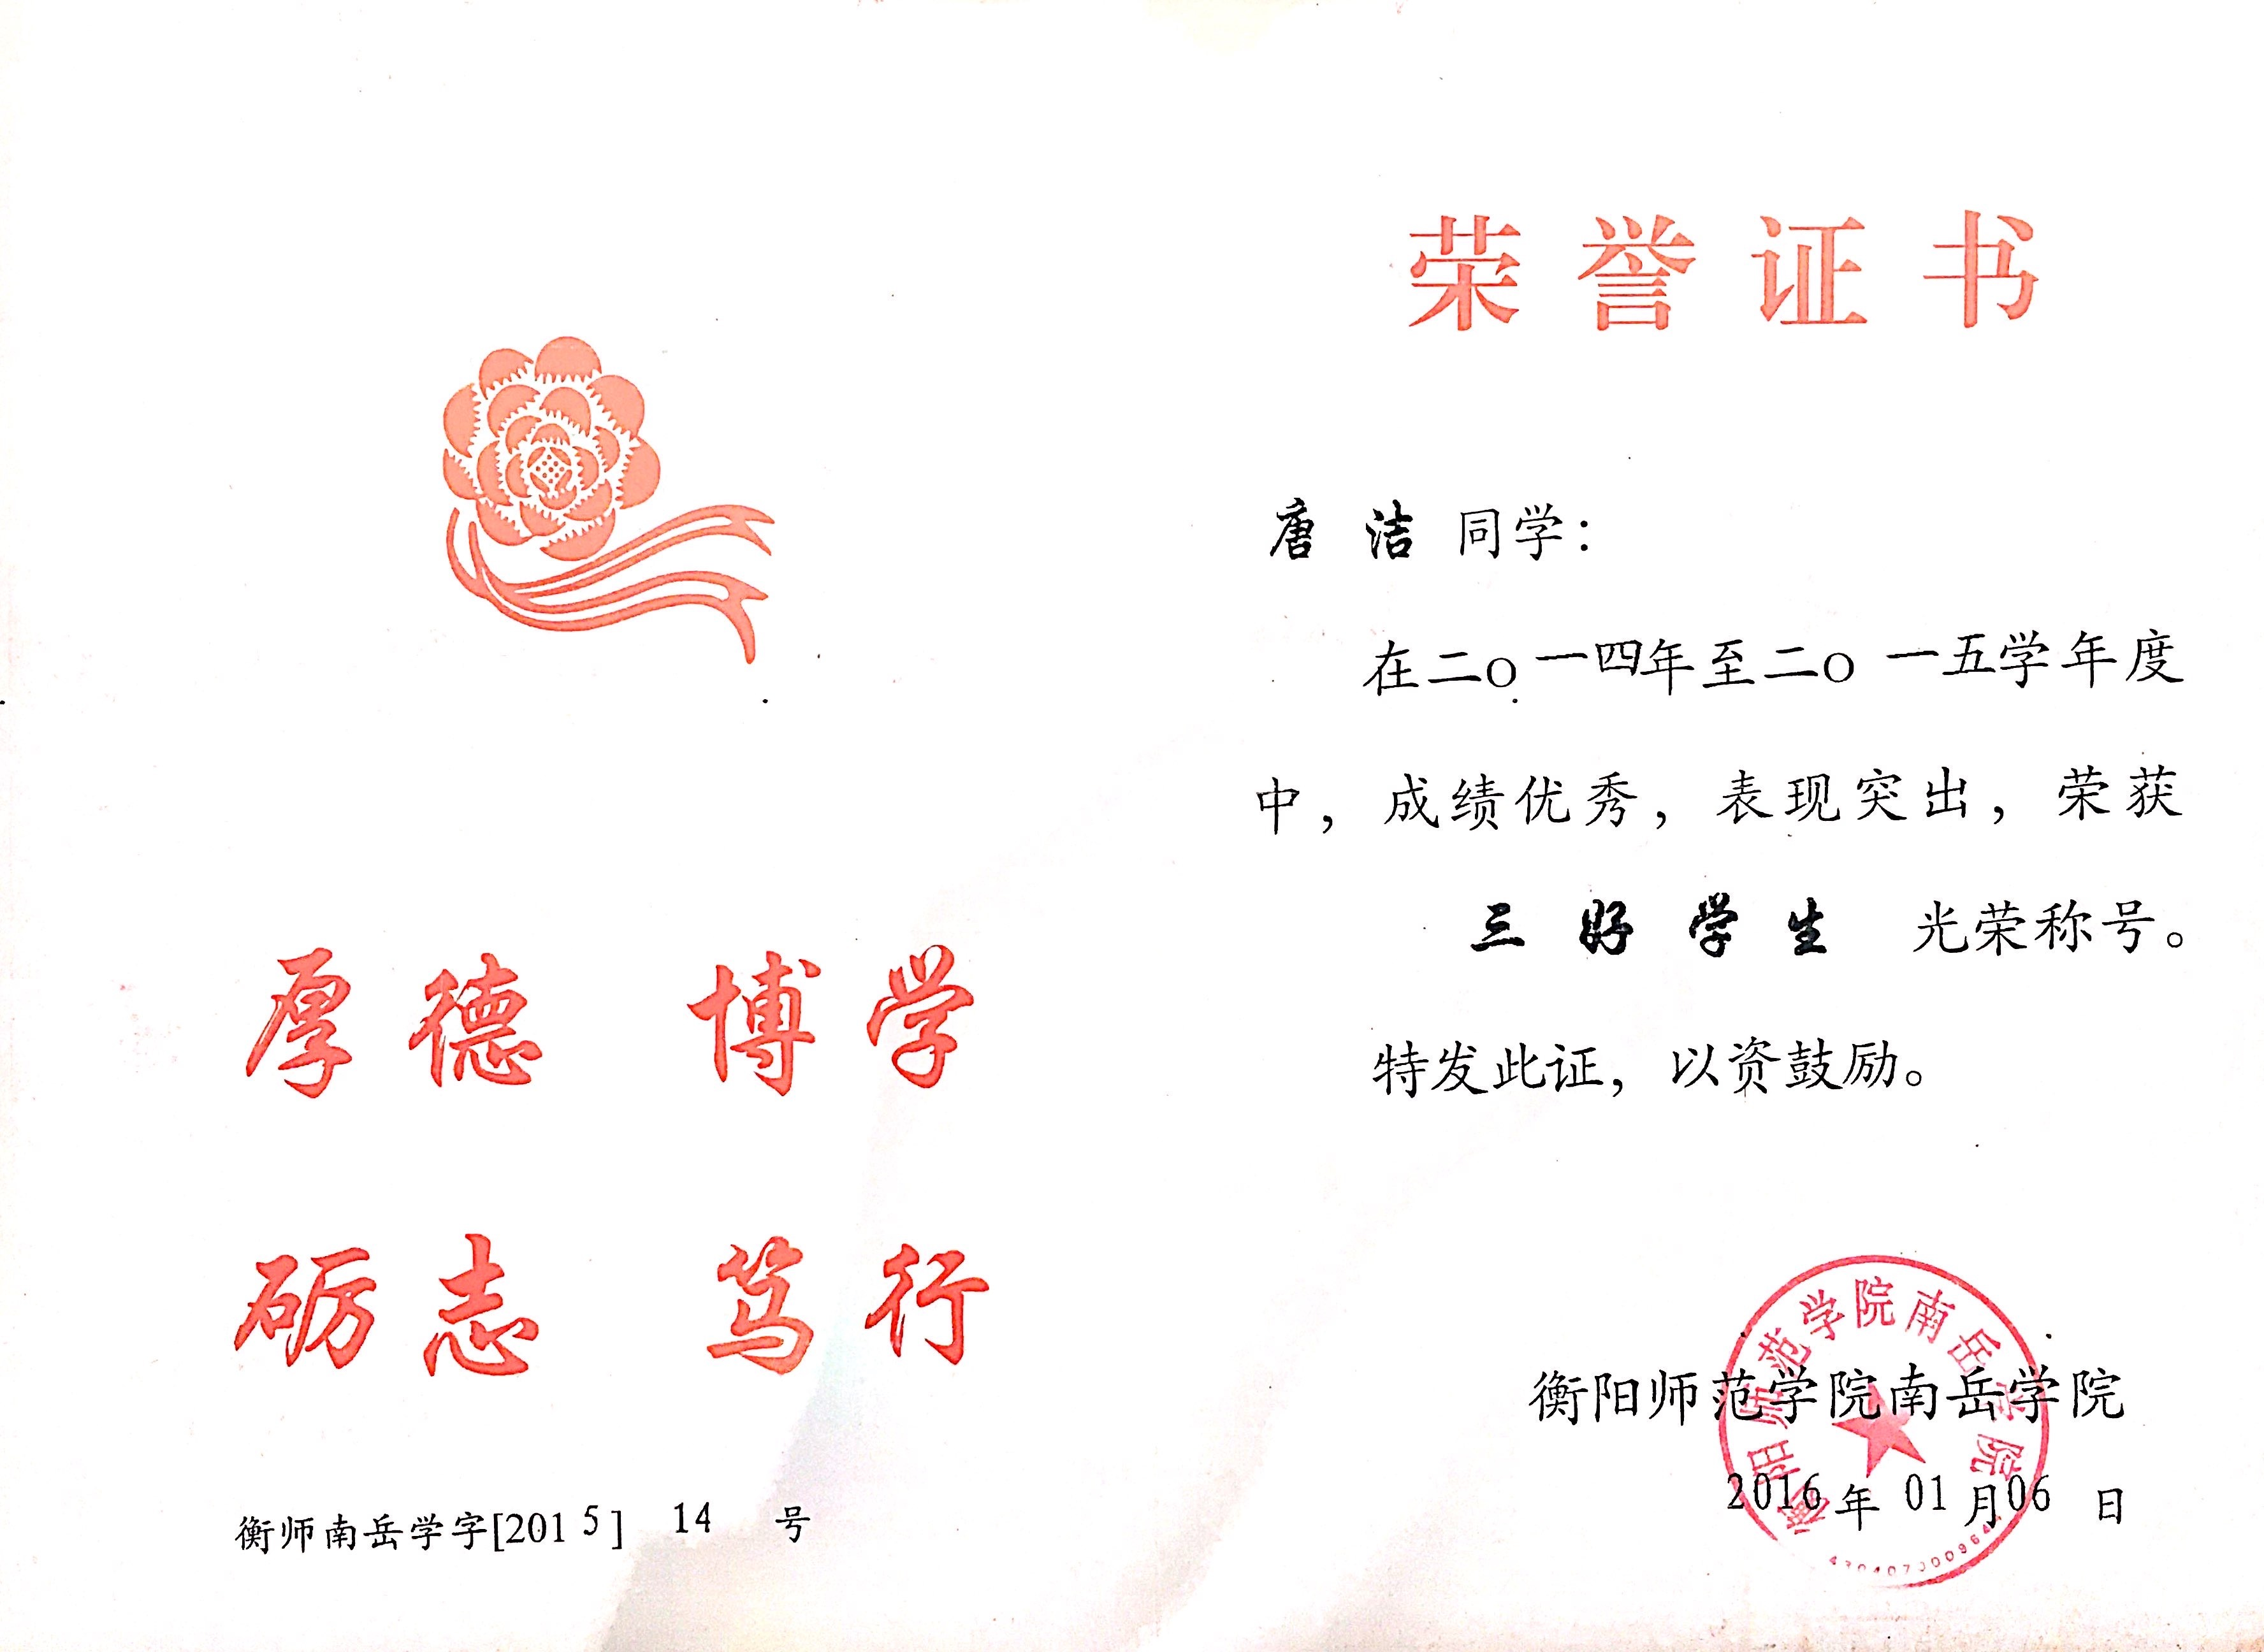
\includegraphics[scale=0.1]{figs/2016-01_2.jpg }
% 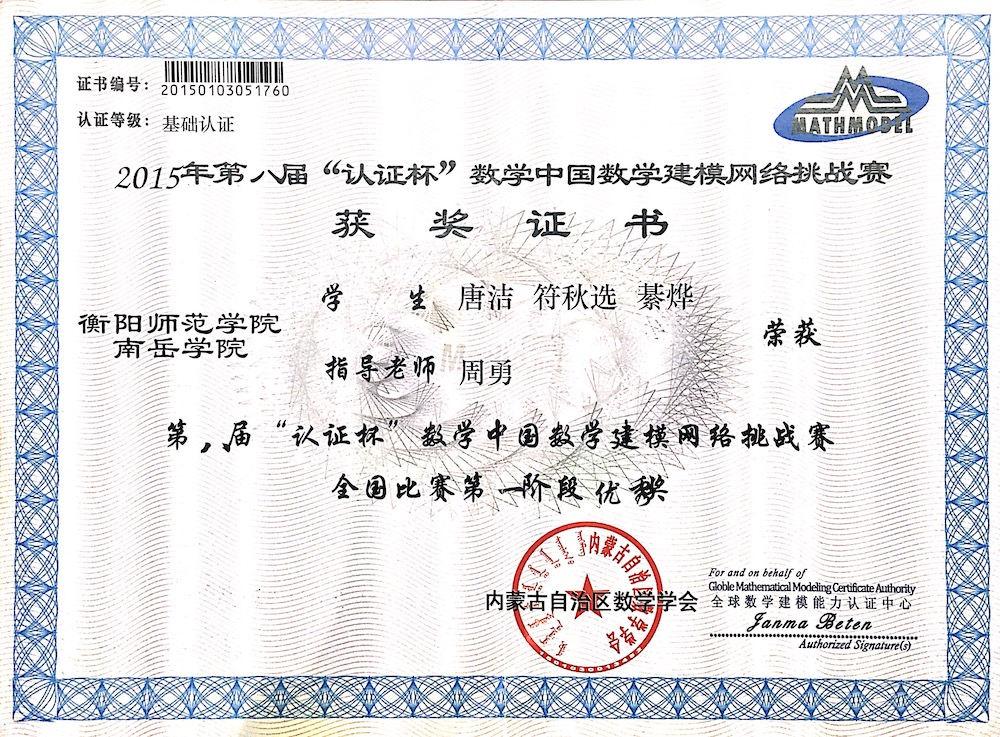
\includegraphics[scale=0.35]{figs/2015-09.jpg }
% 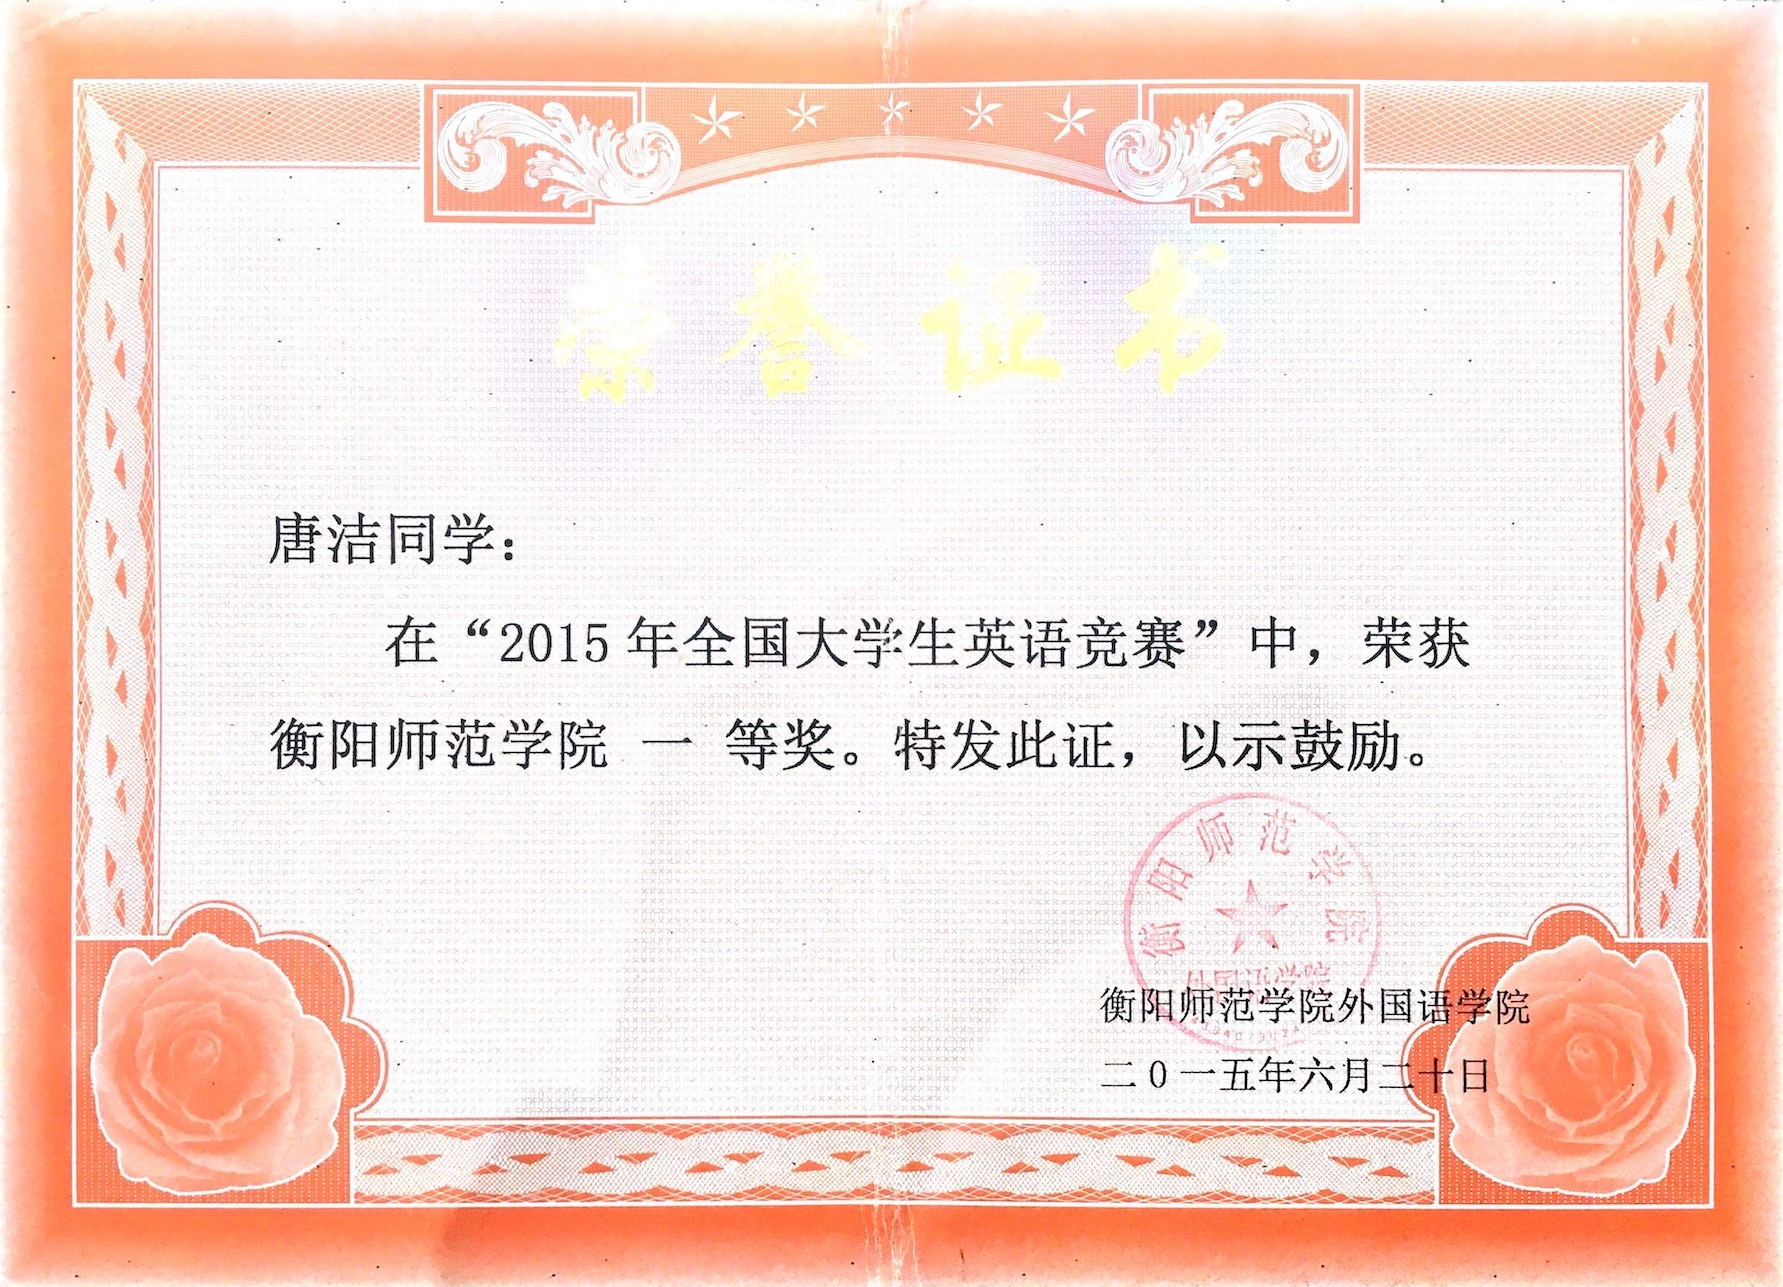
\includegraphics[scale=0.2]{figs/2015-06.jpg }
% 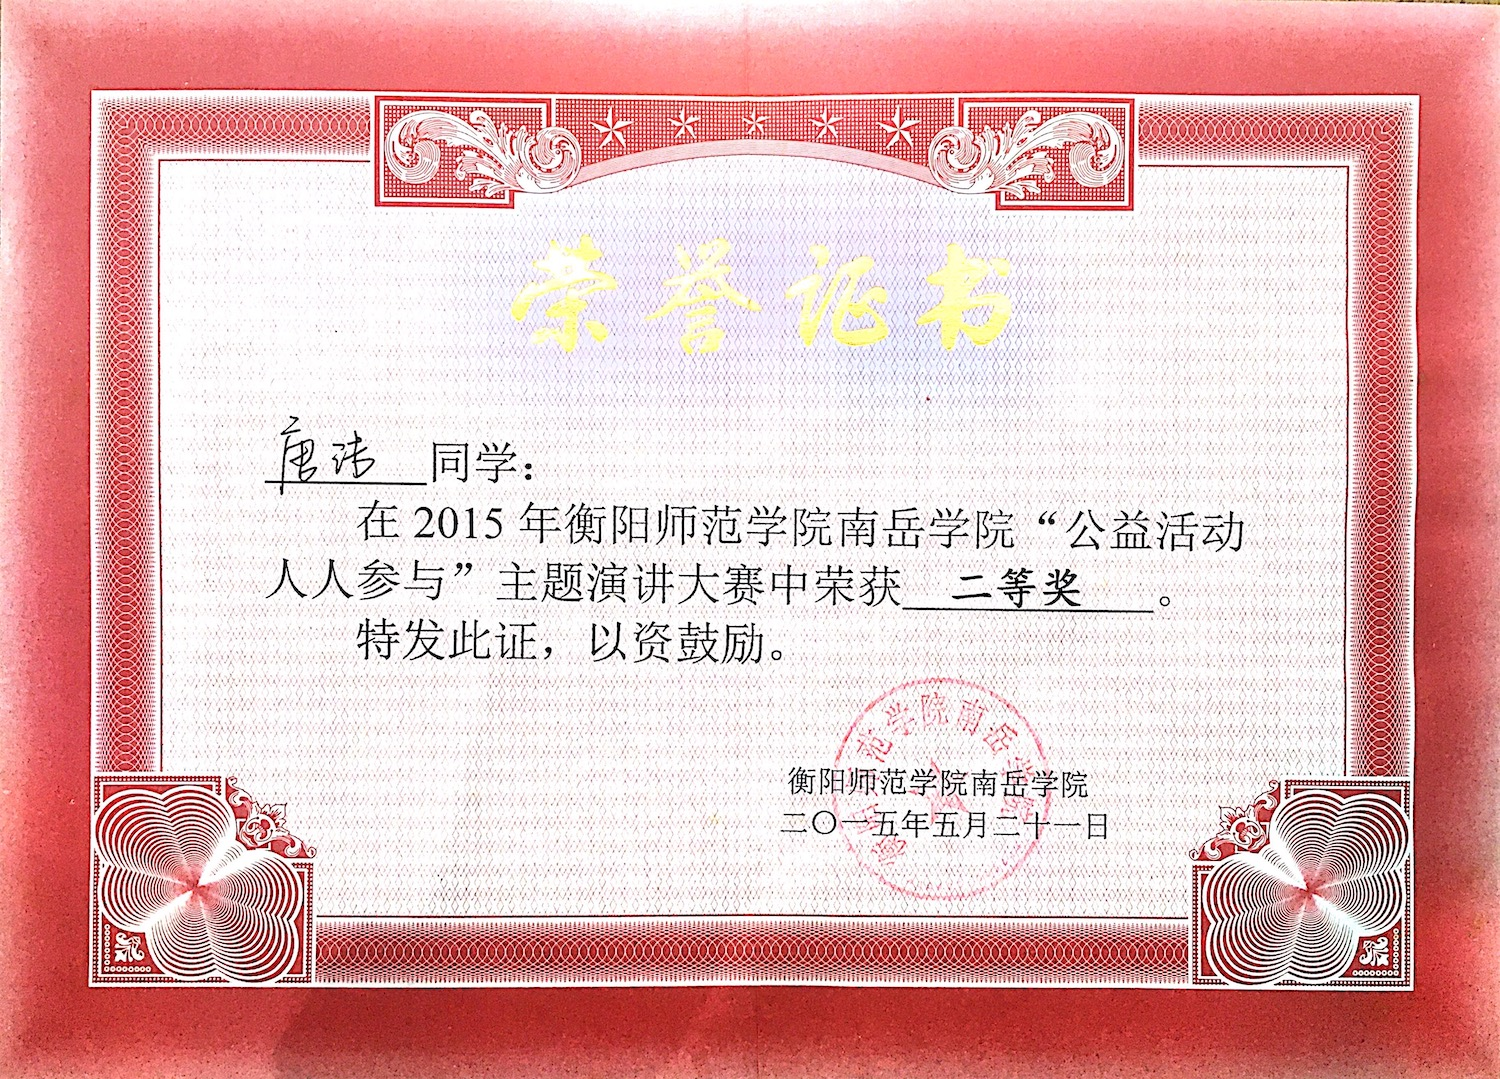
\includegraphics[scale=0.24]{figs/2015-05.jpg }
\end{center}


%\section{成绩单}
%\begin{center}
% 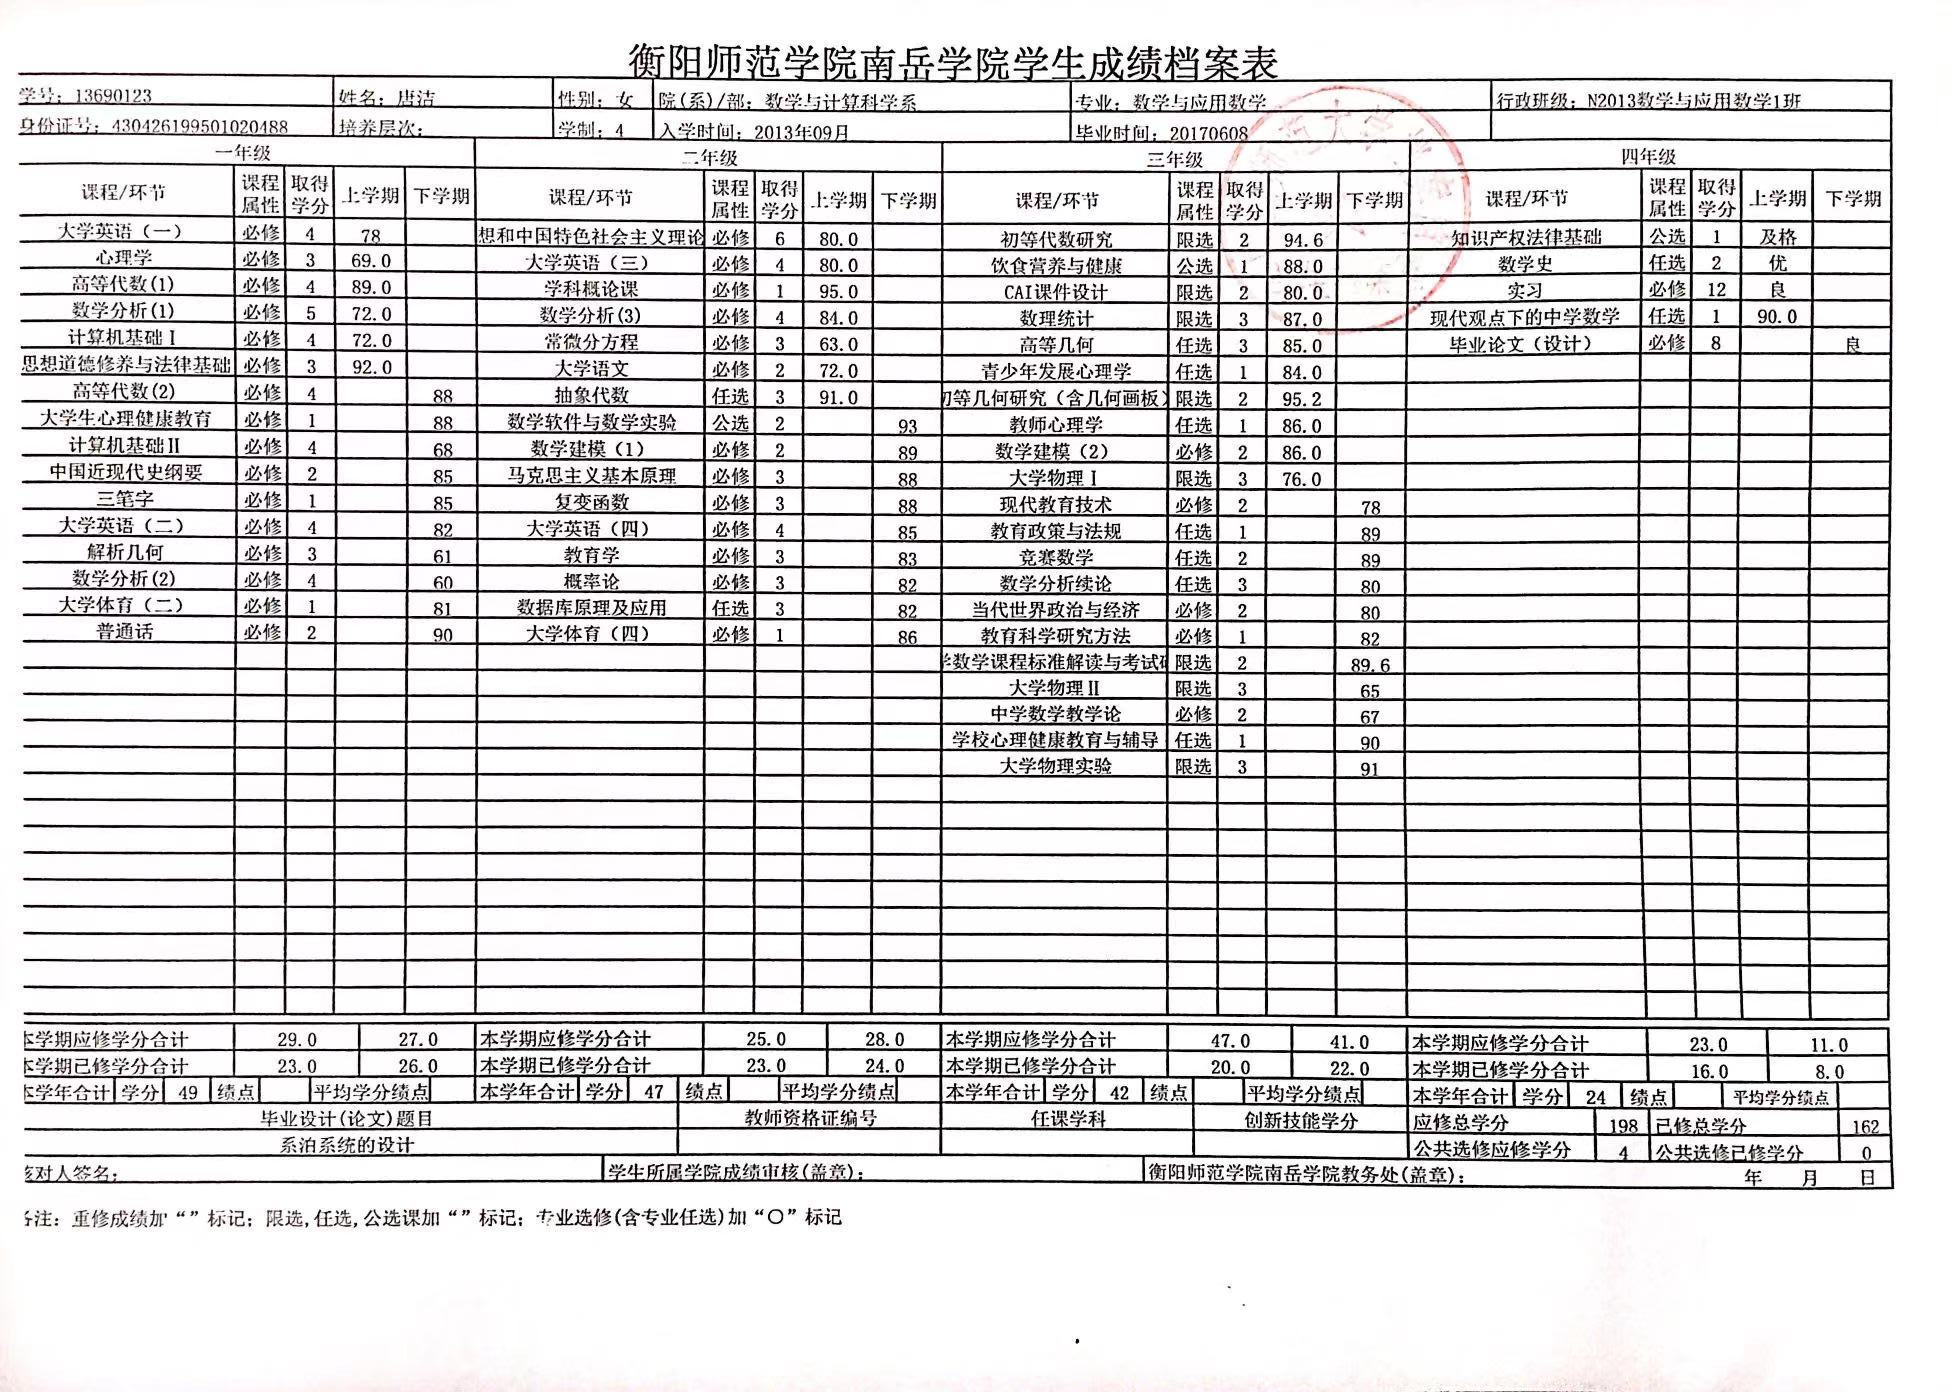
\includegraphics[scale=0.28]{figs/本科成绩单.jpg }
%  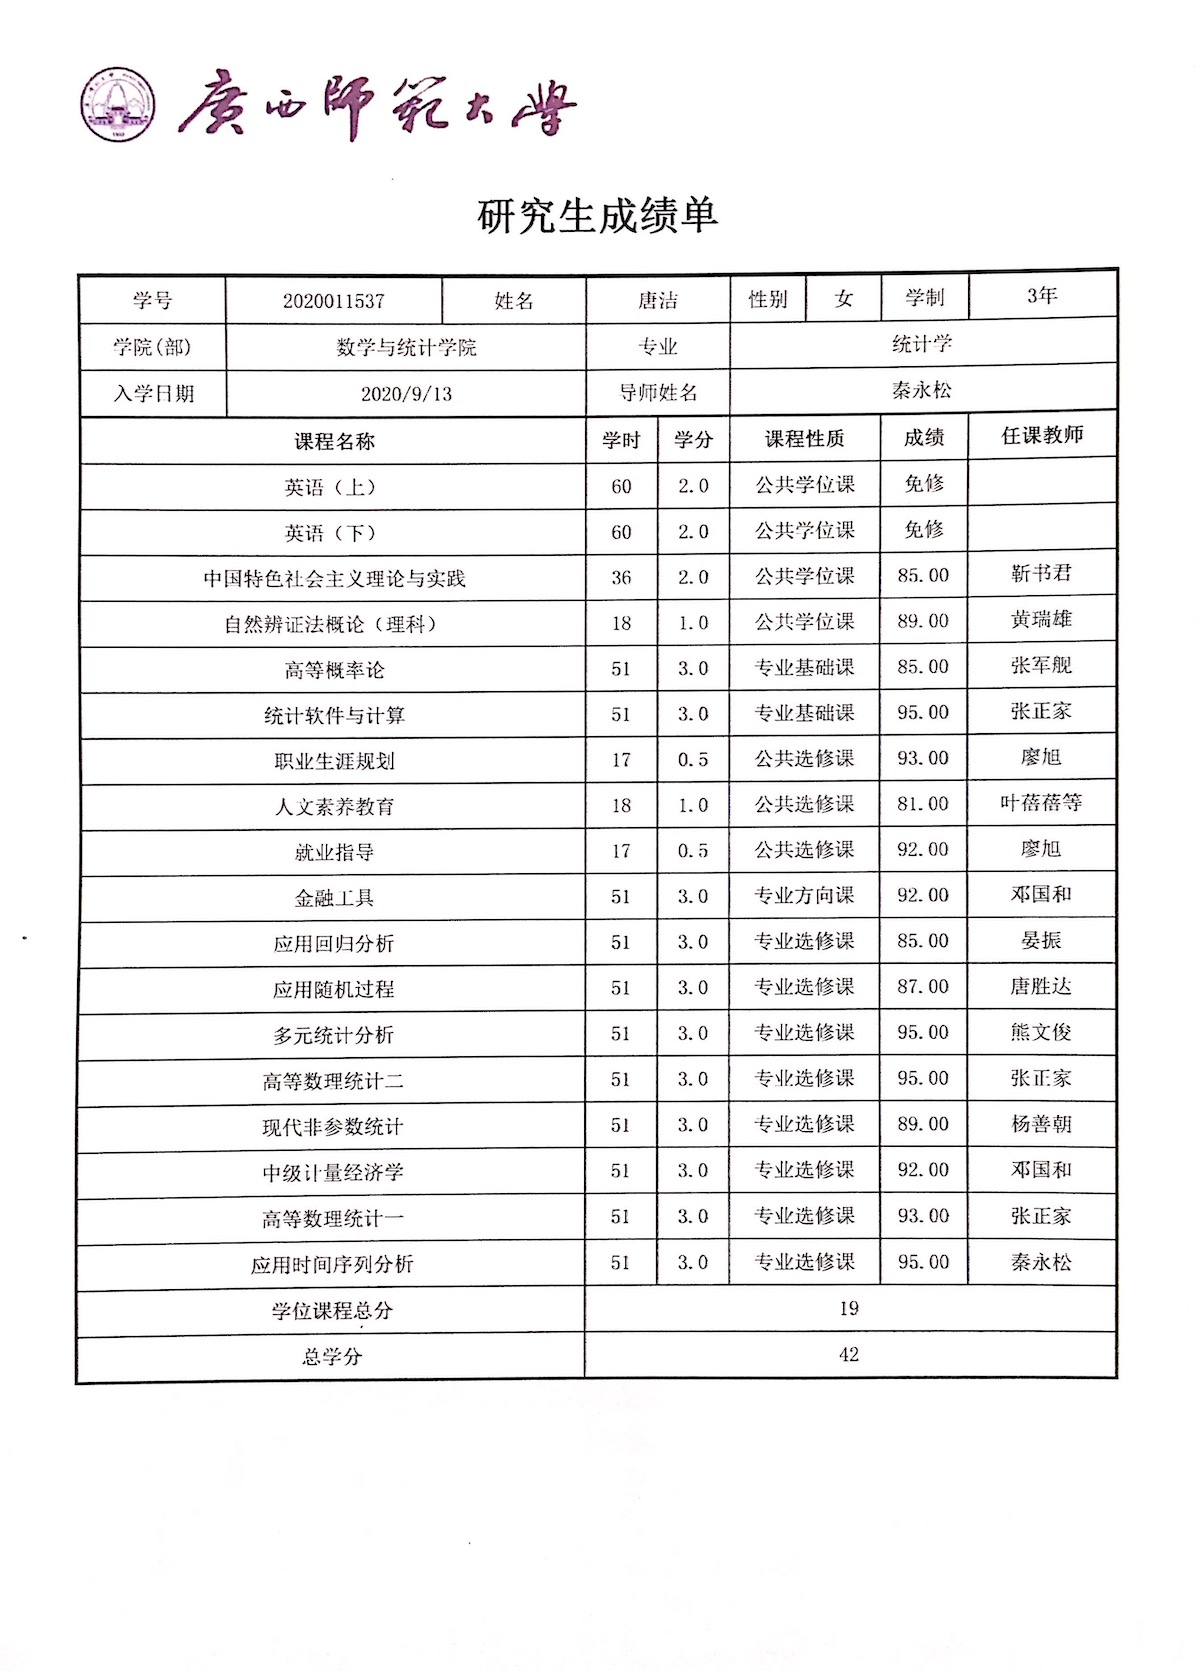
\includegraphics[scale=0.4]{figs/硕士成绩单1.jpg }
%  \includegraphics[scale=0.35]{figs/硕士成绩单2.jpg }
%\end{center}

%\section{攻读硕士学位期间取得成绩}
%
%\subsection{发表学术论文}
%
%\nh { \bfseries 唐洁}. 含空间自回归误差的空间自回归模型的经验欧氏似然推断[J]. 广西民族大学学报(自然科学版), 2021, 27(04): 70-74.
%
%\nh { \bfseries 唐洁}, 秦永松. 含空间自相关误差的空间自回归模型的调整经验似然推断. (投稿)
%
%\nh { \bfseries Tang Jie}, Qin Yongsong. Empirical likelihood for spatial dynamic panel data models with spatial errors and endogenous initial observations. (投稿)
%
%\nh { \bfseries Tang Jie}, Qin Yongsong. Adjusted empirical likelihood for probability density functions under strong mixing samples. (投稿)
%
%\nh { \bfseries Tang Jie}, Zou Yunlong, Qin Yongsong. Principal component empirical likelihood method for spatial data with a diverging number of parameters. (定稿)
%
%\nh Zou Yunlong, { \bfseries Tang Jie}, Qin Yongsong. Blockwise empirical likelihood method for spatial dependent data. (定稿)
%
%\nh Li Yufang, { \bfseries Tang Jie}, Qin Yongsong. Empirical likelihood ratio test for linear models with equality constraints. (投稿)
%
%\subsection{科研项目经历}
%
%2022年4月, 主持广西研究生教育创新计划项目 (YJSCXP202104) “空间计量经济模型的调整经验似然 ”, 唐洁 (1 / 5). 

\subsection{成绩单}
\includepdf[pages=1]{pdfs/成绩单硕士3.pdf}


%\includepdf[pages=1]{pdfs/硕士科研成果.pdf}

%\nh 唐洁.含空间自回归误差的空间自回归模型的经验欧氏似然推断[J].广西民族大学学报(自然科学版),2021,27(04):70-74.
%
%\nh  Tang Jie, Qin Yongsong. Adjusted empirical likelihood for probability density functions under strong mixing samples. (SCI四区期刊Communications in Statistics - Theory and Methods已接受录用)
%
%\includepdf[pages=1]{pdfs/含空间自回归误差的空间自回归模型的经验欧氏似然推断_唐洁.pdf}
%\includepdf[pages=1-2]{pdfs/Jay3.pdf}


\end{document}





